% ******************************* PhD Thesis Template **************************
% Please have a look at the README.md file for info on how to use the template

\documentclass[a4paper,custommargin,customfont,print,index,custombib]{Classes/PhDThesisPSnPDF}

% ******************************************************************************
% ******************************* Class Options ********************************
% *********************** See README for more details **************************
% ******************************************************************************

% `a4paper'(The University of Cambridge PhD thesis guidelines recommends a page
% size a4 - default option) or `a5paper': A5 Paper size is also allowed as per
% the Cambridge University Engineering Deparment guidelines for PhD thesis
%
% `11pt' or `12pt'(default): Font Size 10pt is NOT recommended by the University
% guidelines
%
% `oneside' or `twoside'(default): Printing double side (twoside) or single
% side.
%
% `print': Use `print' for print version with appropriate margins and page
% layout. Leaving the options field blank will activate Online version.
%
% `index': For index at the end of the thesis
%
% `draft': For draft mode without loading any images (same as draft in book)
%
% `draftmode': Special draft mode with line numbers, images, and water mark with
% timestamp and custom text. Position of the text can also be modified.
%
% `abstract': To generate only the title page and abstract page with
% dissertation title and name, to submit to the Student Registry
%
% `chapter`: This option enables only the specified chapter and it's references
%  Useful for review and corrections.
%
% ************************* Custom Page Margins ********************************
%
% `custommargin`: Use `custommargin' in options to activate custom page margins,
% which can be defined in the preamble.tex. Custom margin will override
% print/online margin setup.
%
% *********************** Choosing the Fonts in Class Options ******************
%
% `times' : Times font with math support. (The Cambridge University guidelines
% recommend using times)
%
% `fourier': Utopia Font with Fourier Math font (Font has to be installed)
%            It's a free font.
%
% `customfont': Use `customfont' option in the document class and load the
% package in the preamble.tex
%
% default or leave empty: `Latin Modern' font will be loaded.
%
% ********************** Choosing the Bibliography style ***********************
%
% `authoryear': For author-year citation eg., Krishna (2013)
%
% `numbered': (Default Option) For numbered and sorted citation e.g., [1,5,2]
%
% `custombib': Define your own bibliography style in the `preamble.tex' file.
%              `\RequirePackage[square, sort, numbers, authoryear]{natbib}'.
%              This can be also used to load biblatex instead of natbib
%              (See Preamble)
%
% **************************** Choosing the Page Style *************************
%
% `default (leave empty)': For Page Numbers in Header (Left Even, Right Odd) and
% Chapter Name in Header (Right Even) and Section Name (Left Odd). Blank Footer.
%
% `PageStyleI': Chapter Name next & Page Number on Even Side (Left Even).
% Section Name & Page Number in Header on Odd Side (Right Odd). Footer is empty.
%
% `PageStyleII': Chapter Name on Even Side (Left Even) in Header. Section Number
% and Section Name in Header on Odd Side (Right Odd). Page numbering in footer


% ********************************** Preamble **********************************
% Preamble: Contains packages and user-defined commands and settings
% ******************************************************************************
% ****************************** Custom Margin *********************************

% Add `custommargin' in the document class options to use this section
% Set {innerside margin / outerside margin / topmargin / bottom margin}  and
% other page dimensions
\ifsetCustomMargin
  \RequirePackage[left=34mm,right=50mm,top=32mm,bottom=60mm]{geometry}
  \setFancyHdr % To apply fancy header after geometry package is loaded
  \setlength{\headheight}{26pt} 
\fi

% *****************************************************************************
% ******************* Fonts (like different typewriter fonts etc.)*************

% Add `customfont' in the document class option to use this section

\ifsetCustomFont
  % Set your custom font here and use `customfont' in options. Leave empty to
  % load computer modern font (default LaTeX font).
  % \RequirePackage{helvet}
  \RequirePackage{tgpagella}
  \RequirePackage{gillius2}
  
\fi

\newcommand*\name[1]{\textsf{#1}}

% *****************************************************************************
% **************************** Custom Packages ********************************

% ************************* Algorithms and Pseudocode **************************

%\usepackage{algpseudocode}


% ********************Captions and Hyperreferencing / URL **********************

% Captions: This makes captions of figures use a boldfaced small font.
%\RequirePackage[small,bf]{caption}

\usepackage{hyperref}

\RequirePackage[labelsep=space,tableposition=top]{caption}
\renewcommand{\figurename}{Fig.} %to support older versions of captions.sty
\renewcommand{\captionfont}{\sffamily\small}

\RequirePackage[footfont=Large,style=ruled,footposition=caption]{floatrow}

\newcommand{\textunderscript}[1]{$_{\text{#1}}$}

% \newcommand*\legend[1]{\small{\textsf{#1}}}


% *************************** Graphics and figures *****************************

%\usepackage{rotating}
\usepackage{wrapfig}

% Uncomment the following two lines to force Latex to place the figure.
% Use [H] when including graphics. Note 'H' instead of 'h'
\usepackage{float}
\restylefloat{figure}

% Subcaption package is also available in the sty folder you can use that by
% uncommenting the following line
% This is for people stuck with older versions of texlive
% \usepackage{sty/caption/subcaption}
% \usepackage{subcaption}


% ********************************** Tables ************************************
\usepackage{booktabs} % For professional looking tables
\usepackage{multirow}

%\usepackage{multicol}
%\usepackage{longtable}
\usepackage{tabularx}


% ***************************** Math and SI Units ******************************

\usepackage{amsfonts}
\usepackage{amsmath}
\usepackage{amssymb}
\usepackage{siunitx} % use this package module for SI units
\usepackage{bm}

\usepackage{xfrac}


% ******************************* Line Spacing *********************************

% Choose linespacing as appropriate. Default is one-half line spacing as per the
% University guidelines

% \doublespacing
% \onehalfspacing
% \singlespacing


% ************************ Formatting / Footnote *******************************

% Don't break enumeration (etc.) across pages in an ugly manner (default 10000)
%\clubpenalty=500
%\widowpenalty=500

%\usepackage[perpage]{footmisc} %Range of footnote options


% *****************************************************************************
% *************************** Bibliography  and References ********************

%\usepackage{cleveref} %Referencing without need to explicitly state fig /table

% Add `custombib' in the document class option to use this section
\ifuseCustomBib
   \RequirePackage[round, sort, authoryear]{natbib} % CustomBib
   \renewcommand\cite{\citep}

% If you would like to use biblatex for your reference management, as opposed to the default `natbibpackage` pass the option `custombib` in the document class. Comment out the previous line to make sure you don't load the natbib package. Uncomment the following lines and specify the location of references.bib file

%\RequirePackage[backend=biber, style=numeric-comp, citestyle=numeric, sorting=nty, natbib=true]{biblatex}
%\bibliography{References/references} %Location of references.bib only for biblatex

\fi

% changes the default name `Bibliography` -> `References'
\renewcommand{\bibname}{References}


% *****************************************************************************
% *************** Changing the Visual Style of Chapter Headings ***************
% This section on visual style is from https://github.com/cambridge/thesis

% Uncomment the section below. Requires titlesec package.

\RequirePackage{titlesec}

\titleformat{\section}[hang]{\normalfont\rmfamily\tiny}{\thesection}{1em}{\sffamily\large}{}

\titleformat{\subsection}[runin]{\normalfont\rmfamily\tiny}{\thesubsection}{1em}{\bfseries\sffamily\lsstyle\small}{}

\newcommand{\PreContentTitleFormat}{\titleformat{\chapter}[display]{\scshape\Large}
{\Large\filleft{\chaptertitlename} \Huge\thechapter}
{1ex}{}
[\vspace{1ex}\titlerule]}

\newcommand{\ContentTitleFormat}{\titleformat{\chapter}[display]{\scshape\huge}
{\Large\filleft{\chaptertitlename} \Huge\thechapter}{1ex}
{\titlerule\vspace{1ex}\filright}
[\vspace{1ex}\titlerule]}

\newcommand{\PostContentTitleFormat}{\PreContentTitleFormat}

\PreContentTitleFormat



% ******************************************************************************
% ************************* User Defined Commands ******************************
% ******************************************************************************

% *********** To change the name of Table of Contents / LOF and LOT ************

%\renewcommand{\contentsname}{My Table of Contents}
%\renewcommand{\listfigurename}{My List of Figures}
%\renewcommand{\listtablename}{My List of Tables}


% ********************** TOC depth and numbering depth *************************

\setcounter{secnumdepth}{2}
\setcounter{tocdepth}{2}


% ******************************* Nomenclature *********************************

% To change the name of the Nomenclature section, uncomment the following line

%\renewcommand{\nomname}{Symbols}


% ********************************* Appendix ***********************************

% The default value of both \appendixtocname and \appendixpagename is `Appendices'. These names can all be changed via:

%\renewcommand{\appendixtocname}{List of appendices}
%\renewcommand{\appendixname}{Appndx}

% ******************************** Draft Mode **********************************

% Uncomment to disable figures in `draftmode'
%\setkeys{Gin}{draft=true}  % set draft to false to enable figures in `draft'

% These options are active only during the draft mode
% Default text is "Draft"
%\SetDraftText{DRAFT}

% Default Watermark location is top. Location (top/bottom)
%\SetDraftWMPosition{bottom}

% Draft Version - default is v1.0
%\SetDraftVersion{v1.1}

% Draft Text grayscale value (should be between 0-black and 1-white)
% Default value is 0.75
%\SetDraftGrayScale{0.8}


%% Todo notes functionality
%% Uncomment the following lines to have todonotes.

%\ifsetDraft
%	\usepackage[colorinlistoftodos]{todonotes}
%	\newcommand{\mynote}[1]{\todo[author=kks32,size=\small,inline,color=green!40]{#1}}
%\else
%	\newcommand{\mynote}[1]{}
%	\newcommand{\listoftodos}{}
%\fi

% Example todo: \mynote{Hey! I have a note}



%% Short-hand for bold font commands

\newcommand{\unit}{{\bf I}}
\newcommand{\boldzero}{{\bf 0}}

\newcommand{\bfa}{{\bf a}}
\newcommand{\bfb}{{\bf b}}
\newcommand{\bfc}{{\bf c}}
\newcommand{\bfd}{{\bf d}}
\newcommand{\bfe}{{\bf e}}
\newcommand{\bff}{{\bf f}}
\newcommand{\bfg}{{\bf g}}
\newcommand{\bfh}{{\bf h}}
\newcommand{\bfi}{{\bf i}}
\newcommand{\bfk}{{\bf k}}
\newcommand{\bfl}{{\bf l}}
\newcommand{\bfm}{{\bf m}}
\newcommand{\bfp}{{\bf p}}
\newcommand{\bfr}{{\bf r}}
\newcommand{\bfs}{{\bf s}}
\newcommand{\bft}{{\bf t}}
\newcommand{\bfu}{{\bf u}}
\newcommand{\bfv}{{\bf v}}
\newcommand{\bfw}{{\bf w}}
\newcommand{\bfx}{{\bf x}}
\newcommand{\bfy}{{\bf y}}
\newcommand{\bfz}{{\bf z}}

\newcommand{\bfA}{{\bf A}}
\newcommand{\bfB}{{\bf B}}
\newcommand{\bfC}{{\bf C}}
\newcommand{\bfD}{{\bf D}}
\newcommand{\bfG}{{\bf G}}
\newcommand{\bfH}{{\bf H}}
\newcommand{\bfI}{{\bf I}}
\newcommand{\bfJ}{{\bf J}}
\newcommand{\bfK}{{\bf K}}
\newcommand{\bfL}{{\bf L}}
\newcommand{\bfM}{{\bf M}}
\newcommand{\bfQ}{{\bf Q}}
\newcommand{\bfR}{{\bf R}}
\newcommand{\bfS}{{\bf S}}
\newcommand{\bfF}{{\bf F}}
\newcommand{\bfT}{{\bf T}}
\newcommand{\bfU}{{\bf U}}
\newcommand{\bfV}{{\bf V}}
\newcommand{\bfW}{{\bf W}}
\newcommand{\bfX}{{\bf X}}
\newcommand{\bfY}{{\bf Y}}
\newcommand{\bfZ}{{\bf Z}}

\newcommand{\bDelta}{\mbox{\boldmath $\Delta$}}
\newcommand{\bbeta}{\mbox{\boldmath $\beta$}}
\newcommand{\bmu}{\mbox{\boldmath $\mu$}}
\newcommand{\bnu}{\mbox{\boldmath $\nu$}}
\newcommand{\balpha}{\mbox{\boldmath $\alpha$}}
\newcommand{\bepsilon}{\mbox{\boldmath $\epsilon$}}
\newcommand{\bgamma}{\mbox{\boldmath $\gamma$}}
\newcommand{\bsigma}{\mbox{\boldmath $\sigma$}}
\newcommand{\bSigma}{\mbox{\boldmath $\Sigma$}}
\newcommand{\btau}{\mbox{\boldmath $\tau$}}
\newcommand{\blambda}{\mbox{\boldmath $\lambda$}}
\newcommand{\bLambda}{\mbox{\boldmath $\Lambda$}}
\newcommand{\bpi}{\mbox{\boldmath $\pi$}}
\newcommand{\bpsi}{\mbox{\boldmath $\psi$}}
\newcommand{\bchi}{\mbox{\boldmath $\chi$}}
\newcommand{\bxi}{\mbox{\boldmath $\xi$}}
\newcommand{\bPsi}{\mbox{\boldmath $\Psi$}}
\newcommand{\bphi}{\mbox{\boldmath $\phi$}}
\newcommand{\bPhi}{\mbox{\boldmath $\Phi$}}

\newcommand{\btheta}{\mbox{\boldmath $\theta$}}
\newcommand{\bdelta}{\mbox{\boldmath $\delta$}}
\newcommand{\bTheta}{\mbox{\boldmath $\Theta$}}
\newcommand{\bOmega}{\mbox{\boldmath $\Omega$}}


%% Short-hand for stats symbols

\newcommand{\given}{\,|\,}
\newcommand{\GP}{\mathcal{GP}}
\newcommand{\normal}[2]{\mathcal{N}\left(#1 \,\middle | \, #2\right)}
\newcommand{\model}{\mathcal{H}}
\newcommand{\GPM}{\mathcal{H}_{\text{GP}}}
\newcommand{\T}{{\rm T}}

\newcommand{\argmax}{\operatornamewithlimits{argmax}}
\newcommand{\Tr}{\mbox{Tr}}



% ************************ Thesis Information & Meta-data **********************
% Thesis title and author information, refernce file for biblatex
% ************************ Thesis Information & Meta-data **********************
%% The title of the thesis
\title{Probabilistic modelling of cellular development from single-cell gene expression}
%\texorpdfstring is used for PDF metadata. Usage:
%\texorpdfstring{LaTeX_Version}{PDF Version (non-latex)} eg.,
%\texorpdfstring{$sigma$}{sigma}

%% Subtitle (Optional)
% \subtitle{Using the CUED template}

%% The full name of the author
\author{Valentine Svensson}

%% Department (eg. Department of Engineering, Maths, Physics)
\dept{European Molecular Biology Laboratory - European Bioinformatics Institute}

%% University and Crest
\university{University of Cambridge}
\crest{
\includegraphics[width=0.25\textwidth]{University_Crest}}

%% You can redefine the submission text:
% Default as per the University guidelines:
% ``This dissertation is submitted for the degree of''
%\renewcommand{\submissiontext}{change the default text here if needed}

%% Full title of the Degree
\degree{Doctor of Philosophy}

%% College affiliation (optional)
\college{St Edmund's College}

%% Submission date
% Default is set as {\monthname[\the\month]\space\the\year}
%\degreedate{September 2014} 

%% Meta information
\subject{LaTeX} \keywords{{LaTeX} {PhD Thesis} {Engineering} {University of
Cambridge}}


% ***************************** Abstract Separate ******************************
% To printout only the titlepage and the abstract with the PhD title and the
% author name for submission to the Student Registry, use the `abstract' option in
% the document class.

\ifdefineAbstract
 \pagestyle{empty}
 \includeonly{Declaration/declaration, Abstract/abstract}
\fi

% ***************************** Chapter Mode ***********************************
% The chapter mode allows user to only print particular chapters with references
% Title, Contents, Frontmatter are disabled by default
% Useful option to review a particular chapter or to send it to supervisior.
% To use choose `chapter' option in the document class

\ifdefineChapter
 \includeonly{Chapter3/chapter3}
\fi

% ******************************** Front Matter ********************************
\begin{document}

\frontmatter

\begin{titlepage}
  \maketitle
\end{titlepage}

% ******************************* Thesis Dedidcation ********************************

\begin{dedication} 

I would like to dedicate this thesis to my loving parents ...

\end{dedication}


% ******************************* Thesis Declaration ********************************

\begin{declaration}

I hereby declare that except where specific reference is made to the work of others, the contents of this dissertation are original and have not been submitted in whole or in part for consideration for any other degree or qualification in this, or any other University. This dissertation is the result of my own work and includes nothing which is the outcome of work done in collaboration, except where specifically indicated in the text. This dissertation contains less than 65,000 words including appendices, bibliography, footnotes, tables and equations and has less than 150 figures.

% Author and date will be inserted automatically from thesis.tex \author \degreedate

\end{declaration}


% ************************** Thesis Acknowledgements *****************************

\begin{acknowledgements}      

First and foremost I want to acknowledge my supervisor Sarah Teichmann who has provided fantastic scientific mentorship. She let me plunge right into academic work, essentially learning by immersion. Sarah has had a surprising amount of time available for us students, in particular for meetings in person which often end up as great brainstorming sessions, resulting in many good ideas for analysis, experiments, or scientific questions to address.

Secondly I want to acknowledge Oliver Stegle for mentorship regarding probabilistic models and machine learning. After (intense) meetings with Oli I always learned something new and insightful.

The origin of my PhD needs to be acknowledged as well, with Luisa Hugerth and Carlos Talavera-Lopez, who (after a lot of nagging) convinced me to go into academic research and apply for the EMBL PhD programme. It was always great to meet up at times and go back to old habits of discussing fascinating science and having them teach me biology by answering all my ignorant questions, which is really all biology training I had before starting to work towards this thesis.

Over the years I have had some close collaborators who deserve special mention. In particular Kedar Natarajan who put in a lot of time and effort into performing many experiments for several studies. Ana Cvejic who cosupervised me for the thrombocyte development study, my first scientific project. Iain Macaulay, Charlotte Labalette who performed the sequencing and Zebrafish experiments for that study. I must thank Melanie Eckersley Maslin and Wolf Reik for an excellent collaboration, which did not make it into the thesis, but from which I learned a lot about developmental biology and epigenetics, as well as Ricardo Miragaia who performed the sequencing experiments for that study.

With Tapio Lonnberg, Kylie James, and Ashraful Haque I had a great collaboration for the immune cell differentiation study, which is the work in this thesis I'm the most proud of. Even though problems always happen with single cell RNA-sequencing, data from Tapio have a tendency to be of very high quality.

Lam-Ha Ly very efficiently provided invaluable help finalizing several projects, as well as brightening the days for us all in the brief time she was working with us.

I am grateful for the great EMBL Predoc course, both for everything I learned, and for getting to know the EMBL scientific community.

Over the year I have had several desk neighbors, but when I first started Xiuwei Zhang was great for discussing my statistics and analysis questions or ideas.

The other Teichmann lab members and alumni deserve acknowledgement for helping me towards this thesis in many ways, but I will particularly mention Michael Stubbington, Valentina Proserpio, Xi Chen, Tzachi Hagai, Tomas Gomes, Aik Ooi, Mirjana Efremova, and Roser Vento-Tormo for a lot of great discussions about biology, technology, analysis, and everything between.

Finally, and most importantly, I want to acknowledge Zheng-Shan Chong for all the good times and discussions. For all the good questions she asked which made me think clearer about my projects. All insight, knowledge and inspiration. Without Shan I would have had a miserable time during my PhD, and thanks to her I have learned a lot.

\end{acknowledgements}

% ************************** Thesis Abstract *****************************
% Use `abstract' as an option in the document class to print only the titlepage and the abstract.
\begin{abstract}
The recent technology of single-cell RNA sequencing can be used to investigate molecular, transcriptional, changes in cells as they develop. I reviewed the literature on the technology and made a large scale quantitative comparison of the different implementations of single cell RNA sequencing to identify their technical limitations.

I investigated how to model transcriptional changes during cellular development. The patterns that gene expression levels can show over development have unknown shape. This leads to the use of non-parametric regression, using \textit{Gaussian process models}. I used Gaussian process models to investigate expression patterns in early embryonic development, and compared the development of mice and humans. When using in vivo systems, ground truth developmental stage or time for each cell cannot be known. Only a snapshot of cells, all being in different stages of development, can be obtained. In an experiment measuring the transcriptome of zebrafish blood precursor cells, undergoing development from hematopoietic stem cells to thrombocytes, I used a Gaussian Process Latent Variable model (GPLVM) to align the cells according to the developmental trajectory. This way I could investigate which genes were driving the development and characterise the different patterns of expression.

With the latent variable strategy in mind, I designed an experiment to study the rare event of murine embryonic stem cells entering a state similar to very early embryos. The GPLVM can take advantage of the nonlinear expression patterns involved in this process. The results showed multiple activation events of genes as cells progress towards the rare state.

An essential feature of developmental biology is the ability of precursor cells to give rise to multiple types of differentiated (daughter) cells. In the immune system, naive T-helper cells differentiate to different sub-types depending on the infection. In an experiment where mice were infected by malaria, T-helper cells develop into two cell types, Th1 and Tfh. I model this branching development using an Overlapping Mixture of Gaussian Processes, which allowed me to identify which cells belong to which branch, and learn which genes are involved with the different branches.

Researchers have recently started to perform high-throughput experiments where spatial context of gene expression is recorded. Similar to the methods I have developed to identify temporal expression patterns, spatial expression patterns can be identified nonparametrically. To enable researchers to make use of this technique, I developed a very fast method to perform a statistical test for spatial dependence and applied the resulting method on multiple data sets.
\end{abstract}


% \section*{Publications}

The work towards this thesis had led to a number of publications.


\section*{Contributions}

For several studies in this thesis significant work has been undertaken by my collaborators. Each chapter presents this in the introduction, but in brief, we list them here.

\begin{itemize}
    \item Zebrafish experiments ...
\end{itemize}

% *********************** Adding TOC and List of Figures ***********************

\tableofcontents

\listoffigures

\listoftables

% \printnomencl[space] space can be set as 2em between symbol and description
%\printnomencl[3em]

\printnomencl

% ******************************** Main Matter *********************************
\mainmatter

%*******************************************************************************
%*********************************** First Chapter *****************************
%*******************************************************************************

\chapter{The rise of single cell RNA-seq experiments} \label{ch:intro}

\graphicspath{{Chapter1/Figs/}}

The measurement of the transcriptome of single-cells has only become possible over the last few years, but is becoming an extremely popular assay. While many types of analysis and questions can be answered using single cell RNA-sequencing, of prime interest is the ability to investigate what cell types occur in nature. Unbiased and reproducible cataloging of distinct cell types require large numbers of cells to be sampled. Technological development and improvement of protocols has exponentially scaled the size of single cell RNA-seq studies, much faster than Moore’s Law. In this perspective we will illustrate the steps that facilitated this growth, and will discuss the implications for our ability to define cell types.

\section{Introduction}

Cells are the fundamental units of life and cell differentiation allows the generation of complex multicellular organisms. This variety of cells is made possible because cells exhibit different identities that are determined intrinsically (as a consequence of development) and extrinsically by their environment. The molecular mechanisms that regulate cell state and function are of fundamental interest, as key determinants of the cell phenotype, inform on developmental origin and tissue context.

Regulation of cell state and function occurs significantly at the mRNA level, with transcription factors defining a cell’s transcriptional “programme”. In light of this, the abundances of different RNAs within cells are representative of functionally relevant cellular states. The ability to measure RNA in cells ties together cell biology, in terms of cellular phenotypes, with molecular biology, in terms of regulation of function. Shortly after the advent of RNA sequencing as a biological tool \cite{Mortazavi2008-rq}, researchers started working on adapting the technology to single cells. Imaging-based assays such as in situ hybridization for RNA, or immunostaining for proteins had long revealed that population level averages were not representative of individual cell states \cite{Raj2008-wj}.

Over the last few years, many sensitive and accurate single-cell RNA-sequencing
(scRNA-Seq) protocols have been developed \cite{Svensson2017-pf}.

\begin{figure}
    \centering
    \centerline{\includegraphics[width=\textwidth]{"main-figure"}}
    \caption[Scaling single cell transcriptomics]{\textbf{Scaling single cell transcriptomics.} Since the advent of single cell RNA sequencing, key technologies (top) have advanced the scale of single cell RNA-seq studies. Representative studies over the years are illustrated with their publication dates compared to their sample sizes (bottom). Key technological advances are named and annotated in the figure close to the corresponding study.}
    \label{fig:scaling}
\end{figure}

In this chapter, we show that single cell transcriptome experiments have grown exponentially, up to hundreds of thousands cells per study, in less than a decade (Figure \ref{fig:scaling}). We also highlight what this has meant for the investigation of cell states\footnote{\textit{Cell state} refer to cases where cells are transiently distinct, by expressing genes or carry some other phenotype.}, cell types\footnote{\textit{Cell type} on the other hand refer to cases when cells are terminally differentiated and locked to a phenotype, e.g. by epigenetic marks. The exact dilenation between these two notions can however often be hard to dinstinguish.} and other sources of cell-to-cell variation.

\section{From tens to hundreds of cells}

The increase in multiplexing of samples is driven by two factors: (i) reduction in the volume of reagents per sample and (ii) parallel processing of samples.

In the first single-cell RNA-seq study published eight years ago by \citet{Tang2009-af}, a single 4-cell stage blastomere was manually isolated using a glass capillary. The entire RNA-sequencing procedure was performed on the cell individually. The motivation was to make the most of precious embryonic samples compared to microarray techniques. The original method by Tang et al requires multiple PCR tubes for each cell, and a gel purification step \cite{Sasagawa2013-ps, Tang2010-am}.

Since it was known that intrinsic transcriptional variation might cause measurement issues, a technique called STRT-Seq was developed and presented in a study by \citet{Islam2011-yy}. Up to 85 samples were multiplexed to characterize the transcriptional landscape of MEFs and mESCs. At the time, the value of multiplexing strategies started to be recognized as a means to allow higher throughput of sequencing experiments in general \cite{Kozarewa2011-we}. In this technique, the 96 cells are added to individual wells, and cell specific barcodes are added using the template-switching mechanism of reverse transcriptase during cDNA generation independently for each sample. The material from each well is then pooled before it is amplified by PCR. From the results of \citet{Islam2011-yy}, it was clear that while there was a great degree of intrinsic variation between cells of the same type, embryonic stem cells (mESC) could be distinguished from MEF cells based on the transcriptome, illustrating the notion of a transcriptional cell state. This served as a pilot for future studies where cells would be randomly sampled, and not have \textit{a priori} annotated cell types and \textit{de novo} annotated.

The ability to distinguish cell types by single cell transcriptomics was also demonstrated by \cite{Hashimshony2012-am}, who introduced the CEL-seq technique. As with STRT-seq, cells in individual wells are barcoded during cDNA synthesis and pooled, but rather than using PCR, the material is amplified by in vitro transcription (IVT).

Illumina, Inc. introduced highly multiplexed procedures for Illumina sequencing using dual-index barcoding in the form of the transposase-based ‘tagmentation’ with the Nextera XT kits \cite{Illumina_Inc2012-mf}. This meant that multiplexing cells could be simplified by commercially available kits, allowing up to 192 samples per Illumina sequencing lane. The SMART-seq technique was introduced as a single-cell sequencing technology by Ramskold et al \cite{Ramskold2012-zc}, giving full length coverage of transcripts using the SMART template switching technology. The data generated was more familiar to users of traditional RNA-sequencing, making bioinformatics processing easier. This method made use of the Nextera kit for multiplexing and library generation. The Smart-seq technique made scRNA-seq experiments widely accessible by becoming readily available as the SMARTer kit from Clontech \cite{Clontech_Laboratories_Inc2013-zf}. A drawback compared to STRT- and CEL-seq is that amplification and library generation must be carried out for all the cells individually, increasing the processing time.

While readily available and easy to use (Smart-seq has a smaller number of experimental steps than STRT-Seq or CEL-Seq), the cost per sample using the SMARTer kit was prohibitive when scaling up to the numbers in the STRT-seq and CEL-seq applications. Indeed, none of the published studies using this technique in microwells processed more than 20 cells \cite{Ramskold2012-zc, Marinov2014-bf, Shalek2013-lw}. While it was noted that discrete cell states could be identified \cite{Shalek2013-lw}, it became clear that more statistical power through increased sample numbers would be helpful. Two parallel strategies emerged to tackle this: reducing the reaction volume per cell and the use of cheaper reagents for similar goals. The introduction of the Fluidigm C1 system improved the reagent cost, by letting the reaction occur in nanoliter chambers of an integrated fluidic circuit (IFC) \cite{Fluidigm_Corporation2013-vw}. The system also simplified cell isolation, as users were simply able to load a cell suspension into the system. Cells were automatically captured in 96 chambers of the IFC and processed material could later be transferred to microwell plates \cite{Wu2014-ot, Brennecke2013-vv}. Recently, a higher throughput version of the IFC allowing up to 800 cells to be captured was announced \cite{Fluidigm_Corporation2016-jl}. The use of \(\sim 100 \) samples allowed researchers to estimate variance and decompose it into biological and technical noise \cite{Brennecke2013-vv, Kim2015-mh}.

The Linnarsson group also modified their STRT-Seq protocol to be compatible with the C1 IFCs. In addition to reducing the reagent volume per cell, this reduced the labour of manually isolating cells \cite{Islam2014-dx}. After the addition of robotic automation for library preparation this eventually enabled the group to survey and catalogue neuronal subtypes in mouse cortex by investigating 3,005 cells from 67 individual mice \cite{Zeisel2015-mk}. The large number of cells from multiple mice allowed the authors to develop BackSPIN, a stable algorithm to cluster cells into neuronal cell types.

The group of Rickard Sandberg released the Smart-seq2 protocol, a refined version of Smart-seq which used less expensive off the shelf reagents \cite{Picelli2013-px, Picelli2014-hr}, and also used smaller volumes in individual wells. The microwell based Smart-seq2 protocol was more appropriate when cells could not be provided in a dense suspension, as is the case e.g. when studying early embryonic cells \cite{Deng2014-ud}.

Researchers also noted that some cell types were difficult to capture on the C1 IFC chips (for example, in the study by \citet{Zeisel2015-mk} the average successful cell capture rate was 41\%). With the lower reagent price per volume, the Smart-seq2 protocol gave an alternative with greater control, though at the cost of increased labour. The strategy of relying on off-the-shelf reagents and not needing the expensive IFC reduced the price per cell. The dominant cost factor for Smart-seq2 at this point was the reliance on the Nextera kit for barcoding. The cost per cell was further reduced by in-house production of the transposase Tn5, a variant of the active enzyme in Illumina’s Nextera XT tagmentation kit \cite{Picelli2014-ni}. The same Tn5 transposase was used by the Linnarsson lab to reduce the cost of the STRT-seq technology \cite{Islam2014-dx}.

\section{Surpassing thousands of cells}

With well-calibrated flow cytometers, cells can quickly be isolated in individual wells of 96 or 384 microwell plates. Once cells are available as a single cell suspension, researchers can use this strategy to populate large numbers of plates with their cells of interest, the bottleneck becoming the processing of the plates. With this in mind, Jaitin et al modified the CEL-seq protocol to be compatible with robotic automation in massively parallel single-cell RNA-sequencing (MARS-Seq, \citet{Jaitin2014-pk}). This allowed the Amit team to decrease the labour of processing plates filled with isolated cells and scale up massively, investigating 4,000 cells in one study \cite{Jaitin2014-pk}. Several laboratories have set up automation procedures for their standard protocol of choice \cite{Zeisel2015-mk, Soumillon2014-mf}. The refined CEL-seq2 method \cite{Hashimshony2016-ul} was automated in form of the SORT-seq method \cite{Muraro2016-zt}. The large number of samples allowed researchers to develop a probabilistic mixture model that allowed them to assign cells to immune cell types without known markers \cite{Jaitin2014-pk}.

In CEL-seq and derivative protocols \cite{Hashimshony2012-am, Jaitin2014-pk, Hashimshony2016-ul, Velten2015-ve}, it had been demonstrated that as long as you had isolated and barcoded the cDNA material, the following steps of amplification and library preparation could be done in a single unit. The bottleneck to improving throughput was pinpointed to two major factors: isolation of cells and the ability to generate enough multiplexing barcodes to investigate large numbers of cells in parallel. Methods had emerged to randomly capture and manipulate individual cells in nanoliter droplet emulsions \cite{Mazutis2013-rd}. The challenge of creating cDNA and barcode the material in the individual droplets was solved by \citet{Klein2015-ti} and \citet{Macosko2015-jb} by delivering beads coated with barcoded sequences into the droplets in the inDrop and Drop-seq methods, respectively.

The reverse droplets have miniscule volumes of about 1 nL per cell, further reducing the reagent cost per cell. However, to avoid capturing two cells in a single droplet, the random isolation must be rate limited. This means the efficiency of capturing any given cell by a unique bead is low (in the order of 5-10\% \cite{Klein2015-ti, Macosko2015-jb}) and therefore the barcode space must be sufficiently large to allow for a great number of unused sequences. This is a challenge considering the molecular properties of the barcodes need to be accounted for during the barcode design \cite{Costea2013-oj}.

A benefit of the droplet microfluidics is that it is simple to manufacture the components. The plans and details for the Drop-seq system was made public online at \url{http://mccarrolllab.com/dropseq/}. This spread the use of the technology, and has enabled researchers to customize it to their needs. Still, optimization and experience with microfluidics is needed for optimal results. The company 10x Genomics commercialised the material required (device and reagents) to perform the inDrop method, spreading the technology worldwide \cite{10x_Genomics_Inc2016-do}. In their implementation, up to 8 independent cell pools can be processed simultaneously, allowing the parallelisation of several experiments in a single run. The technology was demonstrated in a massive study of 250,000 cells \cite{Zheng2017-th}. Recently, Illumina and Bio-Rad also announced a nanodroplet based single cell isolation system \cite{Illumina_Inc2017-wj}.

An alternative strategy for massively parallel cell isolation is to deposit beads into picoliter wells, and randomly load them with cells at limiting dilution \cite{Christina_Fan2015-dy, Gierahn2017-xv, Bose2015-dt}. Beside decreasing the reaction volume, the picowell systems are easier to control, and more portable. This allows for more rapid collection of fresh cells in e.g. clinical settings, further improving the ability to make single cell observations.

A related strategy by \citet{Vickovic2016-or} consists of FACS sorting cells onto the surface of an array with attached barcoded Poly(dT) capture probes. The throughput is estimated to be 10,000 cells over two days. Since cells are not randomly isolated but actively placed, the capture efficiency per cell should be better depending on the flow sorter.

\section{On the horizon: hundreds of thousands to millions of cells}

Rate limiting the number of cells in random capture system to avoid capturing multiple cells at once prohibits further scaling of these methods. Two new methods have been developed to overcome these issues, making use of sequential in situ barcoding \cite{Rosenberg2017-jt, Cao2017-ux}.

In the in situ barcoding approaches, cells are permeabilized and fixed with formaldehyde \cite{Rosenberg2017-jt} or methanol \cite{Cao2017-ux}. The fixed cells are then divided into small fractions of reactions where in the first round cDNA is generated from RNA and all cells in a fraction are marked with a unique barcode. In subsequent steps, fractions are pooled together, and re-divided into fractions. In the new fractions a second barcode is appended to the cDNA. The low probability of cells going together into the sequential fractions means each cell will get a unique sequence of barcodes, while the cells have actually never been isolated. In the study of \textit{Cao et al}, this technique was applied to \textit{C. elegans} and the researchers were able to obtain sequencing data for about 50 copies of each known cell type in the worm, providing a single-cell atlas of a whole animal \cite{Cao2017-ux}. Cell types could be identified in an unbiased manner by first creating a low-dimensional representation through \textit{t-distributed stochastic neighbour embedding} (t-SNE, \citet{Van_der_Maaten2008-lh}), then applying the \name{Density Peak} clustering algorithm \cite{Rodriguez2014-mc}. The high copy number of the cell types allowed the low-dimensional representation to be well represented with distinct groups.

Currently, the major cost limitation is library preparation and cDNA sequencing. To identify cell types and regulatory networks, relatively shallow sequencing suffices \cite{Heimberg2016-qw, Pollen2014-cs}, but the sequencing cost is still prohibitive, even at shallow depths, when wishing to analyse hundreds of thousands of cells. Recent announcements promise slightly cheaper sequencing from higher throughput \cite{Illumina_Inc2017-zg}, albeit some radical change in sequencing technology might be needed to further drive down sequencing cost.

Beyond sequencing, the limitation is obtaining cells. In some cases, cells might not be easy to isolate and in many interesting cases, it is difficult to obtain a single cell suspension as cell viability is comprimised by the tissue disaggregation. In line with this, two laboratories in parallel adapted single-cell transcriptomics to isolated nuclei, allowing work with tissues where harsh dissociation protocols will damage RNA integrity \cite{Habib2016-jm, Habib2017-jk, Lake2016-zb}. Moreover, stored material can be used in nuclear single-cell RNA analysis, as it is compatible with cell fixation. Recent work has shown that cells can be preserved prior to preparation for single cell RNA-sequencing, increasing the ability to gather usable material without reducing the complexity of the transcriptome \cite{Guillaumet-Adkins2017-po, Alles2017-vi} and potentially use archived material.

A particularly telling example of the improvements in scaling which have happened over the years is from the Regev lab. This lab initially used 18 cells \cite{Shalek2014-gu} (microwell plates), scaled to 2,000 cells \cite{Shalek2014-gu} (microfluidics) and then to 200,000 cells \cite{Dixit2016-qx} (nanodroplets) of the same cell type over the last 4 years. The field of transcriptomics has long been cursed by the so called ``large P small N problem'', where the number of observations (cells, N) is much smaller than the number of variables (genes, P). With hundreds of thousands of cells, each expressing up to 10,000 genes, this is no longer the case, and in the coming years we will see a lot of interesting results from this.

Recently, single cell studies have started including artificial perturbations of the system, from which direct regulatory information can be gained using relatively simple linear models \cite{Dixit2016-qx, Jaitin2016-sj, Adamson2016-mt, Datlinger2017-aa}. It has been widely accepted that simple analysis methods with a lot of data perform better than complex methods with small amounts of data \cite{Halevy2009-uj}. A good recent illustration is the work of Esteva et al, where a gold standard data set of 1,000 images was increased to one with 100,000, images, allowing the researchers to train a neural network which performed better than trained dermatologists in clinical classification of skin lesions \cite{Esteva2017-cw}. When studies reach millions of cells, even rare cell types will be identifiable without issue, and we will have an unbiased view of transcriptional diversity.

\section{Retaining spatial context}

\begin{figure}
    \centering
    \centerline{\includegraphics[width=.75\textwidth]{"SpatialTechnologies"}}
    \caption[Expression in spatial context]{\textbf{Expression in spatial context.} Many recent studies not only quantify gene expression in single cells, but also retain information about the spatial origin of the cells. Size of symbols correspond to area of tissue investigated, ranging from 20  \(\mu\)m \(\times\) 20  \(\mu\)m (TIVA) to 6.2 mm \(\times\) 6.6 mm (ST). Squares indicate methods that measure proteins, while circles indicate RNA measurement. Spatial Transcriptomics is a special case, as it measures expression in circular regions of 50 \(\mu\)m radius rather than single cells.}
    \label{fig:spatial}
\end{figure}

The increasingly large sample sizes of single cells is one aspect of technological improvement. In addition to this, many new experimental technologoes allow the spatial information of cells in tissues to be preserved. This will allow researchers to investigate how cell communication affects transcriptional regulation. Technologies are still emerging (Figure \ref{fig:spatial}) and are starting to achieve enough scale to be useful. This will be a very promising field in the future.

\section{Biological insights gained and structure of this thesis}

Studies of single-cell transcriptomes allow us to directly investigate properties of individual cells, i.e. mRNA abundance. Thus gene regulation is analyzed at the single cell level and, unlike traditional traditional RNA-sequencing, cell-to-cell heterogeneity can be considered.

There can be multiple possible sources of cellular heterogeneity in a population. 1) Expression can be intrinsically heterogenouos. 2) A population can consist of multiple distinct cell types, expressing different genes. 3) An underlying process modulates expression of many genes, in a continuous fashion.

The latter point is the focus of this thesis. By measuring gene expression in development, differentiation, or other responses, we can start to understand cellular phenotypes as well as the regulatory processes that determine these phenotypes. In many experiments cells are sampled at many time points and gene expression is assessed. To analyse general gene expression patterns, we need to use a non-parametric analysis framework. In Chapter \ref{ch:zebrafish} we discuss this.

Actively collecting cells requires large experimental resources, and ignores heterogeneity in development or response to stimuli. Since transcriptome data is extremely rich, the continuous differences between measured cells can be identified from the data alone. The task of identifying the process or trajectory has been codified in the field as \textit{Pseudotime}. In Chapter \ref{ch:zebrafish} we describe how non-parametric models can also be used for this task, and applied to study blood development.

In Chapter \ref{ch:malaria}, we consider the problem of studying expression changes over time when cells are sampled from multiple unlabeled cell populations which act differently over time. We present a method to identify and deconvolve multiple simulatneuous expression patterns using the same model framework as in Chapter \ref{ch:zebrafish}.

Finally, in Chapter \ref{ch:spatial} we consider genes which depend on spatial coordinates, rather than a time value. We then conclude the thesis by disscusing our conclusions and give an outlook towards future work.

We start however, in Chapter \ref{ch:power} by assessing the technical performance of various methods mentioned in this chapter. If we wish to gain biological insights from these data, we need to know how quantitative and sensitive the different techniques are. This also guides us in our choices of experimental design in the following chapters.

%*******************************************************************************
%****************************** Second Chapter *********************************
%*******************************************************************************

\chapter{Technical performance of Single Cell RNA-Seq experiments} \label{ch:power}

\graphicspath{{Chapter2/Figs/}}

Single-cell RNA sequencing (scRNA-seq) has become an established and powerful method to investigate transcriptomic cell-to-cell variation, thereby revealing new cell types and providing insights into developmental processes and transcriptional stochasticity. A key question is how the variety of available protocols compare in terms of their ability to detect and accurately quantify gene expression. Here, we assessed the protocol sensitivity and accuracy of many published data sets on the basis of spike-in standards and uniform data processing. For our workflow, we developed a flexible tool for counting the number of unique molecular identifiers (https://github.com/vals/umis/). We compared 5 protocols computationally and 4 protocols experimentally for batch-matched cell populations. In addition we investigated the effects of molecular spike-in degradation on measurements. Our analysis provides an integrated framework for comparing scRNA-seq protocols.

The work presented in this chapter was published in Nature Methods as \textit{Power-analysis of Single Cell RNA-seq experiments} \cite{Svensson2017-pf}.

\subsection*{Individual contributions}

The work in this chapter includes experiments performed by Kedar Natarajan, who was joint first author of the manuscript. For detailed experimental methods see Section \ref{sec:power-analysis-methods}.

\section{Introduction}

The recent explosion in the development of protocols for sequencing the RNA of individual cells \cite{Macaulay2014-iq, Stegle2015-qy} has generated different approaches to capture cells, amplify cDNA, minimize biases and use liquid-handling platforms. Owing to the tiny amount of starting material, considerable amplification is an integral step in all of these protocols. Consequently, it is important to assess the sensitivity and accuracy of the protocols in terms of the number of RNA molecules detected. Previous studies have experimentally compared the performance of a limited number of protocols  \cite{Wu2014-ot, Ziegenhain2016-wc}. In this study, we assessed the performance of a large number of published scRNA-seq protocols on the basis of their ability to quantify the expression of spike-in RNAs of known concentration.

\begin{figure}
    \centering
    \includegraphics[width=0.75\textwidth]{"Figure 1"}
    \caption[Strategy for scRNA-seq protocol comparison]{
    \textbf{Strategy for scRNA-seq protocol comparison.} (a) Endogenous mRNA levels vary by cell type and condition and cannot be used to compare protocols applied to different cell types. By contrast, protocols can be compared, regardless of cell type, by measuring the same spike-in RNA standards added at known concentrations to all experiments. (b,c) We define two global technical performance metrics for spike-ins: sensitivity, the number of input spike-in molecules at the point at which the probability of detection reaches 50\% (b), and accuracy, the Pearson product-moment correlation (R) between estimated expression levels and actual input RNA-molecule concentration (ground truth) (c). TPM, transcripts per million.}
    \label{fig:strategy}
\end{figure}

We defined the sensitivity of a method as the minimum number of input RNA molecules required for a spike-in control to be confidently detected (also known as the lower molecular-detection limit, for a given sequencing depth) and we defined the accuracy as how close the estimated relative abundance levels were to the known abundance levels of input molecules (or in other words, the correlation between input and measurement). High sensitivity permits the detection of very weakly expressed genes, whereas high accuracy suggests that detected variations in expression reflect true biological differences in mRNA abundance across cells, rather than technical factors.

The External RNA Controls Consortium (ERCC) \cite{External_RNA_Controls_Consortium2005-qi} spike-in standards consist of a mixture of 92 RNA species of varying length and GC content, which are present at 22 abundance levels spaced one fold change apart from one another (Figure \ref{fig:spikeins}). Such spike-ins have been used to assess the reproducibility of standard RNA-seq protocols \cite{Jiang2011-nc} and to assess the performance of differential expression tests on RNA-seq data  \cite{Munro2014-tu}. In the context of scRNA-seq, ERCC spike-ins were first used in a multiplexed linear amplification (CEL-seq) protocol \cite{Hashimshony2012-am}. Here, we exploited spike-ins as a unified framework to compare the technical sensitivity and accuracy of different scRNA-seq protocols across various platforms, independently of the biological cell type investigated (Figure \ref{fig:strategy}).

Our analysis was subject to limitations (described in depth in the Discussion). We relied on accurate reporting of spike-in volumes and dilutions by the original authors, which we reconfirmed by personal communication in several cases. In addition, spike-in molecules may not truly reflect endogenous mRNA capture efficiency in scRNA-seq, owing to deviation from natural mRNA sequence features such as shorter poly(A) tails and the absence of mRNA-binding proteins. Nevertheless, our approach allows for comparison across the large number of protocols and platforms with published spike-in data, most of which have been replicated across at least two different cell types and different laboratories. This methodology decreases potential bias due to a specific cell type or study.

\section{Results}

Our analysis spanned 15 distinct experimental protocols encompassing 28 single-cell studies, including 17 studies that measured expression with full-length transcript coverage and 11 that used unique molecular identifiers (UMIs) for digital quantification. We also carried out three different scRNA-seq protocols on the Fluidigm C1 platform by using batch-matched mouse embryonic stem cells (mESCs) with both ERCC and Spike-in RNA Variant (SIRV) spike-ins (Methods). SMARTer and Smart-seq2 were performed in duplicate and single-cell tagged reverse transcription (STRT)-seq was performed once. We also generated a high-throughput droplet-based 10× Genomics Chromium data set on ERCC spike-ins and human brain total RNA. In total, our analysis covered 18,123 publicly available samples comprising 30 billion sequencing reads.

Using reported spike-in dilutions and volumes, we calculated the absolute number of spike-in RNA molecules at different abundance levels across individual cell samples, thus permitting all data sets to be compared on the same scale.

\section{scRNA-seq quantification accuracy}

\begin{figure}
    \centering
    \centerline{\includegraphics[width=0.75\paperwidth]{"Figure 2"}}
    \caption[Performance metrics for scRNA-seq protocols]{\textbf{Performance metrics for scRNA-seq protocols.} (a) Accuracy. Distributions of Pearson correlations (R) for all samples, stratified by protocol (without accounting for sequencing depth). BAT-seq, barcoded 3'-specific sequencing. (b) Sensitivity. Distributions of molecular-detection limits for all samples, stratified by protocol (without accounting for sequencing depth). n, number of samples. The implementation platforms and quantification strategies are indicated below the protocols. (c) UMI efficiency. Distributions of UMI counting efficiencies in samples, based on UMI-tag counting, stratified by protocol. Boxes, quartiles; whiskers, full range of values; white dots, median.}
    \label{fig:performance}
\end{figure}

To assess the quantification accuracy of different protocols, we computed the Pearson product-moment correlation coefficient \( R \) between log-transformed values of estimated ERCC RNA expression and input concentration for each individual cell or sample (Figure \ref{fig:performance}a).

Conventional bulk-RNA sequencing is more accurate than scRNA-seq protocols. Remarkably, the accuracy of scRNA-seq protocols is still high, and individual samples rarely have a Pearson correlation less than 0.6. The lower accuracy and variable Pearson correlations for individual cells within some protocols (genome and transcriptome sequencing (G\&T-seq), CEL-seq, and massively parallel single-cell RNA-seq (MARS-seq)) may indicate variable success rates for these protocols.

\section{scRNA-seq sensitivity}

To investigate the technical sensitivity achieved for each sample and to quantify the inter-sample variability for each protocol, we devised a logistic regression model with detection of expression as the dependent variable. Our measure of sensitivity was the spike-in input level at which the probability of detection reached 50\% (Figure \ref{fig:strategy}B). Measuring the sensitivity of each sample individually avoided biases due to uneven batch sizes. This approach also avoided the need to use detected spike-in ratios at each abundance level, which would have resulted in poor resolution, because no more than seven spike-ins share one abundance level.

scRNA-seq protocols are more sensitive than bulk-RNA sequencing and can detect very low numbers of input molecules (Figure \ref{fig:performance}b). The sensitivity of scRNA-seq protocols varied over four orders of magnitude, and several protocols (SMARTer (C1), CEL-seq2 (C1), STRT-seq, and inDrop) have the potential to detect as little as single-digit input spike-in molecules. We observed high within-protocol variability in sensitivity, which may have been attributable to sequencing depth; as described below, we quantified this variability to rank the protocols.

\section{UMI efficiency in tag-counting protocols}

The majority of scRNA-seq protocols use an UMI-tag-counting strategy, in which a single unique random identifier sequence is added to each reverse-transcribed mRNA molecule to achieve digital transcript quantification. This strategy has largely been applied to protocols that sequence short 5´ or 3´ RNA sequence tags and create cDNA libraries with extremely low complexity, thus potentially leading to strong amplification biases. The UMI on each tag should allow for removal of these biases, because the UMI is added before amplification  \cite{Islam2014-dx}. The question then remains as to how efficient the entire scRNA-seq process is.

If \( E \) is the UMI (counting) efficiency, the underlying assumption is that the number of UMIs of a gene (\( U \)) is equal to \( E \times M \), where \( 0 < E < 1 \) (Figure \ref{fig:umi-efficiency}a), and \( M \) is the number of RNA molecules of a gene. We fitted this model for every UMI-tag sample and compared the results across protocols (Figure \ref{fig:umi-efficiency}c). The results recapitulated the logistic-regression-based measure for sensitivity, because samples with high efficiency had a low molecular-detection limit (with the exception of MARS-seq data; Figure \ref{fig:umi-efficiency}b).

However, this measure might not be as appropriate as it appears. If we extend the model to \( U = E \times M^c \), the best fit should yield values of the molecular exponent \( c \) close to 1, if the underlying UMI counting assumption is correct. Instead, we found that the best fit was systematically lower than 1, with a mode of approximately 0.8 (Figure \ref{fig:umi-efficiency}c). This finding suggested a saturation of UMI counts as a function of input molecules and may be partially (but not fully) explained by differences in UMI length among the different protocols (Figure \ref{fig:umi-efficiency}d). For example, UMIs with a length of 4 bp are able to count up to only 256 unique molecules and had a molecular exponent of 0.6, on average. However, even in protocols with UMIs of 10 bp (which are able to count over 1 million unique molecules), the molecular exponent was 0.8 per sample, on average, and rarely reached 1. In conclusion, whereas UMIs should provide a way of removing amplification biases, the assumed absolute quantification does not appear to hold true perfectly.

\section{Endogenous transcripts are more efficiently captured than ERCC spike-ins}

It is unclear to what extent sensitivity and accuracy calculations apply to endogenous mRNA when exogenous spike-ins are used. On the one hand, ERCC spike-ins have shorter poly(A) tails than those of typical mRNAs from mammalian cells \cite{Viphakone2008-kh}, thus making them more difficult to capture by poly(T) priming. On the other hand, endogenous mRNAs may have intricate secondary structure and may be bound to proteins, thus potentially decreasing the efficiency of reverse transcription.

To investigate the relationship between endogenous and spike-in measurements, we analyzed single-molecule fluorescence in situ hybridization (smFISH) data and CEL-seq data from the same mESC line and culture conditions \cite{Grun2014-fx} (molecule counts from D. Grun, Max Planck Institute of Immunobiology and Epigenetics, personal communication). On the basis of data for nine endogenous genes, CEL-seq UMI counts corresponded to 5-10\% of smFISH counts, whereas the average UMI counts for ERCC transcripts corresponded to only 0.5–1\% of input-molecule counts (Figure \ref{fig:umi-efficiency}e).

Although the number of transcripts was not large, these data suggested that endogenous RNA is much more efficiently captured and amplified than ERCC spike-in molecules and that our sensitivity measures are likely to be underestimates. The accuracy metric was based on relative abundance and was not affected by underestimated capture. This difference in efficiency is important to consider if absolute molecule counts are to be inferred on the basis of ERCC spike-ins.

\section{Sensitivity is more dependent on sequencing depth than accuracy is}

The results of the per-sample accuracy and sensitivity analysis showed a large amount of within-protocol heterogeneity (Figure \ref{fig:performance}a,b). Seeking to explain performance by technical factors, we identified a relationship with sequencing depth per sample, a parameter that researchers can control to fit their budgets and needs. We used a linear model considering a global effect of sequencing depth, including diminishing returns. The model includes an individual corrected performance parameter for each protocol, thus allowing protocols to be ranked while accounting for the substantial technical factor of sequencing depth.

\begin{figure}
    \centering
    \includegraphics[width=0.8\textwidth]{"Figure 3"}
    \caption[Performance metrics after accounting for sequencing depth]{\textbf{Performance metrics after accounting for sequencing depth.} (a,b) Models of accuracy and sensitivity with a global dependency on sequencing depth, considering diminishing returns, with a distinct corrected performance parameter for each protocol. Each model has 26 parameters and is fitted to n = 20,717 samples. Bulk data (pink triangles) are displayed only for context. Solid curves show the predicted dependence on sequencing depth. (a) Accuracy is only marginally dependent on sequencing depth. Saturation occurs at 270,000 reads per cell in the model (dashed red line). Protocol names are ordered by performance on the basis of predicted correlation (R) at 1 million reads. (b) Sensitivity is critically dependent on sequencing depth. Saturation occurs at 4.6 million reads per cell (dashed red line). The gain from 1 to 4 million reads per sample is marginal, whereas moving from 100,000 reads to 1 million reads corresponds to an order-of-magnitude gain in sensitivity (dashed black lines). Protocols are ordered by performance on the basis of predicted detection limit (\#M, number of molecules at 1 million reads).}
    \label{fig:depth}
\end{figure}

We found that accuracy does not strongly depend on sequencing depth (Figure \ref{fig:depth}a). The best-performing protocols in terms of accuracy were single-cell universal poly(A)-independent RNA-seq (SUPeR-seq) (R = 0.95), a total-RNA protocol for single cells, and CEL-seq2 (R = 0.94), which uses \textit{in vitro} transcription rather than PCR to amplify cDNA.

Because the model considers diminishing returns on the sequencing depth, we found from the model parameters that accuracy becomes saturated at as few as 250,000 reads and thus is not strongly dependent on sequencing depth. This finding also suggested that the expression levels of detected RNAs are generally accurate and quantitatively meaningful in scRNA-seq data.

By contrast, we found that technical sensitivity is critically dependent on sequencing depth, and sensitivity comparisons that do not account for differences in depth would be misleading (Figure \ref{fig:depth}b). The sensitivity parameter of the model accounts for sequencing depth to allow for fair comparison and we used this parameter to rank protocols. The three protocols implemented in a C1 microfluidics system (CEL-seq2 (C1), STRT-seq (C1), and SMARTer (C1); number of molecules at one million reads (\#M) of 2, 3, and 4, respectively) were the top-performing protocols in terms of molecular detection. The matched microwell-plate implementation of CEL-seq2 had poorer sensitivity than the C1 implementation (\#M = 13).

On the basis of the model, we found that the sensitivity saturates at approximately 4.5 million reads per sample. The increase in read depth from 1 million reads to 4.5 million reads per sample results in marginally increased sensitivity, of less than one fold change. However, the increase from 100,000 reads to 1 million reads per sample results in increased sensitivity of an order of magnitude. Thus, we recommend considering 1 million reads per sample as a good target for saturated gene detection.

Notably, not all studies need to saturate detection, especially in cases in which the genes of interest are highly expressed. It is equally important to note that sequencing depth is a technical feature, and the number of genes detected depends on the depth. Therefore, sequencing depth must be taken into account when performing and computationally analysing scRNA-seq data, even for compositional expression units such as transcripts per million (TPM).

\section{Degradation of spike-ins does not explain performance variation among experiments}

\begin{figure}[b!]
    \centering
    \centerline{\includegraphics[width=\textwidth]{"Figure 4"}}
    \caption[Effects of various factors on performance metrics]{(Caption next page)}
    \label{fig:alternative-factors}
\end{figure}
\addtocounter{figure}{-1}
\begin{figure} [t!]
      \caption[Effects of various factors on performance metrics]{\textbf{Effects of various factors on performance metrics.} (a) Batch effects and RNA degradation. Performance distributions for three protocols, implemented as a single batch, on the Fluidigm C1 (left) and 10× Chromium (far left; different batch) platforms. Performance distributions of spike-ins measured after freeze–thaw cycles, with normal (two or three cycles) to critical degradation (six cycles, left overnight at room temperature). Temp, temperature. (b) Accuracy estimates across both ERCC and SIRV spike-ins are similar. Accuracy (Pearson correlation) of both ERCC and SIRV spike-ins inferred across two replicates, under multiple protocols. (c) Endogenous mRNA amount does not affect performance metrics. Comparison of performance metrics between empty (lacking endogenous mRNA) and nonempty samples from three published data sets shows similar performance and no bias due to the presence of endogenous mRNA. Red dot, median; red bar, 95\% CI of median, estimated with bootstraps. (d) Model of relative spike-in abundance degradation during normal handling. Posterior predictions from Bayesian exponential-decay model, for both ERCCs and SIRVs (decay parameter, 19\% and 18.5\%, respectively). Confidence bands correspond to 95\% CI from posterior parameter distribution.}
\end{figure}

Our performance analysis inherently assumed the gold-standard annotation of the spike-ins to be correct. However, owing to its labile nature, RNA can be degraded during the course of normal reagent handling. To quantify the effects of such degradation, we subjected spike-in molecules (both ERCCs and SIRVs) to repeated freeze–thaw cycles (Methods). Additionally, as a measure of complete or full degradation, we left the spike-ins either at room temperature or at 37°C overnight. The freeze–thaw cycles emulated normal handling, and by comparing samples at different degradation levels, we observed a small overall effect on accuracy and sensitivity, which was similar to the variation within a protocol (Figure \ref{fig:alternative-factors}a).

Spike-in degradation directly impinges on the effective spike-in dilution in a sample and is a central factor for calculating the technical sensitivity. We observed that normal handling accounted for molecule-limit differences within an order of magnitude, even when spike-ins were subjected to as many as six freeze–thaw cycles. The sensitivity metric for samples subjected to conditions as extreme as overnight degradation (either in room temperature or at 37°C), compared with other samples, had a difference of two orders of magnitude, which was similar to the difference between protocols (Figure \ref{fig:alternative-factors}a).

\section{SIRV spike-ins recapitulate the accuracy results from ERCC spike-ins}

All the studies described above used ERCC spike-ins, which have bacterial sequence composition. To ensure the general applicability of our conclusions, we also analysed the SIRV spike-in mix, consisting of 69 artificial transcripts that mimic the splicing patterns of seven human genes and allow for RNA-isoform assessment. The SIRV mix E2 contains these isoforms across four abundance levels. Because SIRVs span only four abundance levels, they are not compatible with sensitivity analysis; hence, we focused on accuracy. To compare accuracy by using ERCC and SIRV standards, we performed two matched scRNA-seq comparisons (Smart-seq2, SMARTer, and STRT-seq on a C1 system), using mESCs with both spike-ins (Figure \ref{fig:alternative-factors}b).

We observed that the accuracy was systematically lower when SIRVs were used. This result was expected, because the ambiguous read assignment to the isoforms introduced a noise element. Overall, when using SIRVs and ERCCs, we observed a similar pattern of relative accuracy between our SMARTer and Smart-seq2 experiments. The STRT-seq samples had very poor accuracy, as was expected, because the 5´ transcript tags alone cannot distinguish among different mRNA isoforms.

This experiment provided quantitative evidence that mRNA splice-form variation can be inferred at the single-cell level when the appropriate protocol is used. Comparing the protocols, we found that the accuracy calculated when SIRVs were used recapitulated the accuracy when ERCCs were used, thus indicating that spike-in batch variability does not generally explain differences among protocols.

\section{The amount of endogenous mRNA does not affect performance metrics based on spike-ins}

cDNA is generated from both endogenous mRNA and spike-in RNA during library preparation; thus, spike-ins are less likely to be sampled if the amount of mRNA is high. To verify that discrepancies in endogenous mRNA levels (due to, for example, cell-type differences) do not affect performance metrics, we investigated published data in which information on empty (spike-in RNA alone) and nonempty (mRNA and spike-ins present) samples were reported for the same batch of cells. We compared accuracy and sensitivity between empty and nonempty samples from three studies and found equivalent results, thus confirming that endogenous mRNA content does not affect performance metrics (Figure \ref{fig:alternative-factors}c). We quantified the equivalence through 95\% confidence interval (CI)-based equivalence analysis \cite{Walker2011-qi}. We found that the empty median CI was 100\% contained within the nonempty median CI for accuracy and was 84\% contained for sensitivity.

\section{Effects of freeze–thaw cycles on spike-in abundance}

To quantify RNA-degradation rates in our freeze–thaw experiment, we added single mESCs to individual wells and performed the Smart-seq2 protocol. We compared the spike-in content to the endogenous mRNA content within each well and related the results to the number of freeze–thaw cycles.

We made a predictive Bayesian model of mRNA degradation with a degradation-rate parameter \( p \). Sampling from the posterior distribution of \( p \) when applying the model to ERCC spike-ins, we found a degradation rate of 19 ± 0.7\% per freeze–thaw cycle (mean ± 95\% CI, Figure \ref{fig:traceplot}; posterior predictions in Figure \ref{fig:alternative-factors}d). We also applied the mRNA degradation model to SIRVs and found a similar degradation rate of 18.5 ± 0.1\%. However, the SIRV measurements were more noisy, probably because of mapping uncertainty (described in Discussion). Overall, our data approximated a 20\% degradation rate of spike-ins in each freeze–thaw cycle during normal sample handling.

Although we did not observe a large variation in molecular detection limit or accuracy due to normal handling, the relative abundance of spike-ins in a sample was strongly affected by freeze–thaw cycles. Hence, the inference of total mRNA in cells when spike-ins are used might prove problematic. Because we also found that the degradation rate was conserved between ERCC and SIRV spike-ins, the approximately 20\% degradation rate per freeze–thaw cycle may hold true for RNA in general.

\section{Discussion}

A previous study has shown \cite{SEQCMAQC-III_Consortium2014-uk} that ERCC read alignment varies widely across libraries and platforms, and some spike-ins have reproducible poor behaviour, thus raising the question of whether spike-ins are suitable for the calibration of absolute expression values. The ERCC spike-ins have short poly(A) tails ranging from 20 to 26 bases long (the majority are 24 bases), in comparison to eukaryotic mRNAs, which have 250-base-long poly(A) tails \cite{Viphakone2008-kh}. Hence, poly(T) priming of ERCC spike-ins might be less efficient than priming for endogenous mRNA. Furthermore, ERCC spike-ins are not capped at the 5´ end, thus possibly leading to decreased template-switching efficiency (used in several protocols) when compared to endogenous mRNAs \cite{Kapteyn2010-rm}. Finally, unlike endogenous mRNAs, spike-in RNAs are not naturally bound by mRNA-binding proteins, nor do they have secondary structures.

Our comparison of spike-in values and smFISH values, a gold standard for absolute mRNA quantification, suggested that endogenous RNA is detected more efficiently than spike-ins by approximately one order of magnitude. Therefore, it is important to highlight that the ‘spike-in molecular-detection limit’ may underestimate the detection limit for endogenous RNA and should be used only as a relative sensitivity measure to rank protocols. The global ranking of protocol sensitivity remains relevant and accuracy is unaffected by these issues, because all ERCC spike-ins within a sample are equally affected.

A perfect comparison would implement each protocol in multiple laboratories by using a single stock of reagents and mRNA dilution ladders as standards. Having multiple scientists carry out each protocol would allow for the effects of skill to be excluded. A control ladder of mRNA would eliminate issues arising from differences between synthetic spike-ins and mRNA. Whereas the majority of the protocols that we investigated here have been reproduced by at least two different laboratories, we cannot completely rule out the effects of technical proficiency on protocol performance.

We showed that handling and batch variation in ERCC dilutions led to smaller variations in performance than those observed among protocols (Figure \ref{fig:alternative-factors}a). Nevertheless, in certain published experiments, spike-ins may have been greatly degraded and consequently may have affected our performance metrics. In addition to these caveats, it is important to note that our assessment was performed on currently available data and does not necessarily reflect the full potential or suitability of a given protocol.

The scRNA-seq protocols that analysed provide tremendously powerful and high-resolution techniques for unbiased genome-wide dissection of cell populations and their transcriptional regulation. We show that, whereas these protocols vary widely in their detection sensitivity, with lower limits between 1 and 1,000 molecules per cell, their accuracy in quantification of gene expression is generally high. Sensitivity depends on sequencing depth, but sequencing depth is less critical for accuracy. However, both sensitivity and accuracy are closely dependent on the scRNA-seq protocol used to generate the data. Protocols with high sensitivity are more suitable for analysing weakly expressed genes, or for gaining additional insights into subtle gene expression differences affecting individual cell states, but may be less suitable for other scenarios.

Our comparison also suggests that miniaturised scRNA-seq reaction volumes increase sensitivity and provide a good return on investment when approximately 1 million reads per sample are sequenced. Future improvements in protocols and decreases in the price of sequencing should further boost the ability to answer new questions in biology by using single-cell transcriptomics.

\section{Methods}

Before moving on to the next chapter, we list key methodological notes about analysis in this study. More minute details and experimental methods are covered in Section \ref{sec:power-analysis-methods}.

\section{Fast and flexible UMI counting}

While analysis of coverage-based data has been optimised in general purpose computational tools (see Section \ref{sec:salmon}), tag counting protocols are usually processed ad-hoc in different laboratories. To process all UMI-based data in a coherent manner, we developed a quantification strategy based on pseudomapping and counting evidence for transcript–UMI pairs.

The principle was to transfer information from a UMI–tag pair to a transcript–UMI pair according to which transcript the tag mapped to. Because UMI-based methods use only 3´- or 5´-end tags of cDNA, which may be as short as 25 bp, mapping of these tags is commonly ambiguous. Our strategy was to weight a UMI–tag pair according to the number of transcripts to which the tag mapped. After UMI–tag pairs were mapped with either RapMap \cite{Srivastava2016-nx} or Kallisto \cite{Bray2016-dh} in pseudobam mode, only transcript–UMI pairs with a user-specified minimum amount of evidence were counted (default 1) at either the gene or the transcript level. In the 10× Genomics Chromium data, we detected \( 70,000 \) and 45,000 droplets with respect to the samples. For the sake of computational memory efficiency, we uniformly sampled 2,000 droplets out of all detected droplets to count the UMI tags per droplet.

\subsection{Code availability}

We implemented the UMI counting strategy in a publicly available command-line tool, which we call ``\name{umis}''. The tool is available at \url{https://github.com/vals/umis/} as well as in the Python Package Index and in Bioconda.

\section{Statistical analysis}

An ERCC spike-in was considered to be detected when the estimated TPM was greater than zero. For UMI-based data, a spike-in was detected when at least one copy of an ERCC molecule was inferred.

The amount of input spike-in molecules for each spike, for each sample, in each experiment was calculated from the final concentration of ERCC spike-in mix in the sample.

The calculation of the accuracy of an individual sample was determined with the Pearson correlation between input concentration of the spike-ins and the measured expression values. If fewer than eight spike-ins were observed, the accuracy was set to infinity, because we considered this level to be insufficient evidence to estimate the accuracy.

\subsection{Model for sensitivity}

For the logistic regression model of each sample’s detection limit, the probability of detecting a spike-in at a given input level was modelled by the logistic function:
\[
    \text{logit}(p(\text{detected}_i)) = -(a \cdot \log(M_i) + b)
\]

We used the LogisticRegression class from the linear\_model module of the machine-learning package scikit-learn. The fit was performed with the liblinear solver and the optional argument fit\_intercept = True. The logistic regression analysis was limited to samples with at least eight spike-ins detected. The detection limit was chosen as the molecular abundance at which the logistic regression model passes 50\% detection probability:
\[
    \text{Detection limit} = -\frac{b}{a}
\]

To investigate the UMI efficiency of UMI-based protocols, we used a linear model in which the only parameter was the efficiency:
\[
    \text{UMI}_i = E \cdot M_i + \varepsilon,
\]
with \( \varepsilon \sim \mathcal{N}(0, \sigma^2) \). However, as mentioned in the main text, the data fit the model much better when there is a non-one exponent parameter on the number of input molecules:
\[
    \text{UMI}_i = E \cdot M_i^c + \varepsilon
\]

\subsection{Protocol comparison model accounting for sequencing depth}

\begin{sloppypar}
When we modelled the relationship between the read depth and performance metrics for individual protocols, we used a linear model with a quadratic term for read depth to capture diminishing returns on investment. The model considers the read-depth effect to be global and has a categorical performance parameter for each protocol:
\[
    \text{metric}_i = a^2 \times \log_{10}(\text{reads}_i) + b \times \log_{10}(\text{reads}_i) +  \text{performance}_\text{protocol} + \varepsilon.
\]
Here, the performance metric plateaus and saturates when
\[
    \log_{10} (\text{reads}) = - \frac{b}{2a}.
\]
\end{sloppypar}

The linear models were fitted and analyzed with the OLS regression function in the statsmodels Python package.

\subsection{Modelling of spike-in degradation} 

In the spike-in degradation model, the degradation rate \( p \) and the cellular fraction F were inferred by a Bayesian approach with Stan \cite{Carpenter2016-zx} (R package rstan v 2.10.1). The model was specified as the following: the prior for \( p \) was the uniform distribution between 0 and 1, and \( F \) for each spike-in \( i \) had their priors defined as the normal distribution with a mean of 0.5 and an s.d. of 1. \( F_{i,j} \) was modeled by a normal distribution with mean \( F_i \cdot (1 - p)^j \), where \( j \) is the \( j \)-th freeze–thaw cycle, and s.d. \( \sigma \) had the uniform distribution between 0 and 20 as a prior.
\begin{align*}
    F_{i,j} & \sim F_{i, 0} \cdot (1 - p)^j + \mathcal{N}(0, \sigma^2 ) \\
    F_{i, j}, F_{i, 0} & \sim \mathcal{N}(0.5, 1.) \\
    p & \sim U(0, 1) \\
    \sigma & \sim U(0, 20)
\end{align*}
The model posterior was sampled with 5,000 iteration steps, 1,000 warm-up steps and four chains.
%*******************************************************************************
%****************************** Third Chapter **********************************
%*******************************************************************************

\chapter{\name{Pseudotime} analysis reveals a continuous spectrum of differentiation in haematopoietic cells} \label{ch:zebrafish}

\graphicspath{{Chapter3/Figs/}}

The transcriptional programs that govern hematopoiesis have been investigated primarily by population level analysis of hematopoietic stem and progenitor cells, which cannot reveal the continuous nature of the differentiation process. Here we applied single-cell RNA-sequencing to a population of hematopoietic cells in zebrafish as they undergo thrombocyte lineage commitment. By reconstructing their developmental chronology computationally, we were able to place each cell along a continuum from stem cell to mature cell, refining the traditional lineage tree. The progression of cells along this continuum is characterised by a highly coordinated transcriptional program, displaying simultaneous suppression of genes involved in cell proliferation and ribosomal biogenesis as the expression of lineage specific genes increases. Within this program, there is substantial heterogeneity in the expression of the key lineage regulators. Overall, the total number of genes expressed, as well as the total mRNA content of the cell, decreases as the cells undergo lineage commitment.

The work in this chapter was published in \textit{Cell Reports} as \textit{Single cell RNA-sequencing reveals a continuous spectrum of differentiation in haematopoietic cells} \cite{Macaulay2016-zd}. The same analysis procedure was also applied to study mESC development in a study which was published as \textit{MERVL/Zscan4 Network Activation Results in Transient Genome-wide DNA Demethylation of mESCs} in \textit{Cell Reports} \cite{Eckersley-Maslin2016-cz}.

\subsection*{Individual contributions}

The study in this chapter was designed by Ana Cvejic, who interpreted the results and was the senior author of the manuscript. The zebrafish experiments were performed by Charlotte Labalette, and single cell RNA-seq experiments were performed by Iain Macaulay; both of whom are co-first authors of the manuscript. For detailed experimental procedures, see Section \ref{sec:zebrafish-methods}.

The first part of the chapter describes the experimental study which motivated making a model for \name{Pseudotime}. After the experimental results, we give an in depth description of the models we are using, in the context of single cell gene expression.

\section{Introduction}

Hematopoietic stem cells (HSCs) have the ability to self-renew and give rise to all different blood cell types \cite{Orkin2008-os}. Our understanding of the functional properties of different hematopoietic cell types has been advanced mainly by population level analysis. Current methods of purifying hematopoietic cells to relative homogeneity are based on the expression of specific combinations of cell surface markers. However, a homogeneous population of cells, as determined by a well-defined set of cell surface markers, may include many functionally distinct populations. This was nicely illustrated in studies showing that within the HSC compartment, individual HSCs may have differ in their ability to reconstitute the blood cell lineages (e.g., balanced production of myeloid and lymphoid cells or deficiency in lymphoid potential) \cite{Muller-Sieburg2012-vb}. More recently, it was demonstrated that common myeloid progenitors (CMP) are a mixed population of cells with distinct lineage potentials \cite{Notta2015-ng}. The lack of CMPs as a separate cell entity with broad myeloid potential brings into question the traditional model of hematopoietic lineage development and further underscores the importance of revising the current view of lineage development in hematopoiesis. Therefore, there is a need to address the exact composition of the stem and progenitor populations \textit{in vivo}, as well as the relationships between them. Single cell transcriptome analysis might provide answers to these outstanding questions \cite{Cvejic2015-ra}.

Among vertebrate models, the zebrafish provides a unique combination of advantages for the study of blood development at the single cell level. Zebrafish blood contains cells of all hematopoietic lineages and orthologs of most transcription factors involved in mammalian hematopoiesis have been defined \cite{Hsia2005-fg, Song2004-jn}. Importantly, transcriptional mechanisms and signaling pathways in hematopoiesis are well conserved between zebrafish and mammals, making them a clinically relevant model system \cite{Jagannathan-Bogdan2013-du}.

Over the past few years, a number of transgenic zebrafish lines have been generated in which promotors specific to hematopoietic subpopulations drive expression of fluorescent molecules \cite{Carradice2008-lz}. These reporter lines provide a valuable resource of labelled cells ranging from HSCs to a wide range of mature blood cell types. As in mammals, adult hematopoiesis in zebrafish is both continuous and asynchronous. Thus, a single sample of kidney marrow (the analogous tissue to mammalian bone marrow) contains the full spectrum of hematopoietic cell types at various stages of differentiation at any one time. As this is the single site of hematopoiesis in zebrafish, and is easily accessible, the cells are minimally perturbed when sorted \textit{ex vivo}, making this an ideal system to study basic principles of regulation of differentiation, both at the molecular and cellular levels.

Here we used high-throughput single-cell RNA sequencing combined with fluorescence-activated cell sorting (FACS) index sorting\footnote{\textit{Index sorting} refers to maintaining flow cytometric analysis values for the individual cells sorted into wells.} of adult zebrafish marrow-derived hematopoietic cells. We ordered cells by their progression through differentiation based on gene expression profiles using no prior knowledge of which cell population they belong to. Our analysis revealed the continuous nature of thrombocyte development and the coordinated transcriptional programs that govern cell differentiation. Interestingly, thrombocytes in zebrafish remain transcriptionally active even after leaving the kidney marrow and entering the circulation.

\section{Profiling individual hematopoietic cells \textit{ex vivo}}

Here, we used single-cell RNA-sequencing (RNA-seq) of zebrafish kidney cells to resolve the cellular hierarchy of lineage development in the myeloid branch of hematopoiesis. To focus on this lineage, we used expression of CD41 as a marker of HSCs and the megakaryocyte equivalent in fish (``thrombocytes''). CD41 in human is highly regulated during hematopoietic development  \cite{Debili2001-ib, Robin2011-en}, with CD41 being switched on. In zebrafish the Tg(cd41:EGFP) reporter line labels two distinct populations of cells that express the cd41-EGFP transgene. The weakly fluorescent (EGFP\textsuperscript{low}) subset marks HSCs and progenitor cells \cite{Ma2011-hg} and the brightly fluorescent (EGFP\textsuperscript{high}) subset includes mature and differentiated thrombocytes \cite{Ma2011-hg}.

\begin{figure}
    \centering
    \includegraphics[width=0.9\textwidth]{"Figure1"}
    \caption[cd41 cells transition through five transcriptional states during thrombocyte differentiation in zebrafish]{\textbf{cd41 cells transition through five transcriptional states during thrombocyte differentiation in zebrafish.} (A) A single kidney, from a heterozygote Tg(cd41:EGFP) reporter fish, was dissected and carefully passed through a strainer. Using flow cytometry, EGFP\textsuperscript{low} and EGFP\textsuperscript{high} cells were identified and 188 cells from each population were index sorted. Two wells (in red) per plate were left without cells. RNA from each cell was isolated and used to construct a single mRNA-seq library per cell, which was then sequenced using Hi-seq. (B)	t-SNE plot of the RNA-seq data from 363 EGFP\textsuperscript{low} and EGFP\textsuperscript{high} cells. (C)	The same t-SNE plot (as shown in B) but with points colored based on the cluster the cells belong to. Clusters are labeled as 1a, 1b, 2, 3, 4, and outlier cells. See also Figures \ref{fig:gating}, \ref{fig:qc}, and \ref{fig:ica}.}
    \label{fig:sorting}
\end{figure}

\begin{sloppypar}
Using flow cytometry, we identified EGFP\textsuperscript{low} and EGFP\textsuperscript{high} cells and sorted 188 cells from each population from a single kidney from a Tg(cd41:EGFP) reporter fish (Figure \ref{fig:sorting}A; Figures \ref{fig:gating}A-\ref{fig:gating}I). Each EGFP+ cell was collected in a single well of a 96-well plate, and for each cell, its size (FSC), granularity (SSC), and EGFP fluorescence level were recorded. Single-cell mRNA-seq libraries were constructed and sequenced to a depth of around 2.5 million reads per library. Of 376 cells, 13 cells failed our quality control (QC) and were removed from further analysis (Section \ref{sec:zebrafish-methods}; Figures \ref{fig:qc}A and \ref{fig:qc}B). For the remaining 363 cells, we accurately quantified between \( 1,000 \) and \( 6,000 \) genes per cell.
\end{sloppypar}

\section{Ordering hematopoietic cells from a single kidney across lineage development}

\begin{sloppypar}
To identify groups of cells and order them in terms of their developmental progression, we initially used a multi-step approach. First, we used independent component analysis (ICA) to identify distinct factors that describe the variability of EGFP cells. ICA revealed four latent factors (hidden variables) that explain (1) a progression among EGFP\textsuperscript{low} cells (‘‘within\_small\_component’’), (2) a switch from EGFP\textsuperscript{low} cells toward EGFP\textsuperscript{high} cells (‘‘difference\_component’’), and (3) progression among the EGFP\textsuperscript{high} cells (‘‘within\_large\_component’’). Finally, the fourth factor identified three outlier cells (‘‘outlier\_component’’) (Figure \ref{fig:ica}A).
\end{sloppypar}

To facilitate data depiction, we used non-linear dimensionality reduction (t-distributed stochastic neighbour embedding [t-SNE];  \cite{Van_der_Maaten2008-lh}) to represent the four latent factors in two dimensions (Figure \ref{fig:sorting}B). ICA revealed a clear distinction between EGFP\textsuperscript{low} and EGFP\textsuperscript{high} cells, implying sharp divergence at the transcriptional level (Figure \ref{fig:ica}A; Figure \ref{fig:sorting}B).

In addition, EGFP\textsuperscript{low} cells are a more heterogeneous group compared to EGFP\textsuperscript{high} cells. To explore this further, we used hierarchical clustering to partition EGFP cells based on their independent components (Figure \ref{fig:ica}B). Interestingly, whereas EGFP\textsuperscript{low} cells were split into four distinct clusters (here named 1a, 1b, 2, and 3), EGFP\textsuperscript{high} cells were all grouped into a single cluster (here named 4), confirming the substantial heterogeneity of the EGFP\textsuperscript{low} population of cells (Figure \ref{fig:sorting}C).

Differentiation of hematopoietic cells involves the acquisition of specific phenotypes that depend on the repression of genes characteristic of a multipotent cell state and expression of lineage-restricted genes  \cite{Seita2010-mk}. Thus, the whole process can be conceptualized as a temporal ordering of a highly coordinated transcriptional program through which each cell progresses. To examine the transcriptional transitions undergone by cd41-EGFP cells during differentiation, we ordered cells based on the cluster they belonged to, the latent factor that explains the variability of the cells within the cluster, and the level of EGFP fluorescence (details provided in the Experimental Procedures). Our model assumes gradual changes in gene expression during developmental progression of thrombocytes along a one-dimensional (i.e., non-branching) path. (We could not detect any apparent branch point in the data.) This ranking of cells through the entire process was treated as ``pseudotime.''

\begin{figure}
    \centering
    \includegraphics[width=\textwidth]{"Figure2"}
    \caption[Ordering of cells through the developmental trajectory]{\textbf{Ordering of cells through the developmental trajectory.} (A)	We inferred a smooth progression over the developmental lineage, represented as pseudotime, using two different methods. Here we demonstrate the path of both pseudotimes by regressing them into a t-SNE plot of the data. Points are colored based on the cluster the cells belong to. (B)	The pseudotime inferred with two different methods correlate very strongly (Spearman correlation 0.97). (C)	Expression of cd41 mRNA (top), GFP mRNA (middle), and GFP fluorescence (bottom) shown in pseudotime. Each point represents an individual cell; points are colored based on the cluster the cells belong to. See also Figure \ref{fig:ica}.}
    \label{fig:pseudotime}
\end{figure}

To ensure our pseudotime ordering was stable, we also ordered the cells using a more principled method, a Bayesian Gaussian Process Latent Variable Model (BGPLVM) \cite{Titsias2010-hq} (see Section \ref{sec:zebrafish-methods}). Comparing the paths these orderings take when regressed into the t-SNE depiction, one can appreciate the similarity between them (Figure \ref{fig:pseudotime}A). The two pseudotime orderings agreed very strongly (Spearman correlation 0.97; Figure \ref{fig:pseudotime}B), giving us confidence in our ordering.

When presented in pseudotime, the expression of endogenous cd41 (also known as itga2b) and EGFP, as well as EGFP fluorescence, recorded during sorting, were highly correlated and showed an expected increase through pseudotime (Spearman rho 0.85, 0.80, and 0.82, respectively) (Figure \ref{fig:pseudotime}C). This supports our pseudotime ordering of the cells from the HSC to the differentiated thrombocyte extracted from a single kidney.

\section{Inferring cell states in the myeloid lineage}

\begin{figure}
    \centering
    \includegraphics[width=\textwidth]{"Figure3"}
    \caption[Expression of key regulators of hematopoiesis over \name{pseudotime}]{\textbf{Expression of key regulators of hematopoiesis over \name{pseudotime}.} Expression (in TPM) of genes, relevant in hematopoiesis, over pseudotime. Points are colored based on the cluster the cells belong to. For each cluster, we show the proportion of cells within the given cluster expressing the gene at TPM > 1. HSC, hematopoietic stem cells-affiliated genes; Meg-Erythroid, megakaryocyteerythroid progenitors-affiliated genes; Myeloid, myeloid lineage-affiliated genes.}
    \label{fig:genes}
\end{figure}

To define the identity of cell types within the five clusters, we evaluated the expression of orthologs of transcription factors and other genes known to be relevant in mammalian hematopoiesis, including the expression of early (cd61, also known as itgb3a/b) and late (cd42b, also known as gp1bb) markers of megakaryocyte differentiation (Figure \ref{fig:genes}). The panel of genes analyzed was representative of HSCs (Tal1, Lmo2, Lyl1, Gata2, Runx1, Meis1, C-myb, and Erg)  \cite{Capron2006-mp, Greig2008-ab, Loughran2008-el, Orkin2008-os, Pineault2002-kl}, megakaryocyte/erythroid (Fli1, Gfi1b, Gata1, Cd61, Cd42b, Vwf, and Selp)  \cite{Clay2001-fa, Orkin2008-os, Poirault-Chassac2010-bf, Schick1993-lj}, and myeloid- (Gfi1, Pu.1 also known as spi1a/b, and Cebp1)  \cite{Tenen1997-dr, Zeng2004-dh} lineage-affiliated genes.

For each gene, we assessed the level of its expression in pseudotime, as well as the fraction of cells that expressed the gene of interest in each of the clusters (Figure \ref{fig:genes}). For example, c-myb was highly expressed in cluster 1a, as well as in clusters 1b, 2, and 3, but was downregulated in cluster 4. This is in line with previous reports that C-myb is expressed in immature hematopoietic cells and is downregulated during differentiation  \cite{Greig2008-ab}. Cells in cluster 1a had relatively high expression of lmo2, tal1, and meis1. These genes, together with fli1, showed a similar distribution of expression across pseudotime, whereas gata2 was more restricted to cluster 1a. The mammalian HSC genes runx1 and erg were expressed at a relatively low level overall, and in a small fraction of cells within all clusters. Overall, most of the mammalian HSC marker genes examined are expressed in cluster 1a, and to a lesser degree in 1b, 2, and 3.

In contrast, Gata1 and Gfi1b are known to be expressed at high levels in the erythroid and megakaryocyte lineages  \cite{Orkin2008-os, Vassen2007-ul} but not in HSCs. In our dataset, gata1a and gfi1b were expressed in all clusters except cluster 1a. Furthermore, expression of both early (itgb3a/b) and late (gp1bb) markers of megakaryocyte differentiation started very early and peaked late in pseudotime, confirming that more mature thrombocytes are largely confined to cluster 4.

We also assessed the expression of two well-known platelet genes, vWf (von Willebrand factor) and selp (P-selectin), through pseudotime (Figure \ref{fig:genes}). Our analysis revealed that, contrary to previous reports  \cite{Carrillo2010-gy}, thrombocytes in zebrafish do not express von Willebrand factor and P-selectin. This was confirmed by qPCR analysis of cd41 EGFP\textsuperscript{high} thrombocytes from zebrafish kidney. We found, however, that vWf was expressed in the whole kidney sample and in fli1:GFP positive cells sorted from Tg(fli:EGFP) fish, suggesting that the vWf expression pattern differs somewhat between zebrafish and mammals.

Surprisingly, myeloid lineage-affiliated genes (e.g., spi1, gfi1, and cebp1) were largely absent across all cells (Figure \ref{fig:genes}). This suggests that there is no common myeloid progenitor population in this dataset, which charts a continuous HSC to thrombocyte pathway. Altogether, our data are consistent with the notion that cells from cluster 1a belong to HSCs that transition directly to erythroid-thrombocyte progenitor cells, possibly circumventing the CMP step. Although this is surprising, there are other reports of direct, unconventional, HSC to megakaryocyte-erythroid progenitor transitions, such as a recent report in mouse \cite{Guo2013-si}.

Identification of these intermediate progenitor and differentiated cell types prompted us to carry out additional analyses of the sets of genes that strongly correlate with individual cell types. We used a machine learning method, random forest feature importance, to find genes whose expression ‘‘marks’’ distinct clusters of cells. The unique sets of genes expressed in each of the cell types provide an opportunity to reveal novel markers of the identified cell types, and at the same time, provide more insight into their biological function.

\begin{figure}
    \centering
    \includegraphics[width=\textwidth]{"Figure4"}
    \caption[Identification of new cell-type markers]{\textbf{Identification of new cell-type markers.} (A) t-SNE plot of the RNA-seq data from 363 EGFP cells. Points are colored based on the cluster the cells belong to. Selected genes, whose expression is highly correlated with individual clusters, are shown next to each cluster. Selected gene ontology terms associated with genes that are highly correlated with cluster 2 and the outlier cells are included. (B) Expression of marker genes over pseudotime (left). Points are colored based on the cluster the cells belong to. For each cluster, we show the proportion of cells expressing the gene at TPM > 1. Expression of pairs of genes is shown on the right. Points are colored based on the cluster the cells belong to. The side diagrams show the proportion of cells within the cluster expressing the gene at the given level of expression. (C) Cell cycle analysis of three different populations of EGFP cells. The GFP\textsuperscript{low}SSC\textsuperscript{high} cells are enriched for cells from clusters 1a/1b/2, GFP\textsuperscript{low}SSC\textsuperscript{high} and GFP\textsuperscript{high} cells are enriched for cells from clusters 3 and 4, respectively. An average of two experiments is shown as a percentage of cells in G0 and G1 (G0/1) and S and G2 phase (S/G2) ± SEM. (D) Distribution of FSC (top) and SSC (bottom) values in the different clusters. In particular, one can see that the small population of outliers (cluster x, shaded gray) has higher FSC and SSC values than cells from other clusters. See also Figures \ref{fig:newgate} and \ref{fig:cytospin}.}
    \label{fig:clusters}
\end{figure}

Among the numerous newly identified cell-type markers, we found several of particular interest (Figure \ref{fig:clusters}A). Ccr9a is a member of the beta chemokine receptor family and is known to be expressed in HSCs \cite{Wright2002-xi}; our data show that ccr9a expression is highly correlated with cluster 1a (Figure \ref{fig:clusters}B). Transcription elongation factor A (SII), tcea3, was specifically expressed in cluster 1b (Figure \ref{fig:clusters}B). Cells from cluster 1b can also be sorted by combining expression of plasminogen receptor gene (plgrkt) and ascc1 (Figure \ref{fig:clusters}B). Good marker genes for cluster 2 included e2f8, which encodes a protein involved in progression through the cell cycle \cite{Deng2010-am} and top2a, a DNA topoisomerase involved in processes such as chromosome condensation and chromatid separation  \cite{Downes1994-sl} (Figure \ref{fig:clusters}B). Interestingly, the enriched gene ontology (GO) terms for cluster 2 included cell division and cell cycle (Figure \ref{fig:clusters}A), suggesting that an expansion phase precedes lineage commitment and terminal differentiation of thrombocytes.

To experimentally validate the prediction of greater proliferation in this progenitor population, we sorted cells from clusters 1a/1b/2 versus 3 and 4, based on EGFP fluorescence, and SSC and FSC (Figures \ref{fig:newgate}A–\ref{fig:newgate}G). We compared the cell cycle distributions of the sorted populations using propidium iodide (PI) staining. The combined cells from clusters 1a/1b/2 had a significantly higher proportion of cells in S and G2/M phase compared to clusters 3 and 4 (Figure \ref{fig:clusters}C), validating our finding that these cells proliferate faster.

These results show that expression of EGFP together with SSC and FSC values could be used to efficiently separate cells from clusters 3 and 4 from the early progenitor populations (1a/1b/2) in the cd41 reporter line (Figures \ref{fig:newgate} and \ref{fig:cytospin}). Additional markers for cluster 3 included combined high expression of fzd8b and no expression of mibp (Figure \ref{fig:clusters}B). For cluster 4, a high level of cd41 uniquely marks this population.

Finally, we also assessed a unique set of genes expressed by the three outlier cells. GO enrichment analysis of their marker genes yielded only three statistically significant GO terms, all linked with immunity (Figure \ref{fig:clusters}A). One plausible explanation is that these outlier cells represent macrophages that have engulfed or are attached to thrombocytes and hence retained a high level of EGFP fluorescence. Indeed, the outlier cells expressed an array of macrophage/monocyte affiliated genes such as mpeg (macrophage expressed gene 1), csf1r (colony-stimulating factor 1 receptor), csf3r (colony-stimulating factor 3 receptor) etc. Furthermore, compared to all other cells, the outlier cells had remarkably high FSC and SSC values, characteristic of macrophages (Figure \ref{fig:clusters}D).

\section{Validation of developmental progression from the kidney and circulation}

\begin{figure}
    \centering
    \includegraphics[width=\textwidth]{"Figure5"}
    \caption[Validation of identified early clusters and terminal state of late cluster]{\textbf{Validation of identified early clusters, and terminal state of late cluster.} (A–C) In a second experiment, only cells belonging to the early clusters were sorted. The distributions of (A) cd41 expression, (B) number of expressed genes, and (C) endogenous mRNA content of cells are as expected in the populations of cells sorted from kidney. (D) mRNA expression of cd41 in the sorted populations of cells. We see the expected increase from Kidney EarlyEnriched through Kidney EGFP\textsuperscript{low} to finally Kidney EGFP\textsuperscript{high}. Expression of cd41 did not change between Kidney EGFP\textsuperscript{high} and EGFP\textsuperscript{high} cells in circulation (likelihood ratio test, p = 1 after correcting for multiple testing.) (E and F) When developing from EarlyEnriched through EGFP\textsuperscript{low} to EGFP\textsuperscript{high}, the cells express fewer genes and contain less mRNA, confirming the pseudotime ordering we observed in the initial experiment. There was no change in the number of expressed genes and RNA content between kidney- and circulation-derived EGFP\textsuperscript{high} cells. See also Figures \ref{fig:rep-qc} and \ref{fig:technical}.}
    \label{fig:replicate}
\end{figure}

Having identified the developmental progression in our initial experiment, we set out to validate our findings in a second fish, examining both kidney and circulating cells. We sorted an additional 92 cells from cluster 1a/1b/2 (named here EarlyEnriched), 46 EGFP\textsuperscript{low} cells and 46 EFPhigh cells from the kidney of another Tg(cd41:EGFP) fish. We also sorted 24 EGFP\textsuperscript{low} and 68 EGFP\textsuperscript{high} circulating cells from the same fish (Figure S6A). Our analysis confirmed that the pattern of ICA follows the same structure as observed in the previous experiment (Figure S6B). This means that the cell populations and their relative relationships are conserved in this biological replicate. Similarly, the pseudotime ordering of EarlyEnriched, EGFP\textsuperscript{low}, and EGFP\textsuperscript{high} cells in the kidney recapitulated patterns we identified in the initial experiment (Figures \ref{fig:replicate}A–\ref{fig:replicate}F).

In addition, we discovered that EGFP\textsuperscript{high} cells in circulation are transcriptionally identical to EGFP\textsuperscript{high} cells in the kidney, with no significant change in the number of expressed genes (Figure \ref{fig:replicate}B), RNA content (Figure \ref{fig:replicate}C), or any gene’s expression pattern (likelihood ratio test, corrected for multiple testing with Holm-Sidak). We concluded, therefore, that the thrombocytes exit the kidney in a fully mature state and are maintained in a transcriptionally active state in circulation.

In both datasets, the total number of genes and total mRNA content expressed per cell were correlated with its differentiation state (Figure \ref{fig:technical}). This was not due to a difference in the sequencing depth or cell size (Figure \ref{fig:technical}). Instead, it represents a biological difference between cells during development. This supports the idea that more differentiated, post-mitotic cells (clusters 3 and 4) have a specialized transcriptional program with expression of a small, focused set of genes (Figure \ref{fig:technical}).

\section{Transcriptional modules related to growth and proliferation in the thrombocyte developmental gene expression program}

\begin{figure}
    \centering
    \includegraphics[width=\textwidth]{"Figure6"}
    \caption[Identification of genes that are dynamically regulated over \name{pseudotime}]{\textbf{Identification of genes that are dynamically regulated over \name{pseudotime}.} (A)	Pseudotime expression patterns of genes (rows) that significantly vary over pseudotime progression (X axis). Every row is the Z score scaled Gaussian process regression prediction representing the expression pattern. (B)	The gene expression pattern for the underlying function explaining the expression pattern in each group is shown as a black line (95\% confidence interval in the gray area). Below, selected gene ontology terms associated with the genes in each group are shown. (C)	Expression (in TPM) of an example gene from each group through pseudotime. Points are colored based on the cluster the cells belong to.}
    \label{fig:mohgp}
\end{figure}

To find genes with similar trends in expression across pseudotime, we used a mixtures of hierarchical Gaussian processes model to cluster the pseudotime series \cite{Hensman2015-op}. We identified 130 genes that are dynamically expressed through pseudotime. Clustering of these genes revealed three distinct patterns of their progression during differentiation (Figure \ref{fig:mohgp}A. Genes upregulated early in pseudotime and then downregulated later (group I) were significantly enriched with the GO term ‘‘nucleic acid binding’’ and ‘‘chromosome maintenance’’ (Figures \ref{fig:mohgp}B and \ref{fig:mohgp}C, possibly reflecting the increased proliferation of cells earlier in pseudotime. Genes gradually downregulated through pseudotime (group II) were highly enriched with the GO terms ‘‘eukaryotic translation elongation’’, ‘‘ribosomes’’ etc. (Figures \ref{fig:mohgp}B and \ref{fig:mohgp}C. Expression of these genes was highly correlated with the general trend of decreased RNA content over pseudotime (Spearman rho = 0.85), therefore suggesting a regulatory loop between the total RNA content in the cell and expression of genes that encode proteins relevant for ribosome synthesis. Finally, genes upregulated early and then maintained at a high level (group III) were highly enriched with the GO terms ‘‘ECM-receptor interaction,’’ ‘‘platelet aggregation,’’ and ‘‘hemostasis,’’ pointing to genes important for thrombocyte function (Figures \ref{fig:mohgp}B and \ref{fig:mohgp}C(. Taken together, our analysis suggests that differentiation of thrombocytes is governed by coordinated transcriptional programs that limit the proliferation of cells and their translational capacity while simultaneously promoting expression of genes relevant to thrombocyte function.

\section{Single cell gene expression patterns of whole-genome duplicated genes}

\begin{figure}
    \centering
    \includegraphics[width=\textwidth]{"Figure7"}
    \caption[Single cell analysis reveals three main patterns of usage of duplicated genes during thrombopoiesis in zebrafish]{\textbf{Single cell aAnalysis reveals three main patterns of usage of duplicated genes during thrombopoiesis in zebrafish.} (A) Ohnolog gene pairs were divided into four classes based on thresholds in a decision tree. (B) Expression (in TPM) of example ohnologs, randomly selected from each class, in individual cells. Points are colored based on the cluster the cells belong to. XOR ohnolog: both ohnologs are expressed but never in the same cell. Single ohnolog: just one ohnolog is expressed. Mixed ohnologs: both ohnologs are expressed in individual cells.}
    \label{fig:ohnologs}
\end{figure}

Gene duplication is a common event in eukaryotic genomes \cite{Meyer1999-lb} and due to the teleost-specific genome duplication around 26\% (i.e., \( 3,440 \)) \cite{Howe2013-ul} of zebrafish genes are duplicated. Gene duplicates that originate from genome duplication are called ohnologs. To assess the use of duplicated genes during thrombopoiesis in zebrafish, we examined the expression of ohnologs in each of the 363 cd41:EGFP cells. Of \( \sim 8,000 \) ohnolog categories \cite{Howe2013-ul}, we looked at \( 3,034 \) ohnolog categories that have only been duplicated once (ohnolog gene pairs). Of these \( 3,034 \) ohnologs \cite{Howe2013-ul}, \( 2,107 \) were not expressed in our dataset. However the remaining 927 pairs can be divided into the following three major groups: (1) expression of ohnologs is mutually exclusive in individual cells (n = 177) (Figures \ref{fig:ohnologs}A and \ref{fig:ohnologs}B. In this group, the expression of any one ohnolog appeared to be an independent event with an equal probability of happening. This suggests selective activation or silencing of these ohnologs in individual cells; (2) only one of the ohnologs is expressed in all cells (n = 430), Figures \ref{fig:ohnologs}A and \ref{fig:ohnologs}B, and (3) both ohnologs are equally expressed in all cells (n = 218), (Figures \ref{fig:ohnologs}A and \ref{fig:ohnologs}B. No patterns of ohnolog use over pseudotime were observed.

\section{Discussion}

Here we show the power of single cell transcriptome analysis to decipher the kinetics of hematopoietic lineage development. We ordered cd41 cells by their progression through differentiation based on gene expression profiles. Our analysis illustrates the continual nature of this process, where cells progressively transit through five transcriptional states that result in the generation of mature thrombocytes.

Interestingly, myeloid lineage-affiliated genes were largely absent across all cells, suggesting direct HSC to thrombocyte-erythroid progenitor transition. The model of hematopoiesis generated recently, using single cells from over ten hematopoietic populations in mouse, implies that the megakaryocyte-erythroid lineage is closely linked to long-term repopulating HSCs and separates early from the lympho-myeloid lineage \cite{Guo2013-si}. The identification of platelet-primed stem cells within vWf-expressing long-term HSCs further confirmed that commitment to the megakaryocyte lineage starts in the most primitive stem cell compartment \cite{Sanjuan-Pla2013-qs}. Although in our dataset vWf was not expressed in any of the identified cell populations, the low expression of some of the thrombocyte lineage-affiliated genes in cluster 1a suggests that using our sorting strategy we are possibly capturing thrombocyte-primed stem cells. Therefore, HSCs in cluster 1a may represent a biased subpopulation within the wider pool of hematopoietic stem/progenitor cells present in the zebrafish kidney. Nevertheless, the gradual transition of cells during thrombocyte lineage development that we see in our dataset (e.g., gradual changes in the total number of genes as well as the total mRNA content) suggest that we do capture a continuous spectra of cells and that the common myeloid stage is not an obligatory step during thrombopoiesis.

We also show that although each of the identified transcriptional states was characterized by substantial heterogeneity in the expression of the key lineage regulators, the underlying transcriptional program was highly coordinated. It included the simultaneous increase in the expression of genes important
for thrombocyte function and suppression of genes relevant in cell proliferation and ribosomal biogenesis. Interestingly, although the maturation of thrombocytes was completed in the kidney, they maintained a transcriptionally active state in circulation. We did not, however, detect any qualitative or quantitative difference in the gene expression between circulating and kidney-based EGFP\textsuperscript{high} thrombocytes. Surprisingly, unlike mammalian platelets, which have abundant expression of vWf, thrombocytes in zebrafish do not express vWf. Instead, our analysis suggests that other cells within the kidney marrow, such as endothelial cells (fli1:GFP positive cells), express vWf in zebrafish. Finally, we assessed use of duplicated genes during thrombopoiesis in zebrafish and identified patterns of their expression that would not be possible using a bulk transcriptomics approach.

We used single-cell RNA-seq of zebrafish kidney cells to resolve the cellular hierarchy of lineage development in the myeloid branch of hematopoiesis and propose a refined model of developmental progression of hematopoietic cells.

Our study addresses some of the basic questions of regulation of differentiation, both at the molecular and cellular levels. In this study, we focused on zebrafish thrombocyte development; however, a similar approach could be used in other systems and cell types.

\section{Experimental procedures and methods}

Before describing the computational methods related to this study, we describe the experimental procedures.

\section{Marker gene discovery}

To discover marker genes for the clusters of cells, we trained a random forest model for each cluster versus the rest of the cells. We used the Gini feature importance scores for each gene to order genes by how well they can distinguish a cluster from the rest of the cells. We used the ExtraTreesClassifier  \cite{Geurts2006-qg} implementation in the Python machine learning package scikit-learn (Pedregosa et al., 2011), with the parameter n\_estimators = 100,000.
              
\section{Classification of Ohnolog gene pairs}

We obtained the list of duplicated genes arising from the teleost-specific genome duplication event from Howe et al., 2013  \cite{Howe2013-ul}. We filtered the list to only retain pairs of genes whose IDs were present in version 77 of Ensembl. For these genes, we binarized the expression to ‘‘expressed’’ or ‘‘not expressed’’ in each cell based on whether the TPM was greater than 1. Using these binary values, for each Ohnolog pair we counted cells expressing either member of the pair, both members of the pair, or none of the members in the pair. Ohnolog pairs in which none of the members were expressed in more than 300 cells and were annotated as ‘‘Not expressed.’’ We defined a value ‘‘both\_min\_diff’’ as the difference between the smallest number of cells expressing only one of the members in a pair, and the number of cells expressing both members of the pair. Ohnolog pairs with a ‘‘both\_min\_diff’’-value larger than 15 were annotated as ‘‘XOR Ohnologs.’’ To identify Ohnolog pairs in which only one member was used, we looked at the difference between the largest number of cells using one member compared to the largest number of cells using the other member. If this difference was larger than 60 cells, the Ohnolog pair was considered a ‘‘Single Ohnolog.’’ The remaining cells were dubbed ‘‘Mixed Ohnologs,’’ meaning cells with a mixture of both members of a pair.

\section{The \name{Pseudotime} model} \label{sec:pseudotime-model}

\subsection{Gaussian Process Regression}

The main goal of this study is to model temporal transitions.  We use the Gaussian process (GP) framework, thereby casting this problem as non-parametric regression. Let us begin by assuming that the developmental time $ t $ for each cell we observe is known. Then, the output $ y_g $ (i.e. expression of gene $ g $) is modelled as a continuous function of the input $ t $ (i.e. developmental progression)
\begin{equation}
\label{eq:gpregression}
y_g = f(t) + \varepsilon,
\end{equation}
where
$$ p(\varepsilon) = \mathcal{N}(0, \sigma^2) $$ is Gaussian distributed residual noise and $ f(t) $ denotes the unknown regression function. In this work $ y_g $ is considered to be an $ N $-dimensional vector of $ N $ cells with observed expression of the gene $ g $. We denote the expression of $ g $ in an individual cell $ n $ as $ [y_g]_n $.

A GP can be interpreted as a function-valued prior on the elements of $ f $, which is defined by a covariance function that in turn is parameterized by the input (developmental time) $ t $:
\[ \text{cov}(f(t_{n_1}), f(t_{n_2})) = k(t_n, t_{n_2}). \]
The \textit{covariance function} $ k(t_{n_1}, t_{n_2}) $ encodes prior assumptions on the smoothness and lengthscales of the function $ f(t) $. The most widely used covariance function is the Squared Exponential (SE) covariance function,
\begin{equation}
\label{eq:se-kernel}
k(t_{n_1}, t_{n_2}) = 
\sigma_{\text{SE}}^2 \exp \left( - \frac{|t_{n_1} - t_{n_2}|^2}{2l_\text{SE}^2} \right),
\end{equation}
and this is the covariance function we will generally be using in this work.  This covariance has the hyperparameters $ \mathbf{\theta} = (\sigma^2_{\text{SE}}, l^2_\text{SE}) $, which parameterize the amplitude ( $\sigma_{\text{SE}}^2 $) and the lengthscale ($ l^2_{\text{SE}} $) of functions under the prior. Throughout the remainder of the text we will omit the hyperparameters from equations for the sake of brevity. Note that there is a whole compendium of valid covariance functions, which can also be combined using sum or multiplication; see \cite{Williams2006-kb} for an overview.

We write that a function $ f $ is \textit{Gaussian Process distributed} by
\[ f(t) \sim \mathcal{GP}(0, k(t_{n_1}, t_{n_2})). \]

This prior on the function $ f $ can be linked to the finite observed data using a Gaussian likelihood:
\[ p(y_g | f) = \prod_{n=1}^N \mathcal{N} ([y_g]_n | f_{n}, \sigma^2). \]
Together with the prior on the corresponding (finite) elements of $ f $,
\[ p(f) = \mathcal{N}(f | 0, \bm{K}_t), \]
this results in the marginal likelihood
\[ p(y_g | t) = \mathcal{N}(y_g | 0, \bm{K}_t + \sigma^2 \cdot I). \]
Here $ \bm{K}_t $ is an $ N \times N $ matrix of pairwise evaluations of the covariance functions at the observed times $ t $. I.e.
\begin{equation}
\label{eq:covmatrix}
[\bm{K}_t]_{n, m} = k(t_n, t_m).
\end{equation}

By considering the joint distribution of the observed data $ y_g $ and an unseen function value $ f(t_\star) $, it is possible to derive the predictive distribution for $ f(t_\star) $:
\[
p(f(t_\star) | t, y_g, t_\star) = \mathcal{N}\left( \overline{f(t_\star)}, k(t_\star) \right),
\]
where
\begin{align*}
\overline{f(t_\star)} & = k(t_\star, t) [\bm{K}_t + \sigma^2 \cdot I]^{-1} y_g, \text{ and} \\
k(t_\star) & = k(t_\star, t_\star) - k(t_\star, t)[\bm{K}_t + \sigma^2 \cdot I]^{-1} k(t, t_\star).
\end{align*}
For a full review on Gaussian Processes, see \cite{Williams2006-kb}.

So far, we have only described Gaussian Process Regression for expression $ y_g $ of a single gene $ g $. If we consider a collection of $ G $ genes $ \{1, \ldots, G\} $, their expression can be modelled together by
\begin{equation}
\label{eq:multigp}
(y_{1}, \ldots, y_{G}) = (f^{1}(t), \ldots, f^{G}(t)) + (\varepsilon, \ldots, \varepsilon).
\end{equation}
We use $ Y $ to compactly denote the $ N \times G $ expression matrix of cells $ \times $ genes, where
\[ Y_{n, g} = [y_{g}]_n. \]
The assumption that all genes are governed by similar functional relationships with $ t $ means we place the same GP prior (with shared covariance function):
\begin{equation}
\label{eq:multigp_posterior}
p(Y | t) = \prod_{g = 1}^G p(y_{g} | t) = \prod_{g = 1}^G \mathcal{N}(y_{g} | 0, \bm{K}_{t} + \sigma^2 \cdot I).
\end{equation}
In the next section we will see the usefulness of considering multiple genes at once.

\subsection{Pseudotime inference by Bayesian GPLVM}

The Gaussian Process regression framework described above assumes we know the time $ t $ of each cell. While many scRNAseq experiments record data over some time course, here we take snapshots of sample cells from a population where responses are asynchronous. Each cell has reached a certain stage in the differentiation process under investigation, which we do not observe directly. The progress in this process is referred to as \textit{pseudotime}. Whilst we cannot observe this directly, we can infer this from the data. In the Gaussian Process Latent Variable Model (GPLVM) \cite{Lawrence2006-it}, we use the multiple output case of Gaussian Process regression (equation \ref{eq:multigp}),but unlike the regression model described above, we consider the values of $ t $ to be parameters which we wish to infer.

The joint probability of the GPLVM is
\[ p(Y, t) = p(Y | t) \cdot p(t), \]
where $ p(Y | t) $ is defined in equation \ref{eq:multigp_posterior}, and the prior $ p(t) $ is such that for cell $ n $,
\[ p(t_n) = \mathcal{N}(0, 1). \]

The objective of \textit{Bayesian} GPLVM \cite{Titsias2010-hq}, is to find the posterior probability distribution $ p(t | Y) \propto p(Y | t) \cdot p(t) $. This is due to the $ t $ values appearing non-linearly in the matrix inverse $ [\bm{K}_t + \sigma^2 \cdot I]^{-1} $. In \cite{Titsias2010-hq}, a lower bound of the marginal likelihood is calculated by estimating the  posterior $ p(t | Y) $ by a variational distribution $ q(t). $ The distribution
\[ q(t) = \prod_{n=1}^N \mathcal{N} (t_n | \mu_n, S_n ) \]
is described in that paper and Bayesian training of the model is used to maximise this lower bound. This is the method we use to fit the model.

\subsection{Downstream pseudotime analysis}

After a \name{pseudotime} has been found, data can be processed in the same way as time-course data.

\subsection{Identifying dynamic genes}

First, we used pseudotime to rank order the cells as a time series. Then, we trained two Gaussian processes (GPs) for each gene: The first with a radial basis function (RBF) kernel (which can model change over time) and the second with a constant kernel (which assumes that the expression of a gene does not change over time). After optimizing parameters for both models, we filtered the genes by the ratios of the likelihoods of the models. If the RBF kernel GP has a higher likelihood than the constant kernel GP, we can conclude that expression of the gene in question is dynamic in pseudotime.

\subsection{Clustering genes in to expression trends}

Once we identified genes that were pseudotime-dependent, we applied a mixtures of hierarchical Gaussian processes (MoHGP) model to identify groups of genes with similar pseudotime expression patterns as described in \cite{Hensman2015-op}. In this setting, we assume the data is generated by
\[
    y_g = f_{c, g} ( g_c(t) ) + \varepsilon,
\]
where all \(  f_{c, g} \) and \( g_c \) are Gaussian process distributed:
\begin{align*}
    g_c(t) & \sim \mathcal{GP}(0, k_g(t_1, t_2)), \\
    f_{c, g}(t) & \sim \mathcal{GP}(g_c(t), k_f(t_1, t_2)).
\end{align*}
 This model uses the structure of the data which can be expressed in terms of the covariance function
\[
    k((t_1, c_1), (t_2, c_2)) = k_f(t_1, t_2) + [c_1 = c_2] \cdot k_c(t_1, t_2),
\]
(using the Iverson bracket notation for indicators). The cluster assignments \( c \) are not known and need to be learned. We use the implementation from \cite{Hensman2015-op} for this.

 All functional enrichment analysis was performed with the gProfiler \cite{Reimand2011-ht} web service with the standard gene list as background.

%*******************************************************************************
%****************************** Fourth Chapter *********************************
%*******************************************************************************

\chapter{Temporal mixture modeling of \texorpdfstring{T\textsubscript{H}\textnormal{1} and T\textsubscript{FH}}{TH1 and TFH} bifurcation in malaria} \label{ch:malaria}

\graphicspath{{Chapter4/Figs/}}

Differentiation of na{i}ve CD4+ T cells into functionally distinct T helper (T\textsubscript{H}) subsets is crucial for the orchestration of immune responses. Because of extensive heterogeneity and multiple overlapping transcriptional programs in differentiating T cell populations, this process has remained a challenge for systematic dissection in vivo. By using single-cell transcriptomics and computational analysis with a temporal mixtures of Gaussian processes model, termed \name{GPfates}, we reconstructed the developmental trajectories of T\textsubscript{H}1 and T\textsubscript{FH} (T follicular helper) cells during blood-stage Plasmodium infection in mice. By tracking clonality using endogenous T cell receptor sequences, we first demonstrated that T\textsubscript{H}1/T\textsubscript{FH} bifurcation had occurred at both population and single-clone levels. Next, we identified genes whose expression was associated with T\textsubscript{H}1 or T\textsubscript{FH} fates and demonstrated a T cell–intrinsic role for Galectin-1 in supporting T\textsubscript{H}1 differentiation. We also revealed the close molecular relationship between T\textsubscript{H}1 and interleukin-10–producing Tr1 cells in this infection. T\textsubscript{H}1 and T\textsubscript{FH} fates emerged from a highly proliferative precursor that up-regulated aerobic glycolysis and accelerated cell cycling as cytokine expression began. Dynamic gene expression of chemokine receptors around bifurcation predicted roles for cell-cell interaction in driving T\textsubscript{H}1/T\textsubscript{FH} fates. In particular, we found that precursor T\textsubscript{H} cells were coached toward a T\textsubscript{H}1 but not a T\textsubscript{FH} fate by inflammatory monocytes. Thus, by integrating genomic and computational approaches, our study has provided two unique resources: a database, \url{www.PlasmoTH.org}, which facilitates discovery of novel factors controlling T\textsubscript{H}1/T\textsubscript{FH} fate commitment, and, more generally, GPfates, a modeling framework for characterizing cell differentiation toward multiple fates.

The work in this chapter was published in \textit{Science Immunology} with the title \textit{Single-cell RNA-seq and computational analysis using temporal mixture modeling resolves TH1/TFH fate bifurcation in malaria} \cite{Lonnberg2017-cp}.

\subsection*{Individual contributions}

The study in this chapter was designed by Tapio Lonnberg and Kylie James together with Ashraful Haque. Lonnberg and James performed the experiments described in this chapter. Tapio Lonnberg performed the initial exploratory analysis, and Kylie James analysed the monocyte and dendritic cell data.

\section{Introduction}

CD4+ T cells are key instructors of the immune system. They can display extensive phenotypic and functional diversity by differentiating into a range of T helper (T\textsubscript{H}) subsets, including T\textsubscript{H}1, T\textsubscript{H}2, T\textsubscript{H}17, T\textsubscript{FH} (T follicular helper), T\textsubscript{H}22, T\textsubscript{reg} (T regulatory), and T\textsubscript{H}9 cells, that are distinguished mainly by cytokine and transcription factor expression profiles. Because T\textsubscript{H} cells can control infections and drive immune-mediated diseases, there remains tremendous interest in the molecular mechanisms that mediate their in vivo differentiation.

Malaria, caused by the protozoan parasite Plasmodium, afflicted 212 million humans in 2015 \cite{Organization2016-tj}. Both T\textsubscript{H}1 responses \cite{Pinzon-Charry2010-zk} and T\textsubscript{FH}-dependent antibody responses \cite{Boyle2015-yg} can independently protect against malaria and are elicited simultaneously in malaria-infected individuals \cite{Obeng-Adjei2015-dc}, as well as in mice challenged with rodent-infective strains, such as Plasmodium chabaudi chabaudi AS (PcAS) \cite{Perez-Mazliah2014-cq}. However, the molecular relationships between T\textsubscript{H}1 and T\textsubscript{FH} cells remain unclear during Plasmodium infection and, more generally, during any immune challenge. A recent study has demonstrated that the unique T cell receptor (TCR) of a naive CD4+ T cell imparted a strong preference for either a T\textsubscript{H}1 or a T\textsubscript{FH} fate \cite{Tubo2013-zg}. Nevertheless, for many clones, both fates could still emerge, implying that other mechanisms, such as internal stochasticity and cell-extrinsic factors, also govern fate choices \textit{in vivo}. Transcription factors including T-bet, Gata3, ROR\( \gamma \)T, and Bcl6 have been reported to drive and stabilise T\textsubscript{H} fates, leading to their characterisation as “lineage defining” molecules. This has tended to present T\textsubscript{H} differentiation as a choice between mutually exclusive linear pathways. However, transient co-expression of these transcription factors (for example, of Bcl6/T-bet and Foxp3/ROR\( \gamma \)T) suggests that overlapping intermediate T\textsubscript{H} states also exist \text{in vivo}. Moreover, substantial heterogeneity occurs in the kinetics of CD4+ T cell responses, resulting in a complex mixture of intermediate states during differentiation, which is not easily resolved via assessment of a small number of molecules.

Conventional dendritic cells (cDCs) are the dominant initial source of antigenic signaling to naive CD4 T cells in secondary lymphoid tissues, for example, in the spleens of \textit{Plasmodium}-infected mice \cite{DeWalick2007-mu}. In other models, it was shown that cDCs made long-lasting stable contacts with naive CD4+ T cells to initiate priming \cite{Celli2007-dp}. Once activated, CD4+ T cells regained motility, permitting further cellular interactions. Consistent with this observation, activated CD4 T cells required further antigenic stimulation to optimise clonal expansion and T\textsubscript{H} differentiation \cite{Bajenoff2002-om}; cDCs were considered the most likely candidates \cite{Celli2007-dp, Groom2012-az}, with other cell types remaining less explored. Studies of mice with altered monocytic responses suggested roles for these cells in CD4+ T cell priming, specifically in tissues with few cDCs \cite{Hohl2009-wg}. Other reports used cDC deficiency to illustrate that monocytes could activate naive CD4+ T cells \cite{Nakano2009-rg}. However, few in vivo studies have explored roles for monocytes in T\textsubscript{H} differentiation, where cDC responses remain intact.

Here, we used single-cell RNA sequencing (scRNA-seq) to study \textit{Plasmodium}-specific TCR transgenic CD4+ T (PbTII) cells during blood-stage PcAS infection in mice. We then used a computational modelling strategy to reconstruct the molecular trajectories of T\textsubscript{H}1 and T\textsubscript{FH} cells. Last, we investigated cell-cell interactions based on dynamic expression of chemokines and their receptors, and examined roles for inflammatory monocytes in supporting activated CD4+ T cells toward a T\textsubscript{H} fate.

\section{scRNA-seq resolves \texorpdfstring{T\textunderscript{H}1}{TH1} and \texorpdfstring{T\textunderscript{FH}}{TFH} cell fates during \textit{Plasmodium} infection in mice}

\begin{figure}
    \centering
    \includegraphics[width=0.7\textwidth]{"Fig1"}
    \caption[Single-cell mRNA sequencing of PbTII cells]{\textbf{Single-cell mRNA sequencing of PbTII cells.} (A) PbTII cells were transferred from a single donor to multiple recipients. The numbers denote single cells from which mRNA-sequencing (mRNA-seq) data were successfully recorded. Numbers in parentheses refer to the replicate experiment presented in fig. S12. (B and C) Representative fluorescence-activated cell sorting (FACS) plots showing bifurcation of splenic TH1 (T-bet+IFN\( \gamma \)+) and TFH (Bcl6+CXCR5+) PbTII CD4+ T cells at day 7 post-infection (p.i.) with PcAS. (D) Flow cytometry data indicate concurrent differentiation of TH1 (IFN\( \gamma \)+) and TFH (CXCR5+) PbTII CD4+ T cells within the spleen of PcAS-infected mice (n = 4). Index expression is the product of mean fluorescence intensity and proportion IFN\( \gamma \)+ or CXCR5+. Data are representative of two independent experiments. (E) PCA of single PbTII cells at day 7 after infection with PcAS. The arrows represent Pearson correlation with PC1 and PC2. Cell size refers to the number of detected genes. “TH1 signature” and “TFH signature” refer to cumulative expression of genes associated with TH1 or TFH phenotypes [total transcripts per million (TPM) of all genes in the set] (15). (F) Expression levels of the leading 50 genes with the largest PC2 loadings at day 7 (D). Genes were annotated as either TH1- or TFH-associated on the basis of public data sets (15, 37, 44, 47). *Cdk2ap2 appears twice because two alternative genomic annotations exist.}
    \label{fig:timecourse}
\end{figure}


We used scRNA-seq to elucidate the development and heterogeneity of T\textsubscript{H}1 and T\textsubscript{FH} cells during PcAS infection (Fig. \ref{fig:timecourse}A and fig. \ref{fig:ms1}). We transferred naive, proliferative dye-labeled PbTII cells into congenic wild-type mice and recovered them at days 2, 3, 4, and 7 after infection by cell-sorting those expressing the early activation marker CD69 or displaying dilution of the proliferative dye (fig. \ref{fig:ms2}). Flow cytometric measurements of the canonical T\textsubscript{H}1 markers T-bet (coded by Tbx21) and interferon-\( \gamma \) (IFN\( \gamma \)) and T\textsubscript{FH} markers CXCR5 and Bcl6 indicated that these subsets emerged in parallel by day 7 after infection (Fig. \ref{fig:timecourse}, B to D, and fig. \ref{fig:ms3}) \cite{Johnston2009-rz, Szabo2000-dh}. Notably, markers of T\textsubscript{H}2, T\textsubscript{H}17, or Treg subsets were not up-regulated by PbTII cells (fig. \ref{fig:ms4}).

Initially, we used Principal Components Analysis (PCA) to explore the overall transcriptomic landscape of the PbTII cells (fig. \ref{fig:ms5}A). The top principal components were strongly associated with the number of detected unique transcripts [reflective of mRNA content and proliferative status (fig. \ref{fig:ms5}B)] and differentiation (figs. \ref{fig:ms5}C to \ref{fig:ms7} and table S1). As expected, the variability related to previously established T\textsubscript{H}1 and T\textsubscript{FH} gene expression signatures became more prominent with time, separating two subpopulations at day 7 (Fig. \ref{fig:timecourse}, E and F) \cite{Hale2013-yb}. Together, these results suggested a progressive commitment to T\textsubscript{H}1 and T\textsubscript{FH} fates, and indicated that single-cell transcriptomes could be used for estimating both proliferative states and degrees of differentiation of individual cells.

\section{Delineation of \texorpdfstring{T\textsubscript{H}1}{TH1} and \texorpdfstring{T\textsubscript{FH}}{TFH} trajectories using a Mixture of Gaussian Processes model}

\begin{figure}
    \centering
    \includegraphics[width=0.6\textwidth]{"Fig2"}
    \caption[GPfates modeling of bifurcation processes using scRNA-seq data]{\textbf{GPfates modeling of bifurcation processes using scRNA-seq data.} (A) Overview of the analysis workflow that underlies GPfates, consisting of dimensionality reduction of high-dimensional single-cell transcriptomes (left), inference of a pseudotemporal ordering of the cells (middle), and the reconstruction of trajectories using temporal mixture modeling (right). These individual steps build on models derived using the Gaussian process framework. Once fitted, GPfates enables for different downstream analyses, including cell orderings, bifurcation time point estimates, and inference of the genes that drive bifurcation events. (B) Illustration of intermediate results obtained from GPfates. Left: A low-dimensional representation, as well as a pseudotemporal ordering of the cells, is inferred using a nonlinear dimensionality reduction (Gaussian Process Latent Variable Model). Temporal trajectories and bifurcations are then reconstructed using a temporal mixture model (Overlapping Mixture of Gaussian Processes), with data-trend assignments per cell. B-GPLVM, Bayesian Gaussian Process Latent Variable Model; 3D, three-dimensional. (C) Low-dimensional representation (2D) of the complete data sets (408 single-cell transcriptomes). The blue line depicts the inferred progression of pseudotime. Text labels illustrate features typical of cells in the corresponding pseudotime region. (D) Inference of two simultaneous trends based on the pseudotime using the temporal mixture model.}
    \label{fig:models}
\end{figure}

The results from the PCA suggested that variation in PbTII transcriptomes could be used to reconstruct the transcriptional programs that are underlying the T\textsubscript{H}1 and T\textsubscript{FH} differentiation. To more explicitly model the temporal dynamics of this differentiation process, we developed \name{GPfates}, a temporal mixture model that builds on the Gaussian Process Latent Variable Model (GPLVM) \cite{Lawrence2006-it} and Overlapping Mixtures of Gaussian Processes (OMGP) \cite{Lazaro-Gredilla2012-ta}. Briefly, this approach is based on first reconstructing the differentiation trajectory from the observed data (“pseudotime,” Fig. \ref{fig:models}, A and B), thereby establishing an order for the cells. Although our model uses the sample time as prior information, the inferred orderings did not strictly adhere to the experimental time points (fig. \ref{fig:ms8}). For example, cells from day 4 after infection were mixed with some of the cells from days 3 and 7 at either end of the day 4 pseudotime distribution. This result is consistent with the idea that bulk assessments of cells at specific time points fail to account for the heterogeneity and differential kinetics of responses made by single cells. To assess the robustness of the established ordering, we repeated this analysis without supplying the experimental sampling times to the model, finding overall consistent results (Comp. Supp. Fig. 8).

In a second step, \name{GPfates} uses the inferred temporal orders as input for a nonparametric time series mixture model [OMGP \cite{Lazaro-Gredilla2012-ta}]. This approach revealed two simultaneous trends emerging during pseudotime (Fig. \ref{fig:models}, C and D), which separated from each other, indicating that a developmental bifurcation occurred.

In a third step, GPfates uses a change point model (section 4.2 of Supplementary Computational Methods), thereby facilitating to annotate pseudotime after bifurcation. The cell fate split appeared to initiate among early day 4 post-infection cells (in pseudotime; Fig. \ref{fig:models}, C and D), an inference that was robust when using bootstrapped subsets of cells (section 6.2 of Supplementary Computational Methods).

\begin{figure}
    \centering
    \includegraphics[width=0.75\textwidth]{"Fig3"}
    \caption[The relationship of known T\textsubscript{H}\textnormal{1} and T\textsubscript{FH} transcriptomic signatures and the GPfates trajectories]{\textbf{The relationship of known T\textsubscript{H}\textnormal{1} and T\textsubscript{FH} transcriptomic signatures and the GPfates trajectories.} (A) T\textsubscript{H}\textnormal{1} and T\textsubscript{FH} assignment probabilities of individual cells. For differential expression analysis (B), T\textsubscript{H}\textnormal{1} and T\textsubscript{FH} were defined as cells with assignment probability of \( \geq 0.8 \) for the respective trend. (B) Differential expression patterns between cells assigned to T\textsubscript{H}\textnormal{1} and T\textsubscript{FH} states. Fold differences (x axis) and the corresponding adjusted P value (y axis) of differential expression for expressed genes (in at least 20\% of cells) are shown. Statistical significance was determined using Wilcoxon rank sum test, with Benjamini and Hochberg correction for multiple testing. The horizontal and vertical dashed lines denote adjusted P value of 0.05 and twofold change, respectively. (C) Parallel T\textsubscript{H}\textnormal{1} and T\textsubscript{FH} differentiation within cells of a single CD4+ T cell clone. Colors correspond to individual clones determined by sequence analysis of endogenous TCR genes (tables S2 and S3). (D) Identification of genes associated with T\textsubscript{H}\textnormal{1} and T\textsubscript{FH} trajectories. For each gene, the expression correlation with pseudotime (x axis) versus the correlation with the TFH trend assignment (y axis) is shown. Gene relevance was determined using the bifurcation statistic (Materials and Methods, fig. S9C). The top 248 bifurcating genes, with bifurcation statistic >49, are represented in colors according to the functional classification of the genes (Supplementary Materials and Methods and table S4). (E) Genes with the strongest association with TH1 or TFH differentiation, filtered using the bifurcation score as in (D). The genes are ranked in descending order of association with the respective trend. Cdk2ap2 appears twice because of alternative genomic annotations. (F) Web address for GPfates database, where the expression kinetics of genes of interest can be visualized. Examples illustrate the top-ranking bifurcating genes from (E).}
    \label{fig:bifurcating}
\end{figure}

We found that differentially expressed genes between the identified trajectories agreed with known T\textsubscript{H}1/T\textsubscript{FH} signature genes (Fig. \ref{fig:bifurcating}, A and B, and fig. \ref{fig:ms9}) \cite{Hale2013-yb}, strongly suggesting that the fitted mixture components corresponded to cells with T\textsubscript{H}1 and T\textsubscript{FH} phenotypes. Notably, these bifurcation trends could not be identified by other published methods for reconstructing bifurcating single-cell trajectories (Comp. Supp. Fig. 14) \cite{Marco2014-rf, Trapnell2014-cn, Chen2016-ar, Haghverdi2016-tm, Setty2016-ie}. We also successfully applied GPfates to resolve bifurcation events in other published data sets (Comp. Supp. Figs. 11 and 12) \cite{Treutlein2014-rz, Guo2015-ao}, suggesting that our approach is more generally applicable for studying cellular differentiation using scRNA-seq data.

\section{Lineage barcoding using endogenous TCR sequences reveals \texorpdfstring{T\textsubscript{H}1/T\textsubscript{FH}}{TH1/TFH} bifurcation from single CD4+ T cells}

Although the TCR transgenic approach used in this study minimised the influence of TCR sequence variability on cell fate determination \cite{Tubo2013-zg}, the strain was Rag-sufficient, thus retaining potential for expression of diverse endogenous TCR chains, in addition to the transgenic TCR. Sequence analysis of TCR transcripts in single PbTII cells confirmed universal expression of the PbTII V\( \gamma \)2 and V\( \gamma \)12 chains (tables S2 and S3), as well as highly diverse, though lower, levels of expression of endogenous TCR\( \gamma \) chains in many cells (fig. \ref{fig:ms10}). Rag-sufficient PbTII cells differentiated as effectively as Rag1-/- PbTII cells into both T\textsubscript{H}1 and T\textsubscript{FH} cells (fig. \ref{fig:ms11}), indicating that endogenous TCR sequences had not influenced T\textsubscript{H} fate bifurcation.

Given the vast combinatorial diversity of the endogenous TCR sequences, we used these as unique molecular barcodes to identify ancestrally related PbTII clones. We identified six clones comprising multiple sibling cells. Of these, two consisted of sibling cells that mapped close to the bifurcation point. For the remaining four clones, siblings exhibited highly diverging patterns of differentiation, with three sibling pairs falling at the extremities of the T\textsubscript{H}1-T\textsubscript{FH} phenotype spectrum (Fig. \ref{fig:bifurcating}C). These results demonstrated that T\textsubscript{H}1/T\textsubscript{FH} bifurcation had occurred at both population and single-clone levels in our system, with the progeny of a single cell populating both T\textsubscript{H}1 and T\textsubscript{FH} compartments.

\section{Transcriptional signatures associated with bifurcation of \texorpdfstring{T\textsubscript{H}1 and T\textsubscript{FH}}{TH1 and TFH} fates}

Next, we sought to identify genes whose expression differed between the T\textsubscript{H}1 and T\textsubscript{FH} branches. We derived a bifurcation statistic to estimate the concordance with bifurcation for individual genes (see section 4.2 of Supplementary Computational Methods for details and Fig. \ref{fig:bifurcating}D). Among the highest-ranking genes, the most common pattern was up-regulation along the T\textsubscript{H}1 branch (Fig. \ref{fig:bifurcating}D). This suggested that T\textsubscript{FH} cells were developmentally closer to the shared progenitor state than T\textsubscript{H}1 cells, because the T\textsubscript{H}1 fate involved up-regulation of numerous genes not expressed in either the progenitor or T\textsubscript{FH} states.

To validate the robustness of these gene signatures and the timing of the bifurcation, we repeated the infection and, at days 0, 4, and 7, sequenced additional PbTII cells using the Smart-seq2 protocol (Fig. \ref{fig:timecourse}A and fig. \ref{fig:ms12}A). A nonlinear dimensionality reduction indicated that the single cells from both experiments populated similar transcriptional landscapes (fig. \ref{fig:ms12}B) and that the subset characteristic co-expression patterns of the bifurcating genes identified by GPfates emerged by day 7 (fig. \ref{fig:ms12}C). Notably, the day 7 cells from each mouse could be separated into distinct T\textsubscript{H}1 and T\textsubscript{FH} subpopulations using the top bifurcating genes (fig. \ref{fig:ms12}D). These results indicated that the bifurcation-associated gene expression patterns were reproducible across experiments and sequencing platforms.

The highest-ranking transcription factors for the bifurcation included Tcf7 for the T\textsubscript{FH} fate and Id2 for the T\textsubscript{H}1 fate (Fig.  \ref{fig:bifurcating}, D and E). Tcf7 is required for T cell development and has been recently shown to be instrumental for T\textsubscript{FH} differentiation \cite{Choi2015-wk, Xu2015-dc}. It also represented one of the rare genes defined by a decrease in expression when moving toward the T\textsubscript{H}1 fate. Id2 is an antagonist of Tcf7 and was recently identified as a key driver of T\textsubscript{H}1 responses \cite{Shaw2016-ya}. As expected, the hallmark T\textsubscript{FH} transcription factor Bcl6 was also strongly associated with the T\textsubscript{FH} fate. In T\textsubscript{H}1 cells, many bifurcating genes encoded immune-related receptors (Fig. \ref{fig:bifurcating}, D and E), such as Cxcr6 (fig.  \ref{fig:ms13}, A and B), Ifngr1, and S1pr1, which mediate egress from secondary lymphoid organs. This was consistent with the notion that T\textsubscript{H}1 cells can migrate to peripheral tissues and remain receptive to external signals. In contrast, the only bifurcating chemokine receptor associated with a T\textsubscript{FH} fate was Cxcr5, which is important for trafficking into B cell follicles \cite{Hardtke2005-mr}.

Many of the bifurcating genes had no known role in T\textsubscript{H} differentiation. For example, lgals1 (encoding Galectin-1), a molecule generally implicated in cDC \cite{Poncini2015-um} and Treg function \cite{Garin2007-go}, was unexpectedly upregulated in PbTII cells around bifurcation and maintained along the T\textsubscript{H}1 but not the T\textsubscript{FH} trajectory (fig.  \ref{fig:ms14}A). This observation was confirmed at the protein level (fig.  \ref{fig:ms14}B). Next, comparison of T\textsubscript{H}1/T\textsubscript{FH} fates in cotransferred wild-type and lgals1-/- PbTII cells during PcAS infection (fig.  \ref{fig:ms14}C) revealed a specific role for Galectin-1 in supporting T\textsubscript{H}1 but not T\textsubscript{FH} fate (fig.  \ref{fig:ms14}D). Together, these data illustrate the potential for the \name{GPfates} model to enable identification of factors controlling T\textsubscript{H}1 and T\textsubscript{FH} fates. Further examination of bifurcating genes is facilitated by an online database (www.PlasmoTH.org) accompanying this study (Fig.  \ref{fig:bifurcating}F).

Coinciding with T\textsubscript{H}1/T\textsubscript{FH} differentiation, we also noted up-regulation of Il10 particularly in the T\textsubscript{H}1 branch (fig.  \ref{fig:ms15}A). Most of the Il10-expressing cells also expressed Ifng at equal or higher levels as those expressing Ifng alone (fig.  \ref{fig:ms15}, B and C). These data revealed the development of Tr1 cells, defined as interleukin-10 (IL-10)/IFN\( \gamma \)–coexpressing CD4+ T cells. Given that Il10 expression was associated with the T\textsubscript{H}1 branch, this suggested that Tr1 cells were developmentally related to T\textsubscript{H}1 cells. Unexpectedly, we found that aside from Il10, only two genes, Trib2 and BC017643, were differentially expressed between Il10/Ifng-coexpressing Tr1 cells and Ifng-expressing T\textsubscript{H}1 cells (fig.  \ref{fig:ms15}D). Furthermore, a comparison of gene expression frequencies between Tr1 and T\textsubscript{H}1 cells revealed a substantial degree of similarity across the genome (fig.  \ref{fig:ms15}E). Together, these data strongly suggest that Tr1 cells derive directly from T\textsubscript{H}1 cells during blood-stage Plasmodium infection.

\section{Pseudotemporal relationships between cell cycling, aerobic glycolysis, and cytokine expression}

\begin{figure}
    \centering
    \includegraphics[width=\textwidth]{"Fig4"}
    \caption[The bifurcation of T cell fates is accompanied by changes in transcription, proliferation, and metabolism]{\textbf{The bifurcation of T cell fates is accompanied by changes in transcription, proliferation, and metabolism.} (A) Expression kinetics of Mki67, encoding the proliferative marker Ki-67, as a function of pseudotime. (B) Representative FACS plots showing kinetics of CellTrace Violet (CTV) dilution and Ki-67, IFN\( \gamma \), or CXCR5 expression, with summary graphs showing \% of PbTII cells expressing these (after 106 PbTII cells transferred) in uninfected (day 0) and PcAS-infected mice at indicated days after infection (n = 4 mice per time point, with data from individual mice shown in summary graphs; solid line in summary graphs indicates temporal trends fit using a third-order polynominal regression). Data are representative of two independent experiments. (C) Relative cell cycle speed of PbTII cells, determined by measuring the fraction of cells in S, G2, or M phase. Results when allocating cells to cell cycle phases using flow cytometry (fig. S16C) or computational assignments on the basis of the scRNA-seq data are shown. (D) Cell size estimation using forward scatter (FSC) measurements of PbTII cells. (E) Cellular metabolic activity of PbTII cells in naive mice (n = 3) and at days 4 and 7 after infection (n = 6), as determined by flow cytometric assessment of ribosomal protein S6 phosphorylation (p-S6). Histogram and proportions are representative of two independent experiments. ***P < 0.001, one-way analysis of variance (ANOVA) and Tukey’s multiple comparisons tests. (F) Expression kinetics of genes associated with the cell cycle [251 genes derived from Cyclebase (48)], glycolysis (41 genes, GO:0006096), and oxidative phosphorylation (30 genes, GO:0006119) during PcAS infection. Cumulative expression levels of genes in the respective categories per single cell are shown. Data from all cells and mice (Fig. 1A) were pooled. (G) Differential expression analysis comparing the experiment-corrected expression of genes associated with cell cycle (P < 10-103), glycolysis (P < 10-4), and oxidative phosphorylation (P < 10-5) (F) in Ifng-positive (\( \geq 10 \) TPM) and Ifng-negative cells (<10 TPM) at day 4 after infection with PcAS from both experiments combined.}
    \label{fig:proliferation}
\end{figure}

Clonal expansion, increased aerobic glycolysis, and cytokine expression are hallmarks of T\textsubscript{H} cell development whose temporal relationships with each other remain to be fully resolved in vivo. We noted that PbTII cells became highly proliferative around bifurcation, as shown by the up-regulation of Mki67 (Fig. \ref{fig:proliferation}, A and B, and fig. \ref{fig:ms16}A) and other known proliferation marker genes (fig. \ref{fig:ms16}B) \cite{Whitfield2006-jv}. This correlated with cell cycle activity, as inferred from the scRNA-seq data using the Cyclone tool, and confirmed by flow cytometric measurements of DNA content and cell size (Fig. \ref{fig:proliferation}, C and D, and fig. \ref{fig:ms16}C). On day 4 after infection, the cells also increased expression of genes associated with aerobic glycolysis but not oxidative phosphorylation (Fig. \ref{fig:proliferation}F), an indication of increased metabolic requirements being met by glucose metabolism and increased mammalian target of rapamycin complex 1 (mTORC1) activity. Consistent with this was the observed elevated levels of ribosomal protein S6 phosphorylation on day 4 after infection (Fig. \ref{fig:proliferation}E).

By day 4 after infection, PbTII cells had gone through several rounds of cell division with differing kinetics and with some cells expressing IFN\( \gamma \). By comparing Ifng-expressing and nonexpressing cells on day 4 after infection, we noted that early Ifng-expressing cells cycled faster and expressed aerobic glycolysis genes more highly than non–cytokine-expressing counterparts (Fig. \ref{fig:proliferation}G). Together, our data suggest that around bifurcation, PbTII cells exhibited a highly proliferative and metabolically active state, with those cells cycling fastest and exhibiting most glycolytic activity being the first to acquire the capacity to secrete IFN\( \gamma \).

\section{Gene dynamics identifies potential decision-making molecules}

\begin{figure}
    \centering
    \includegraphics[width=0.8\textwidth]{"Fig5"}
    \caption[Temporal gene expression dynamics during PcAS infection]{\textbf{Temporal gene expression dynamics during PcAS infection.} (A) Expression patterns over pseudotime shown for top 2061 dynamic genes (defined by D statistic >50). Genes are ordered per peak expression time. TH1 and TFH probability trajectories from the \name{GPfates} OMGP model presented at the bottom to depict bifurcation and provide temporal context between the gene expressions and cellular fates. Various dynamically expressed immune receptors, transcription factors, and secreted molecules are annotated. (B) Relationship of transcriptional activity and divergence of TH1 and TFH fates. The number of detected genes per cell is shown across pseudotime. The color of the data points represents trend assignment probability (Fig. \ref{fig:models}). TH1 and TFH trajectories from the GPfates OMGP model presented to depict relation to the bifurcating behavior. (C) Gene expression dynamics assessed using D statistic and optimal squared exponential kernel length-scales. Genes with a D statistic of >50 selected as displaying nonlinear expression patterns over pseudotime. The optimal length-scales of the squared exponential kernels of the Gaussian Processes plotted on x axis, where small values indicate that some rapid changes in expression over pseudotime occur. (D) Model summarizing the expression patterns of key chemokine receptors and the transcription factors Id2 and Tcf7 during TH1-TFH cell fate determination. The size of the cell represents proliferative capacity (Fig. \ref{fig:proliferation}, A to F).}
    \label{fig:temporal}
\end{figure}

To elucidate how PbTII cells transitioned from the proliferative precursor state to T\textsubscript{H}1 and T\textsubscript{FH} fates, we sought to resolve the hierarchy of gene expression before and during cell fate bifurcation. In addition to genes directly following the bifurcation trend, we reasoned that expression of genes encoding key decision-making molecules might also be likely to be dynamic and peak before the bifurcation. First, to identify these, we selected those genes displaying interesting nonlinear trends in their expression patterns over pseudotime by Gaussian Process regression. This was achieved via a D statistic (model likelihood ratio), where each gene’s expression pat- tern over pseudotime was tested for variation unexplained by random noise \cite{Macaulay2016-zd}. On the basis of the D statistic (\( > 50.0 \), Fig. \ref{fig:temporal}C), we identified 2061 dynamic genes (Fig. \ref{fig:temporal}A). Second, we ordered these genes according to their peak expression time to provide a temporal overview (Fig. \ref{fig:temporal}A) and noted that a substantial fraction of them peaked around bifurcation. These included the T\textsubscript{H}1-driving genes Tbx21, Il2ra, and Il2rb, supporting our initial hypothesis. Moreover, cells around bifurcation also transcribed the highest number of genes compared with those at all other points in pseudotime (Fig. \ref{fig:temporal}B).

This model also infers the length-scale of the dynamic model, namely, the degree of fast-acting behavior over pseudotime (Fig. \ref{fig:temporal}C). Using this additional feature, we noted roughly equivalent dynamics for Tbx21, Il2ra, and Il2rb. Furthermore, we noted similar dynamics, though with slightly later peak times, for the chemokine receptors Cxcr5 and Cxcr3. Closer examination of all chemokine receptor genes also revealed peak expression around bifurcation for Ccr4 but not others (fig. \ref{fig:ms17}). Given that Cxcr5 and Cxcr3 have been associated with T\textsubscript{FH} and T\textsubscript{H}1 cells, respectively \cite{Groom2012-az, Breitfeld2000-yk, Schaerli2000-hl}, and because they exhibited similar dynamics, we hypothesised that these were competing receptors that directly influenced T\textsubscript{H}1/T\textsubscript{FH} fate (Fig. \ref{fig:temporal}D). Assessment of Cxcr3/Cxcr5 coexpression around bifurcation revealed a substantial portion of cells expressing both receptors (fig. \ref{fig:ms18}). Thus, our examination of gene expression dynamics revealed large numbers of genes being expressed and peaking around bifurcation, including not only those associated with clonal expansion but also numerous sequentially expressed transcription factors and receptors with potential to influence T\textsubscript{H} fate.

\section{Monocytes support activated PbTII cells toward a \texorpdfstring{T\textsubscript{H}1 but not a T\textsubscript{FH}}{TH1 but not a TFH} fate}

Given similar dynamics and peak expression times for Cxcr3 and Cxcr5, and peak expression around bifurcation for Ccr4 (fig. \ref{fig:ms17}), we reasoned that cell-cell interactions via these receptors controlled T\textsubscript{H}1/ T\textsubscript{FH} fate. Hence, we considered cell types that could control T\textsubscript{H} fate, specifically around bifurcation. Because B cells supported a T\textsubscript{FH} fate (fig. \ref{fig:ms19}), we hypothesized that coordinated action by myeloid cells provided competing signals to support a T\textsubscript{H}1 fate.

\begin{figure}
    \centering
    \includegraphics[width=0.6\textwidth]{"Fig6"}
    \caption[Myeloid cells influence T\textsubscript{H} bifurcation in uncommitted PbTII cells]{\textbf{Myeloid cells influence T\textsubscript{H} bifurcation in uncommitted PbTII cells.} (A to C) Splenic CD8\( \alpha \)+ and CD11b+ CD8\( \alpha \)- cDCs from a naive mouse, mixed cDCs from an infected mouse, and (D to F) Ly6Chi monocytes from naïve and infected mice were analyzed by scRNA-seq, with mRNA reads filtered by minimum expression of 100 TPM in at least two cells. (A and D) PCA showing clustering of (A) cDCs or (D) monocytes. (B and E) Fold change and confidence for differentially expressed genes (19) between infected and naive (B) cDCs or (E) monocytes; genes were filtered on expression in >10 cells; genes satisfying q < 0.05 are colored per function. (C and F) Differentially expressed genes (q < 0.05) in (C) cDCs and (F) monocytes, between naive and infected mice: Cells and genes are ordered according to PC score and loading, respectively. Common genes between heat maps are annotated in (F). (G) Representative FACS histograms and proportions of splenic CD8\( \alpha \)+ cDCs, CD8\( \alpha \)- cDCs, and Ly6Chi monocytes expressing CXCL9 in naive and infected mice; data show individual mice with line at mean and are representative of two independent experiments (n = 4 mice per time point per experiment). (H) PbTII cells were transferred into LysMCre × iDTR mice 1 day before infection. At 3 days after infection, mice were treated with diphtheria toxin (DT) or saline. Proportions of TH1 (T-bethi IFN\( \gamma \)+) and TFH (CXCR5+) PbTII cells at 7 days after infection; data pooled from three independent experiments (n = 5 to 6 per experiment). ****P < 0.0001, Mann-Whitney U test; NS, not significant. (I) Summary model proposes that chemokine interactions between nonbifurcated PbTII cells and myeloid cells support a TH1 fate, whereas B cells support a TFH fate.}
    \label{fig:monocytes}
\end{figure}

To study this, we examined splenic cDCs and inflammatory monocytes before PbTII bifurcation. We sorted CD8+ and CD11b+ cDCs and Ly6Chi monocytes from naive and infected mice (fig. \ref{fig:ms20}) and performed scRNA-seq. PCA of cDCs distinguished the two naive cell types along PC2 (Fig. \ref{fig:monocytes}A and fig. \ref{fig:ms21}) with an efficiency consistent with recent data \cite{Jaitin2014-pk} and further highlighted a number of expected and previously unknown cDC subset-specific genes (fig. \ref{fig:ms22}). We next compared naive cDCs with those from infection (Fig. \ref{fig:monocytes}A and fig. \ref{fig:ms21}) and separated these along PC6 (Fig. \ref{fig:monocytes}A). Analysis of differential gene expression in cDCs due to infection identified 30 genes, 29 of which were up-regulated (Fig. \ref{fig:monocytes}B), including transcription factors Stat1 and Irf1 and CXCR3-attractant chemokines Cxcl9 and Cxcl10.

Notably, gene expression patterns among individual cDCs varied according to the gene. For example, Stat1 and Irf1 were expressed by several naive cDCs and further up-regulated during infection (Fig. \ref{fig:monocytes}C). This was similar for Cxcl9, which was expressed by CD8+ cDCs in naive mice, whereas Cxcl10 was induced only upon infection (Fig. \ref{fig:monocytes}C). These data suggested interactions between cDCs and uncommitted CXCR3+ PbTII cells, consistent with a recent study \cite{Groom2012-az}.

Next, PCA of Ly6Chi monocytes from naive and infected mice distinguished them from each other along PC2 (Fig. \ref{fig:monocytes}D and fig. \ref{fig:ms24}). Differential gene expression analysis between naive and infected groups uncovered ~100 genes, both up-regulated and down-regulated during infection (Fig. \ref{fig:monocytes}E). A high proportion (~40\%) of genes up-regulated in cDCs were also induced in Ly6Chi monocytes, including Stat1, Irf1, and Cxcl10 (Fig. \ref{fig:monocytes}, E and F), suggesting possible overlapping functionality. In addition, monocytes expressed other chemokines, including Cxcl2, Ccl2, and Ccl3 (Fig. \ref{fig:monocytes}, E and F). Furthermore, specific examination of all immune cellular interaction genes revealed emerging variable expression of Tnf, Cd40, Pdl1, Ccl4, Ccl5, Cxcl16, Cxcl9, and Cxcl11 in monocytes, thus suggesting complex cell-cell interactions for Ly6Chi monocytes during infection.

Because Cxcl9, Cxcl10, Cxcl11, Ccl2, Ccl3, and Ccl5 signal through Cxcr3 or Ccr4, which were expressed by activated PbTII cells, we next hypothesised that Ly6C\textsuperscript{hi} monocytes, in addition to cDCs \cite{Groom2012-az}, interacted with PbTII cells and influenced T\textsubscript{H}1/T\textsubscript{FH} fate. To test this, we first assessed chemokine expression at the protein level by Ly6Chi monocytes (Fig. \ref{fig:monocytes}G). Kinetics of CXCL9 production was similar in cDCs and Ly6Chi monocytes. Next, we used LysMCre × iDTR mice, in which Ly6C\textsuperscript{hi} monocytes were depleted after PbTII cell activation but before bifurcation (Fig. \ref{fig:monocytes}H and fig. \ref{fig:ms27}). We noted a modest reduction in CD68+ splenic macrophages using this approach (fig. \ref{fig:ms27}B). Using this approach, we found that monocytes/macrophages supported a T\textsubscript{H}1 but not a T\textsubscript{FH} fate (Fig. \ref{fig:monocytes}H). Together, our data support a model in which activated PbTII cells are supported toward either a T\textsubscript{FH} fate by B cells (fig. \ref{fig:ms19}) or a T\textsubscript{H}1 fate by chemokine-expressing myeloid cells, including Ly6C\textsuperscript{hi} inflammatory monocytes.

\section{Discussion}

By capturing single CD4 T cell transcriptomes during an experimental malaria infection, and computationally reconstructing the course of events, we have resolved the bifurcation of naive CD4+ T cells into T\textsubscript{H}1 and T\textsubscript{FH} cells at a molecular level. \name{GPfates} modeling of scRNA-seq data is not limited to immune cells or single bifurcation events. This model can also be combined with existing computational workflows, including alternative methods to estimate pseudotemporal dynamics (see section 6.2 of Supplementary Computational Methods) \cite{Trapnell2014-cn, Bendall2014-kg}. The \name{GPfates} approach permits analysis of cellular differentiation toward two fates (Comp. Supp. Fig. 11) and, in principle, toward multiple fates (Comp. Supp. Fig. 12). However, \name{GPfates} exhibits some limitations. Most notably, the ability to identify and pinpoint bifurcation events is linked to changes in the transcriptome that reflect these cellular decisions. In particular, because scRNA-seq profiles are subject to high levels of noise, this means that changes will only be detectable with some lag time (Supplementary Computational Methods). The processed expression data and the \name{GPfates} model presented in this study can be accessed at \url{www.plasmoTH.org}, where users can visualise their genes of interest.

Our data provide the framework for revealing molecular insights into the early stages of T\textsubscript{H} cell differentiation and describe the sequence of transcriptional events before and after the bifurcation of T\textsubscript{H}1 and T\textsubscript{FH} fates. Transcriptomic profiling previously suggested developmental similarities between T\textsubscript{FH} and T\textsubscript{H}1 cells \cite{Liu2012-vw}. However, highly immunogenic viral or bacterial infections induced CD4+ T cells to segregate into Bcl6+ (T\textsubscript{FH}) or Blimp-1+ (T\textsubscript{H}1) subpopulations with- in 2 days \cite{Choi2011-ym, Pepper2011-mm}. In our parasitic model, single CD4+ T cell transcriptomes remained remarkably similar until 4 days of infection. Although it is difficult to directly compare infection models, we speculate that Plasmodium infection in mice may not drive T\textsubscript{H} bifurcation as early as observed with highly immunogenic viruses or bacteria, particularly given evidence of immunosuppression \cite{Haque2014-sq}.

IL-10–producing Tr1 cells can suppress immune responses, which could aid the treatment of immune-mediated disorders \cite{Clemente-Casares2016-pg} or be detrimental for chronic infections \cite{Couper2008-fc}. Despite this, their relationship to T\textsubscript{H}1 cells is not clear \cite{Apetoh2010-ri}. In our model, Tr1 cells emerged from the T\textsubscript{H}1 trajectory. This observation, coupled with similar transcriptomes for T\textsubscript{H}1 and Tr1 cells, provides evidence that Tr1 cells are highly related to, and derive directly from, T\textsubscript{H}1 cells in this model. Thus, our modelling of scRNA-seq data revealed molecular relationships between T\textsubscript{H}1, Tr1, and T\textsubscript{FH} cells and showed that a single naive CD4+ T cell can simultaneously give rise to more than one cell fate during experimental malaria.

Activated CD4+ T cells may experience different microenvironments within secondary lymphoid tissue. The observation that bifurcation toward T\textsubscript{H}1 and T\textsubscript{FH} fates was preceded by up-regulation of chemokine receptors prompted us to investigate possible cell-cell interactions with chemokine-expressing myeloid cells. Previous studies have highlighted the potential for cDCs in lymph nodes to produce T\textsubscript{H}1-associated chemokines \cite{Groom2012-az}. Our study, which focused on the spleen, further implicated inflammatory monocytes in T\textsubscript{H}1 support. However, because our transgenic approach for depleting monocytes also removed a small portion of splenic red pulp macrophages, we cannot fully discount the possibility that they may partly contribute to a T\textsubscript{H}1 fate. Nevertheless, we propose that splenic monocytes/macrophages influence bifurcation by supporting a T\textsubscript{H}1 fate during Plasmodium infection. Our studies emphasise that although cDCs are key for initiating CD4\textsuperscript{+} T cell activation in the spleen, other myeloid cells can also promote a T\textsubscript{H}1 fate in the presence of cDCs. In contrast, given that CXCR5 was the only chemokine receptor notably associated with bifurcation toward a T\textsubscript{FH} fate, cellular interaction with B cell follicles may be the primary mechanism for supporting a T\textsubscript{FH} fate. Our model proposes that activated, uncommitted CD4\textsuperscript{+} T cells become receptive to competing chemoattractant signals from different zones of the spleen, and suggests intercellular communication as a major driver of bifurcation. However, upstream of these processes, internal stochasticity in uncommitted CD4\textsuperscript{+} T cells may control the balance of chemokine receptor expression. Future experiments combining our integrated single-cell genomics and computational modelling with \textit{in vivo} positional and trafficking data may reveal molecular relationships between internal stochasticity, migratory behavior, and T\textsubscript{H} cell fate.

\section{Material and methods}

The goal of this study was to use scRNA-seq to capture the transcriptomes of individual splenic PbTII cells at various time points during the first week of a blood-stage PcAS infection. Multiple mice were used for most time points to test for possible batch effects, with an independent experimental repeat performed on a different scRNA-seq platform. scRNA-seq data were modelled using Gaussian processes, with statistical testing for significance of both genes and cells associated with the Gaussian processes.

In depth details on the experimental design and methods are covered in \ref{sec:malaria-methods}. In the following section, we cover in depth the models used to infer pseudotime and study the cellular bifurcation.

\section{The \name{GPfates} model}

\name{GPfates} is based on a three-stage approach that first i) infers a low-dimensional representation of single-cell RNA-seq data, then ii) infers pseudotime to iii) model the temporal dynamics of gene expression profiles with a mixture model. These steps build on existing modeling components: The Gaussian Process Latent Variable Model (GPLVM) \cite{Lawrence2006-it}, and the Overlapping Mixture of Gaussian Processes (OMGP) \cite{Lazaro-Gredilla2012-ta}. For a graphical illustration of the major steps involved in this analysis, see Figure \ref{fig:models}. In Sections 2 and 3 we describe the statistical models that underlie the components of \name{GPfates}. In Section 4 we describe downstream analysis methods for interpreting the fitted model followed by the integrated implementation and combination with existing workflows in Section 5. Section 6 and 7 include additional validation experiments using simulations, robustness analyses and analyses on multiple existing data sets. Finally, in Section 8, we compare the outcome of other published methods inferring pseudotime and branching events on the same data.

\section{Pseudotime inference}

\subsection{Pseudotime inference by Bayesian GPLVM with \textit{per}-cell prior}

The joint probability of the GPLVM is
\[ p(Y, t) = p(Y | t) \cdot p(t), \]
where $ p(Y | t) $ is defined in equation \ref{eq:multigp_posterior}, and the prior $ p(t) $ is such that for cell $ n $,
\[ p(t_n) = \mathcal{N}(0, 1). \]
Following \cite{Reid2016-ww}, we can also consider the prior $ p(t) $ to be informed about the experimental ordering of collection times of the cells, putting the mean of $ t_n $ to correspond to the time point of cell $ n $. If we use our Malaria time course as and example, we can put the prior on $ t $ so that
$$ p(t_n) = \mathcal{N}(\text{day}_n, \sigma_\text{prior}^2), $$
where $ \text{day}_n \in \{1, 2, 3, 4, 5 \} $ correspond to the collection order of those cells. The parameter $ \sigma_\text{prior}^2 $ alters the strength of the prior.

For a simple and fast implementation of \textit{per}-cell priors, in practice we use a prior on the variation parameters $ \mu_n $ rather than the latent $ t_n $. Rather than a lower bound of the marginal likelihood the Bayesian GPLVM will optimize the lower bound marginal maximum a posteriori probability (MAP).

\subsection{Dimensionality reduction}

In many cases it is useful to work on a reduced representation of cellular expression profiles. For example, when modelling transcriptomic data, fitting a model to a low-dimensional representation can be preferable to fitting it to expression profiles of thousands of genes. Formally, the objective of \textit{dimensionality reduction} is to find some $ M $-dimensional representation of the $ G $-dimensional expression measurements, where $ M << G $. Typically $ M $ is 2 or 3, which aides visual interpretation. Analogous to the pseudotime inference, these latent cell states can also be inferred using the GPLVM. Say $ X $ is an $ M \times N $ matrix so that each cell $ n $ correspond to an $ M $-dimensional vector,
\[ X_n = (x^1_n, \ldots, x^M_n). \]
We want to model the expression matrix $ Y $ so that
\[ [y_g]_n = f^g(x^1_n, \ldots, x^M_n) + \varepsilon = f^g(X_n) + \varepsilon. \]
Note that now the covariance function is evaluated as $ k(X_{n_1}, X_{n_2}), $ where, in the Squared Exponential covariance function in equation \ref{eq:se-kernel}, the operator $ | \cdot | $ is evaluated as the Euclidean norm for vectors, rather than absolute value.

Just as the $ t_n $ values are inferred from data above, so can the $ X_n $ vectors be inferred from the data.

\section{Bifurcation inference using overlapping mixtures of Gaussian processes}
\label{sec:bif_method}

In a continuous setting, a bifurcating process can be seen as one function, splitting apart into two functions over time. One approach to model this could be to consider two functions throughout time, but before the bifurcation happens, the two functions are identical. With this in mind, we can use a mixture model to tease apart the shared and bifurcated functions.

\subsection{Mixture model}

Mixture models are hierarchical models where an observation is assumed to be generated from one of $ C $ \textit{components}, each of which is described by its own model. The goal of mixture models is to infer which component an observation stems from, and at the same time model that component.

\begin{figure}
    \centering
    \includegraphics[width=\textwidth]{"fig-omgp-apps"}
    \caption[Comparison of OMGP use cases]{\textbf{Comparison of OMGP use cases.} Comparison of the original OMGP use case (left) and our use case (right), in both cases where the number of trends \( C = 2 \). In the original use case trends are expected to be independent throughout time, albeit with some ambiguity in some locations. In our application, we interpret ambiguous cell assignment to be in a common precursor state.}
    \label{fig:omgpapps}
\end{figure}

The Overlapping Mixture of Gaussian Processes (OMGP) model \cite{Lazaro-Gredilla2012-ta} assumes there are $ C $ different underlying latent functions producing the $ N $ observed cells. This model was originally developed for the application of missile tracking, and in that setting an observation is e.g. a radar based location at a given real time point. As such, the main focus of the definition of the model is for the case of $ C $ completely independent components. The approach presented here is based on the realisation that the model would also be able to handle the case of \textit{branching} trajectories. There would simply be a time interval where it does not matter which mixture trajectory data is sampled from. In our setting, an observation is a single cell, and the analog to real time is pseudotime (Supp. Comp. Fig. \ref{fig:omgpapps}). As an additional extension, we phrase a version of the OMGP model which is non-parametric in the number of trajectories.

In the original regression case described in equation \ref{eq:gpregression}, data is assumed to be generated by a single smooth unknown function. When modeling our gene expression data with the Overlapping Mixture of Gaussian Processes, data is considered to be generated by
\[ X = f_c(t) + \varepsilon. \]
However, we are lacking information about which latent function $ f_c $ generated any given observation $ ( t_n, X_n ) $ of pseudotime and gene expression for the $ N $ observed cells. Here $ X $ correspond to some representation of the transcriptional state of the cells. It could be the expression of all genes ($ X = Y $), a single gene ($ X = y_g $), or an $ M $-dimensional inferred representation as discussed above.

This is viewed as a mixture modelling problem, where each cell has a latent variable $ z_i $ specifying to which component $ f_c $ the cell should be allocated to. Write $ F $ for the collection of all latent functions. The covariance functions $ k_c $ for each $ f_c $ can be different from each other, though for the applications we discuss here, we take them as Squared Exponential covariance functions with different hyperparameter values.

In the OMGP formulation, the likelihood is
\[
p(X | F, T, Z) = \prod_{n=1}^N \prod_{c=1}^C \mathcal{N}(x_i | f_c(t_n), \sigma^2)^{z_{nc}}.
\]
We specify a multinomial prior on the latent variables $ Z $, namely
\begin{align*}
p(Z) &= \prod_{n = 1}^N \prod_{c = 1}^C \Pi_{n, c}^{z_{n, c}}, \\
\sum_{c = 1}^C \Pi_{n,c} &= 1.
\end{align*}
Additionally, each of the latent functions $ f_c $ has an independent Gaussian process prior:
\[ p(F | T) = \prod_{c=1}^C \mathcal{N}( f_c | 0, \bm{K}^c_t). \]
The covariance matrices $ \bm{K}^1_t, \ldots, \bm{K}^C_t $ for the latent functions $ f_1, \ldots, f_C $ are generated from a covariance functions $ k_1(t_{n_1}, t_{n_2}), \ldots, k_C(t_{n_1}, t_{n_2}) $ like in equation \ref{eq:covmatrix}.

Now we rephrase this as a Dirichlet Process Gaussian Process mixture model \cite{Hensman2012-kr}. Let every latent function $ f_c $ have an associated ``stick-breaking length" $ v_c $, based on the ``stick-breaking" formulation of the Dirichlet Process. Here $ V = [v_1, \cdots, v_\infty] $ is the collection of stick-breaking lengths for constructing the Dirichlet process for the assignment. The joint distribution of the OMGP model is
\[
p(X, Z, V, F) = p(F | T) p(X | F, Z) p(Z | V ) p(V | \alpha).
\]

The value $ \alpha $ is a parameter of the model which controls the expected concentrations of mixtures (which we in practice take as $ \alpha = 1 $, a common default), and
\[ p(V | \alpha) = \prod_{c=1}^\infty  Beta(v_c | 1, \alpha), \]
where $ Beta(\cdot, \cdot) $ is the beta distribution. The prior distribution over the collection of Gaussian Processes is
\[ p(F | T) = \prod_{c=1}^\infty \mathcal{N}(f_c | 0, \bm{K}_c). \]
Following the stick-breaking formulation,
\[ p(Z | V) = \prod_{i=1}^N \prod_{c=1}^{\infty} \pi_c(V)^{z_{i,c}}, \]
where $ \pi_c(V) = v_c \prod_{j=1}^{c - 1} (1 - v_j) $.

The assignments between observations $ X $ and the latent functions $ F $ is given by a binary $ N \times C $ matrix $ Z $. The assignments to latent functions are considered as additional variational parameters. Let $ \bm{\phi} $ be an $ N \times C $ matrix where $ \phi_{nc} $ is the approximate posterior probability of assigning the $ n $th observation to the $ c $th latent function. The $ \bm{\phi} $ parameters are inferred by collapsed variational inference as described in ({\it 54}). Overall, the likelihood of the model is
\[
p(X | F, Z) = \prod_{n=1}^N \prod_{c=1}^{\infty} \mathcal{N}(x_n | f_c, \bm{K}_c )^{z_{n, c}}.
\]

(It should be noted that everything described generalises to the case where the latent functions
$ f_c $ are vector valued, as long as all output dimensions of such a function share the same
covariance function. In this case, probabilities factorise over output dimensions, but beyond that
all calculations are the same.)

\subsection{Parameter inference}

In \cite{Lazaro-Gredilla2012-ta} the latent variables $ \mathbf{Z} $ in the parametric version of OMGP were inferred using an expectation-maximization scheme. Here we describe how we perform variational inference for the $ \bm{\phi} $-parameters in the non-parametric version of the model.

To make the inference problem tractable, the variational distribution $ q(Z) $ is introduced with variational parameters $ \bphi $, at a given truncation level $ C $ such that
\[ q(Z) = \prod_{n=1}^N \prod_{c=1}^C \phi_{n,c}^{z_{n,c}}. \]
with the objective of approximating $ p(Z | F, X, T) $.

The lower bound of the log-likelihood of the OMGP model, which we write as $ \mathcal{L_{\text{KL}}} $, when approximating $ p(Z) $ by $ q(Z) $ can be split up in three terms as
\[
\mathcal{L}_{\text{KL}} = \mathcal{L}^{\text{M}} + \mathcal{L}^{\text{MP}} + \mathcal{L}^{\text{H}}.
\]
Here $ \mathcal{L}^{\text{M}} = \sum_{c=1}^C \mathcal{L}^{\text{M}}_c $ is the log-likelihood of the latent functions as represented by Gaussian processes. For the $ c $th latent function, the variational distribution of $ f_c $ which maximises the lower bound was derived in \cite{Lazaro-Gredilla2012-ta} to be
\[
q(f_c) = \mathcal{N}(f_c | \mu_c, \bm{\Sigma}_c)
\]
where $ \bm{\Sigma}_c = (\bm{K}_c^{-1} + \bm{B}_c)^{-1}$, and $ \mu_c = \bm{\Sigma}_c \bm{B}_c y_c $. Here $ \bm{B}_c $ is a diagonal matrix with entries $ [\bm{B}_c]_{i,i} = \frac{\phi_{i, c}}{\sigma^2}. $ Thus the log-likelihood for a particular latent function $ f_c $, assuming we have optimal assignments $ \phi $, is
\[
\mathcal{L}^{\text{M}}_c = -\frac{1}{2} y^T \bm{\Sigma}_c^{-1} y - \frac{1}{2} \ln |\bm{\Sigma}_k| - \frac{N}{2} \ln 2 \pi.
\]

The second and third parts of $ \mathcal{L}_{KL} $ were derived in \cite{Hensman2015-op} as
\begin{align*}
\mathcal{L}^{\text{MP}} &=
\ln \int \exp \{ \mathbb{E}_{q(Z)} \left[ \ln p( Z | V ) \right] \} p(V) dV \\ 
& = \ln \prod_{c=1}^{C} \left(
\frac{\Gamma(\hat{\phi_c} + 1) \Gamma(\tilde{\phi_c} + \alpha) \alpha}
{\Gamma(\hat{\phi_c} + \tilde{\phi_c} + \alpha + 1)}
\right)
\end{align*}
and
\[
\mathcal{L}^{H} = - \mathbb{E}_{q(Z)} \left[ \ln q( Z ) \right].
\]

For optimising variational mixture assignment parameters we follow \cite{Hensman2012-kr}, and use \textit{natural gradient descent}. For hyperparameters of the kernels, as well as the variance parameter $ \sigma^2 $ of the model, we perform gradient descent.

If we know $ \frac{\partial \mathcal{L}_{KL}}{\partial \phi} $ we can calculate the natural gradient by equation (22) in \cite{Hensman2015-op}. The gradients $ \frac{\partial \mathcal{L}^{MP}}{\partial \phi} $ and $ \frac{\partial \mathcal{L}^{H}}{\partial \phi} $ were derived in \cite{Hensman2015-op}, the only unknown part is $ \frac{\partial \mathcal{L}^{M}}{\partial \phi} $.

We then use the identity $ \frac{\partial \mathcal{L}^{M}_k}{\partial \phi_{n, i}} =
\frac{1}{2} \text{Tr} \left( \frac{\partial \mathcal{L}^{M}_c}{\partial \bm{B}_c^{-1}} \cdot
\frac{\partial \bm{B}_c^{-1}}{\partial \phi_{n, i}} \right) $.
Here $ \frac{\partial \mathcal{L}^{M}_c}{\partial \bm{B}_c^{-1}} =
\alpha \alpha^T  - (\bm{K}_c + \bm{B}_c^{-1})^{-1}, $
and the matrix $ \frac{\partial \bm{B}_c^{-1}}{\partial \phi_{n, i}} $ will be zero everywhere, except in the diagonal element $ (n, n) $ where it will be $ \frac{-\sigma^2}{\phi_{n, i}^2} $.

Using the chain rule, we can calculate log-likelihood gradients of the model hyperparameters for any covariance function, since we know $ \frac{\partial \bm{K}_c}{\partial \mathbb{\theta}} $, resulting in a very general and modular framework. We only need
$ \frac{\partial \mathcal{L}_{KL}}{\partial K_c} =
\frac{\partial \mathcal{L}^{M}_c}{\partial B_c^{-1}} =
\alpha_c \alpha_c^T  - (K_c + B_c^{-1})^{-1} $.
In the case of the model variance $ \sigma^2 $ we have
$ \frac{\partial \mathcal{L}^{M}}{\partial \sigma^2} =
\sum_k \frac{1}{2} \text{Tr} \left( \frac{\partial \mathcal{L}^{M}_c}{\partial B_c^{-1}} \cdot
\frac{\partial B_c^{-1}}{\partial \sigma^2} \right) $
where $ \frac{\partial B_c^{-1}}{\partial \sigma^2} $ will be a diagonal matrix with
$ \frac{1}{\phi_{i, c}} $ on element $ (i, i) $ for all $ i $.

\section{Downstream analysis of GPfates results}

After using our modeling strategy to learn key parameters, several analysis tasks can be solved by invsetigating these. Here we list some some tasks we have investigated using the results.

\subsection{Ranking genes by bifurcation?}

Once the OMGP model has been fit, it can be used to investigate individual genes in terms of their bifurcating trajectory.

The log-likelihood of the OMGP model depends on the covariance matrices $ \mathbf{K}_t = \{ \bm{K}^c_t, c=1, \ldots, C\} $, the variational mixture parameter matrix $ \phi $, and the $ N $ observations $ (t, X) $. Let us assume that we have mixture parameters $ \phi_{b} $ which have been found to distinguish a bifurcating trend based on some $ X $ response variables. We can now keep the fitted parameters and evaluate the marginal likelihood of a model where the response variables $ X $ are replaced by gene expression values $ y_g $. We call this new model $ \mathcal{H}_\text{bifurcating} $. We wish to find genes which fit this bifurcating model better than a model where there is no bifurcation. To this end, we make a third model $ \mathcal{H}_\text{not bifurcating} $ identical to the previous one, except we replace $ \phi_{b} $ with ambiguous assignments $ \phi_a $. To asses whether a given gene $ g $ is better described by the \textit{bifurcating} or the \textit{not bifurcating} model, we evaluate the Bayes factor:
$$
BF_{g} = \log p(y_g | \mathcal{H}_\text{bifurcating}) - \log p(y_g | \mathcal{H}_\text{not bifurcating}).
$$
We refer to this ratio as the \textit{bifurcation statistic}.

To estimate p-values, we used a permutation approach where we perform the same analysis for every gene $ g $, except with permuted $ t $ values to estimate a null distribution.

As a proxy for \textit{effect size} of bifurcation, we consider how well the expression values of a gene correlate with the trend assignments to a latent function. Strong positive correlation will mean the gene is particularly up-regulated in the cells unambiguously belonging to the trend. Conversely, a strong negative correlation indicates the gene is down-regulated in the strongly assigned cells compared to all cells.

\subsection{Inferring the bifurcation time point}

It is possible to qualitatively appreciate from the GP assignment probability ($ \phi_c $ ) for each trajectory ($ f_c(t) $) of the OMGP model, which cells are \textit{ambiguous}  and which cells are \textit{exclusive} to individual GP's. In the case of two trends, ambiguous cells have assignment probability ($ \phi $) close to 0.5. A model where the data can be described by two trends, but not by one, will have a higher likelihood. Similarly, if only a \textit{region} of the $ \phi $ parameters over time are replaced by ambiguous cell assignment values, the new model will have a lower likelihood.

For the sake of clarity, we make the assumption that the OMGP will begin as ambiguous, and then become less ambiguous over time, splitting into two trends, in this special case. To investigate these cases, we pick a time-point $ t_b $ in an OMGP, then replace all $ \phi $ values prior to $ t_b $ with 0.5. We define this new $ \phi $ as $ \phi_{> t_b} $:
\begin{align*}
[\phi_{> t_b}]_{i,c} &= 0.5 & & t_i < t_b \\
[\phi_{> t_b}]_{i,c} &= \phi_{i,k} & & t_i \geq t_b.
\end{align*}
Now we can evaluate the model likelihood for this particular $ t_b $ and define
\[ \mathcal{L}_{t_b} = \mathcal{L}_{KL} (\phi_{> t_b}, \mathbf{K}_t, \sigma^2 | X, T ). \]
This procedure is repeated for multiple $ t $’s over the predictor variable of the OMGP model. In our implementation, we consider 30 evenly spaced bins by default, which has given enough resolution for the data investigated (though the number of bins can easily be changed).

The likelihood has to decrease by definition. However, after the bifurcation the decrease is much more pronounced. We use a break-point heuristic to detect this elbow, which is indicative of the bifurcation time.

\begin{figure}
    \centering
    \includegraphics[width=\textwidth]{"fig-bifurcation-detection"}
    \caption[Inferring bifurcation point]{\textbf{Inferring bifurcation point.} The plot illustrates how different points along the pseudotime are sampled. Ambiguous assignment probabilities replace trained assignment probabilities in the observations earlier than the sampled points. The breakpoint model identies the points where a decrease in likelihood differences becomes more extreme.}
    \label{fig:bifdetection}
\end{figure}

To identify the region at which the likelihood decreases more rapidly, we fit a piece-wise linear curve to the log-likelihoods, defined by
\begin{align*}
\mathcal{L}_{t_b} &= k_1 \cdot t + c_1 & t < t_b \\
\mathcal{L}_{t_b} &= k_2 \cdot t + (k_1 - k_2) \cdot p + c_1 & t \geq t_b
\end{align*}
This curve consists of two linear pieces, broken up at the point $ p $. When the curve is fitted, we consider the break-point $ p $ to be the point after which we can be confident that a bifurcation has occurred, see Fig \ref{fig:bifdetection}.

\section{Limitations of the \name{GPfates} model}

The models we have described here are implemented in the aim of describing a cellular trajectory and decomposing parallel trends. Using the Gaussian Process framework we can ask the question we want while at the same time considering information we know about our experimental data, such as collection time.

We have found this strategy powerful, but it is not perfect, and there are many avenues for potential future improvement.

A more biologically appropriate view of the problem of cellular bifurcation would  potentially be a tree-based model, with an explicit branch time encoded in the model. The computational gain from the mixture model used here should not be overlooked though, an explicit branch point would require either sampling or global optimisation strategies for inference which is much slower than gradient based optimisation.

Throughout we are using regular Gaussian likelihoods for our models, though we empirically know this is not completely appropriate. In particular due to the so called ``drop-out'' problem in scRNA-seq measurements, where there is an inflation of zero-values at low to intermediate expression levels \cite{Kharchenko2014-tj}.

The likelihood is also limited in that we assume expression values in the $ \log \left( \text{TPM} + 1 \right) $ unit have Gaussian noise in the absence of dropouts. While this seem to empirically hold true, perhaps a count based likelihood such as Poisson would be more appropriate for scRNA-seq data?

With regards to the full method, we should point out that here we are doing two steps of inference. First we infer pseudotime, with uncertainty. Then we treat the pseudotime as known truth in the mixture model. This could be improved by either propagating the uncertainty in pseudotime in to the mixture model, or by setting up a joint model which learns pseudotime and mixture simultaneously. (An ``Overlapping Mixture of GPLVMs'' if you will).

When performing pseudotime inference, in this work we are using priors on the variational parameters rather than the latent parameters the variational distributions are estimating. A way to improve the model would be to implement the priors on the latent variables, and learn the variational posterior given these priors.

\section{Implementation and combination with existing workflows}

\subsection{Practical use of GPfates}

The basis principle of GPfates is the combination of pseudotime and mixture modelling.

Input to the GPLVM is an expression table consisting of log scaled relative abundance values Transcripts Per Million, TPM, with a value of 1 added to handle cases where expression is 0. As relative abundance follow a log-normal distribution, the Gaussian likelihood used for Gaussian Process regression should be appropriate.

In practice, the pseudotime should represent the biological process of interest. If this process is clear, the expression data should be usable without pre-processing. In single cell time course experiments where the process of interest is less immediate, a strategy highlighted in \cite{Trapnell2014-cn} is to select the gene set used could be to rank the genes by an ANOVA test over the time points, and select a larger number of significant genes.

Similarly, the low-dimensional representation of the transcriptomic cell state should represent the biological response of interest. It can be beneficial to select the parts of the representation which correspond to this. For example, in the analysis of CD4+ T cell time course, we use the second GPLVM latent variable as a representation of T cell response, and model this factor by the OMGP.

While pseudotime can be inferred directly from the expression matrix $ Y $, in many cases it helps interpretation to perform an intermediate step of dimensionality reduction. This process could also be beneficial if the data has a very complex structure.

Another practical consideration is that single cell expression values can be quite noisy. This limits the time-scale at which we can expect to measure proper functional differences in expression levels. Due to this, we tend to put lower limits on the lengthscale $ l_\text{SE} $ of the squared exponential covariance function.

\subsection{Integration of alternative methods}

We have presented use of the GPfates method when pseudotime or low-dimensional representations have been based on the GPLVM. This is because the OMGP follows from this framework, and the statistical assumptions are consistent between the models.

In practice, other methods for inferring pseudotime or low-dimensional representations could also be considered. Here we briefly outline possible strategies for applications of GPfates downstream of popular single-cell analysis methods.

Recall that to perform the GPfates inference, we need pseudotime $ t $ and some representation of transcriptomic state $ X $. These variables can be set as the output from other methods.

In Monocle \cite{Trapnell2014-cn}, the low-dimensional representation $ X $ is found by independent component analysis, and the pseudotime $ t $ for each cell is defined by the path distance to a starting cell through a minimum spanning tree in the coordinates of $ X $.

In Wanderlust \cite{Bendall2014-kg}, a heuristic is used to build a stable k Nearest Neighbor (kNN) graph of the data in the high-dimensional space of protein measurements. The pseudotime $ t $ for a cell is then defined as the average shortest path from a known starting cell through the kNN graph. Note that for CyTOF data, which Wanderlust is designed for, only up to 40 analytes can be measured at once, so it could be feasible to take $ X $ to be the original expression matrix ($ Y $ in our notation).

Another dimensionality reduction technique which have been used for single cell RNA seq data is Diffusion Maps \cite{Haghverdi2015-ig}. Here $ X $ is a spectral embedding of the  data manifold, based on the Laplace operator. It has been pointed out that these embeddings preserve branching structure in the data. Taking the pseudotime $ t $ as the Diffusion Pseudotime \cite{Haghverdi2016-tm}, a surprisingly effective approximation of geodesic distance over the data manifold (from a known starting cell), based on the diffusion map, GPfates modelling could be used downstream to quantify the branching structure of the data.

We list alternative compatible pseudotime methods in table \ref{tab:alternatives}.

\begin{figure}
    \centering
    \includegraphics[width=\textwidth]{"fig-compatibility"}
    \caption[OMGP Compatibility]{OMGP is compatible with e.g. Wanderlust and Monocle, as demonstrated with a toy data set.}
    \label{fig:compatibility}
\end{figure}

As a demonstration, we generated a toy data set with three branches, and extracted the pseudotime using both the Monocle method and the Wanderlust method. Then fitted and OMGP with $ C = 3 $ on the output. The results can be seen in Fig \ref{fig:compatibility}, which illustrates the correct identification of the branching processes for either input.

\subsection{Software availability}

We have made a software package for using the GPfates method, which is available at \url{https://github.com/Teichlab/GPfates}. It provides guidance and sensible defaults for the kind of analysis we have described here. It makes extensive use of the \verb|GPy|\footnote{\url{https://github.com/SheffieldML/GPy}} package, and the \verb|GPclust|\footnote{\url{https://github.com/SheffieldML/GPclust}} package, where we implemented the non-parametric OMGP model.

\section{Assessment of GPfates on simulated and real data}

\subsection{Sample-size robustness analysis}

Our full analysis consists of several independent consecutive steps: first the GPfates method where we are i) finding a low-dimensional representation, ii) smoothing the data over a pseudotime, and iii) finding a trend mixture model. After this we perform downstream analysis where we are iv) identifying the end states and bifurcation.

How much data do we need to accurately reconstruct trends from all four of the above steps, and how much data is needed for individual steps? We investigated both how stable the full procedure is, as well as the individual steps, by re-running it on sub-sampled datasets with fewer cells than the entire dataset.

To measure the stability of the methods, we consider absolute Pearson correlation of the parameters inferred for sub-sampled data relative to the results obtained from performing the analysis on the full data set.

\begin{figure}
    \centering
    \includegraphics[width=\textwidth]{"fig-robustness"}
    \caption[Robustness of analysis steps by subsampling]{\textbf{Robustness of analysis steps by subsampling.} Parameters inferred from a subsample of the data are compared to parameters inferred using the full data. The top panel indicates this analysis for independent steps assuming the previous step is known. The lower panel shows the result when running the work ow from start to end.}
    \label{fig:robustness}
\end{figure}

We found that recovering a low-dimensional representation is extremely stable with respect to the number of cells (Supp. Comp. Fig. \ref{fig:robustness}), with almost perfect correlations between analysis of the sub-sampled data and the original GPLVM values. (For example, the lowest absolute Pearson correlation for a run with 50 cells was 0.96). Similarly, the pseudotime inference is also very stable to sub-sampling.

Finding the entire OMGP mixture model over pseudotime requires a larger number of cells. We do not see any higher degrees of consistency until we reach $ 150 $ sub-sampled cells, with correlations around $ 0.5 $. It is rare to see single cell studies with so few cells, and in the study accompanying this text we had many more cells ($ 408 $). Identifying only the end states is rather robust (but in many cases might be best analysed as a cluster problem rather than a continuous value problem), where we start seeing a correlation of $ 0.9 $ at $ 150 $ cells.

The individual steps were in general very stable to sub-sampling, relative to the ``gold standard'' of using the full data set. When running the entire procedure, we see that smaller errors early on in the analysis will propagate and affect later steps.

\subsection{Predicted bifurcation time is not biased by collection times}

\begin{figure}
    \centering
    \includegraphics[width=\textwidth]{"fig-no-day4"}
    \caption[Analysis with left out data]{\textbf{Analysis with left out data.} Complete reanalysis of our T-cell data excluding cells cellected at day 4. The bifurcation point is identified as being between Day 3 and Day 7, and is not forced in to either of the days.}
    \label{fig:no-day4}
\end{figure}

We consider the risk that the identified bifurcation point in the CD4+ T cell data potentially just reflects the time points at which we have collected data. We test the robustness of the prediction of the bifurcation as having happened at Day 4 by re-running the analysis after removing cells collected at Day 4. In this analysis we find that the bifurcation happens at some point between Day 3 and Day 7 where we do not have any observed cells. The alternate hypothesis would have been that the bifurcation would be found in either Day 3 or Day 7. This provides confidence both in the bifurcation point identification, and more generally in the meaningfulness of the low-dimensional GPLVM representation of the data (Fig. \ref{fig:no-day4}).

\subsection{Assessment of the ability to select the number of trends in OMGP}

\begin{figure}
    \centering
    \includegraphics[width=\textwidth]{"num-trends-rasterized"}
    \caption[Detecting the number of branches]{\textbf{Detecting the number of branches.} Attempts detecting number of trends with OMGP. Simulated data with expected numbers of trends where fitted with OMGP, where the \( C \) cutoff was set to a range of values.}
    \label{fig:numtrends}
\end{figure}

In principle, the marginal log likelihood of the OMGP model should let us select the $ C $ number of trends which optimally explain the data. We investigated this by generating four synthetic data sets with between 1 and 4 underlying trends. For each of the data sets, we optimized OMGP models with the number of trends $ C $ varying from 1 to 9 (three times per $ C $ value). We found that the marginal likelihood of the models corresponded to the correct number of trends in the cases of 3 and 4 ground truth trends, but not for the 1-trend and 2-trend synthetic data. For 1 trend, the likelihood was lowest for a larger number of trends, and for 2 trends, the likelihood was very similar for 2 and 3 trends. This suggests that the OMGP may have a tendency to overestimate the number of trends if there is a single progression (Fig. \ref{fig:numtrends}).

For our CD4+ T cell data, we found that the marginal likelihood continuously increased with the number $ C $. We elected to keep the model simple and made the assumption that we could sufficiently explain the data with $ C = 2. $

It is possible that the optimal likelihood for K is not well defined when we have trends branching off from a common trend. In the original application of the OMGP model, the assumption is that the trends will be completely independent of each other. As we are already to some extent failing to fit two models in the ambiguous case, this might cause the likelihood to reflect a poor fit. For quantitatively determining the number of trends in the data, further work is needed, probably with a model which explicitly considers branching from a common original trend. The marginal likelihood of the model is an indication, but the choice of $ C $ should also reflect the biological system under consideration.

\subsection{Comparison of pseudotime inference with and without priors}

\begin{figure}
    \centering
    \includegraphics[width=\textwidth]{"fig-priors"}
    \caption[Comparison of pseudotime with and without per-cell priors]{\textbf{Comparison of pseudotime with and without per-cell priors.} The upper left shows the fit of the pseudotime predicted in to the 2D GPLVM with and without priors. Below are the corresponding inferred covariance matrices. The right plot shows the relations between the two versions of pseudotime, clearly indicating that they have an approximate one-to-one mapping.}
    \label{fig:priors}
\end{figure}

For the 1-dimensional Bayesian GPLVM which we use to find the pseudotime of the data, we put priors on the cells based on their known time points. This is not strictly necessary, but helps to enhance interpretability as there is intrinsic invariance to the inferred values. If we do not use priors, qualitatively, the same trajectory is identified. Additionally, comparing the two versions of pseudotime against each other, we see that they correspond to a circular shift relative to each other. The covariance matrices inferred using either strategy have a very similar block structure (Frobenius norm ... of difference) indicating that 
neighbor relations are consistent. Supp. Comp. Fig. \ref{fig:priors}.

\subsection{Assessment of pseudotime uncertainty}

\begin{figure}
    \centering
    \includegraphics[width=\textwidth]{"pseudotime-uncertainty"}
    \caption[Investigation of uncertainty of inferred pseudotimes]{\textbf{Investigation of uncertainty of inferred pseudotimes.} Left panel, since the Bayesian GPLVM fits the variance of the pseudotime for each cell, we can compare the assignments with each other. The bars correspond to 95\% confidence intervals. On the right panel we see how the lengths of the confidence intervals globally decrease as the number of cells used increases.}
    \label{fig:pseudotime-certainty}
\end{figure}

As pointed out in ({\it 57}), we can use the posterior distribution of pseudotime from the Bayesian GPLVM to assess how meaningful the ordering is. By investigating the confidence intervals of the pseudotime for each cell compared to neighboring cells, we see that the ordering is quite meaningful (few cells overlap in confidence interval). (Supp. Comp. Fig. \ref{fig:pseudotime-certainty})

We also investigated how the confidence of the pseudotime depends on the number of cells observed. As the number of observed cells increases, the distribution of variance per cell decreases towards zero. (Supp. Comp. Fig. \ref{fig:pseudotime-certainty})

\subsection{Stability of the circular shape of the GPLVM representation}

\begin{figure}
    \centering
    \includegraphics[width=\textwidth]{"fig-prediction"}
    \caption[Stability of GPLVM representation, and prediction through GPLVM]{\textbf{Stability of GPLVM representation, and prediction through GPLVM.} Top row: Predicting cells from regions of higher similarity with left out real cells from corresponding regions than non-corresponding regions. Bottom row: Predicting cells from unobserved regions potentially identifies antagonizing gene combinations.}
    \label{fig:prediction}
\end{figure}

We wanted to rule out the possibility that the latent variable representations of data which appear circular might be artifacts due to random noise, as suggested by \cite{Diaconis2008-lp}. To make sure this was not the case for our CD4+ T cell data, we removed two `slices' of cells from the circular 2D GPLVM pattern. Following this, we fitted a new GPLVM with this reduced data set. After optimizing the GPLVM, a representation was found which was again missing the same slices, Supp. Comp. Fig. \ref{fig:prediction}A. This control experiment strongly suggests that the GPLVM learns the actual topology of the data.

\subsection{Assessing the accuracy of imputing virtual cells}

Unlike many other dimensionality reduction techniques, the GPLVM creates a model which maps into the high dimensional observed space. It is, however, not clear how meaningful this representation is. We assessed this by taking the ``slice-less'' model described above, and in the empty areas corresponding to the removed cells, predicting ``virtual cells'' (Supp. Comp. Fig \ref{fig:prediction}A). Using an independent clustering technique, t-SNE \cite{Van_der_Maaten2008-lh}, on both the left out slices of cells and the predicted virtual cells, we find that single cell transcriptomes predicted from a given slice coincide with the real cells from the corresponding slice (Supp. Comp. Fig. \ref{fig:prediction}). This indicates that GPLVM prediction in to high-dimensional spaces is not simply producing overfitted results.

Following from this, we investigated the "hole" in our CD4+ T cell data. We create a number of virtual cells from the hole region and compare which genes would be expressed in these cells compared to genes expressed in all cells (Supp. Comp. Fig. \ref{fig:prediction}C). The underlying reasons for data being non-linear is that particular combinations of gene expression patterns do not occur together. If we find genes which are highly expressed in the virtual cells but are not observed at the same time in actual cells, this might indicate that they are incompatible with each other. This might be a good complementary tool for generating hypotheses about regulation. For instance, we identified the genes Hspe1 and Gm29216 which would be co-expressed in the hole, but are generally not co-expressed in observed cells (Supp. Comp. Fig. \ref{fig:prediction}D).

\section{Validating the BGPLVM and OMGP approach by application to other data sets}

In order to further corroborate our analysis approach, we considered two recently published single cell data sets produced to investigate progression of single cells in two developmental contexts: mouse fetal lung and human fetal primordial germ cells. In addition to that, we analyzed a third RNA-seq study that examines the development of frog embryos in a high temporal resolution.

\subsection{Analysis of lung development data}

We downloaded the data from \cite{Treutlein2014-rz} and quantified the expression using Salmon. To smooth the data over pseudotime, we found genes that vary over the \textit{a priori} known time points by a likelihood ratio test of an ANOVA model of the time points. The expression values for the top varying genes were run on a GPLVM. One of the factors of the optimized GPLVM was used as pseudotime, and the top two factors of the GPLVM were used to represent the entire data set. An OMGP was then optimized on this low-dimensional representation to identify the two trends corresponding to the AT1 and AT2 lung cell lineages without prior annotation. The bifurcation statistic for all expressed genes in these cells reconstituted many of the genes identified in a largely manual manner by \cite{Treutlein2014-rz}.

\begin{figure}
    \centering
    \includegraphics[width=0.95\textwidth]{"fig-treutlein"}
    \caption{Summary of GPfates result of Treutlein et al developing lung data.}
    \label{fig:treutlein}
\end{figure}

\subsection{Analysis of human primordial germ cell data}

The data from \cite{Guo2015-ao} was downloaded and quantified with Salmon as with the other data, but with an index based on the human transcriptome: Ensembl 78 annotationa of GRCh38, together with ERCC sequences and human specific repeats from RepBase. To smooth the time course data, we used a likelihood ratio test to find the top genes which were described linearly along the time points in the data. The expression of these genes were then used to fit a GPLVM. This low-dimensional representation of the data was then used to fit an OMGP, taking one of the latent factors as pseudotime.

In this data set, the ground truth about the sex of the cells is known, and thus we could have used a supervised approach such as \verb|GPTwoSample| \cite{Stegle2010-cb} or \verb|DETime| \cite{Yang2016-wq}. Interestingly, the OMGP model identifies the split between male and female cells in an unsupervised fashion.

We applied the bifurcation statistic test to identify genes that follow the male and female development differently.

Unlike in the case of the lung development data, the majority of the genes we identify are not discussed in the original study. In the original study, the authors focused on genes specific to given conditions (e.g. Male PGC's from week 11 compared to all other cells). In our analysis, we consider the dynamics of gene expression over development. We find that in the male branch, the GAGE family is highly upregulated over development. Additionally we find the Y-linked gene ENSG00000279950. Also among the top male hits is RHOXF2, a gene linked to male reproduction \cite{Niu2011-xq}. Further down the list we also interestingly find PIWIL4, a gene with function in development and maintenance of germline stem cells \cite{Sasaki2003-oy}. On the female side, the top hit is MDK, a gene involved with fetal adrenal gland development (by similariry: UniProtKB P21741). Other top hits include MEIOB, a meiosis related gene, and the satellite repeat GSATII. Surprisingly, we also see upregulation of SPATA22, a gene associated with spermatogenesis.

\begin{figure}
    \centering
    \includegraphics[width=0.95\textwidth]{"fig-guo"}
    \caption{Summary of GPfates result of Guo et al developing primordial germ cell data.}
    \label{fig:guo}
\end{figure}

\subsection{Analysis of frog development data}

As a form of negative control, we subjected the data from \cite{Owens2016-op} to our bifurcating analysis. This is data from a high resolution time course of developing frog embryos. RNA-sequencing is done using material from the entire embryo, so no biological bifurcation should occur during the development. It should be noted that frog embryos have much more RNA than single cells, so the data is less noisy than single-cell RNA-seq samples.

Expression was quantified with Salmon, and the expression table was read in with ERCC's removed. All expressed genes were used to find a low-dimensional representation, and a pseudotime was found using ~8,000 genes which were linearly differentially expressed over the time course.

The pseudotime corresponded extremely well with the real time point ordering. And in this data set, almost all expression variability can be explained by the time course. Still we trained the OMGP model on the 2D Bayesian GPLVM representation of the data.

\begin{figure}
    \centering
    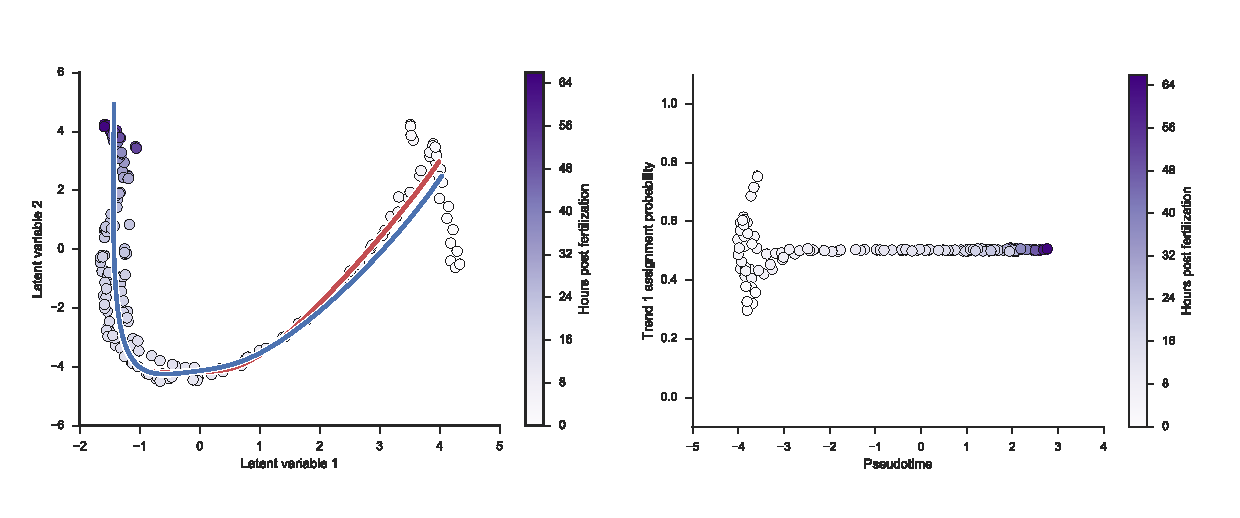
\includegraphics[width=0.95\textwidth]{frog-illustration.pdf}
    \caption{Summary of GPfates result of Owens et al developing frog embryo data.}
    \label{fig:owens}
\end{figure}

No strong bifurcation is detected, and thus we skipped gene bifurcation analysis. The single-trend model explains the data well. Some heterogeneity can be seen in the early part of the time course. This might suggest that expression is somewhat noisy in extremely early embryos, but not in a way that indicates discrete cell populations.

\section{Comparison to other pseudotime and bifurcation methods}

We compared GPfates with various methods inferring pseudotime and bifurcation events: Wishbone \cite{Setty2016-ie}, Monocle2\footnote{http://cole-trapnell-lab.github.io/monocle-release/articles/v2.0.0/}, Diffusion Pseudotime \cite{Haghverdi2016-tm}, SCUBA \cite{Marco2014-rf} and Mpath \cite{Chen2016-ar}. We applied the methods to our data and different public developmental data sets mentioned earlier. Please note, the developmental embryonic frog data was treated as a negative control to investigate if methods are able to detect false positives, i.e. identifying branches when they do not exit.

\begin{figure}
    \centering
    \includegraphics[width=0.8\textwidth]{"results_malaria"}
    \caption[Output of bifurcation methods applied to malaria data]{\textbf{Output of bifurcation methods applied to malaria data.} (A) Wishbone results showing the branching structure colored by time points (left) and inferred branches (right). (B) Minimum spanning tree on cells generated by Monocle2. Cells are colored by time points (left) and inferred cell states (right). (C) Visualisation of diffusion maps in DPT colored by time points (left) and inferred branches (right). (D) Lineage tree by SCUBA reports no bifurcation. Sizes of bubbles are according to number of cells. (E) MPath's minimum spanning tree: First number corresponds to the collection time, second number corresponds to the landmark cluster. (F) GPfates trajectory, colored by time points.}
    \label{fig:res_malaria}
\end{figure}

\begin{figure}
    \centering
    \includegraphics[width=0.8\textwidth]{"results_lung"}
    \caption[Output of bifurcation methods applied to lung data]{\textbf{Output of bifurcation methods applied to lung data.} AT2 and E18.5 cells are expected to occur in one branch. (A) Wishbone's branching structure. Cells are colored by time points (left) and inferred branches (right). (B) Minimum spanning tree generated by Monocle2. Cells are colored by time points (left) and inferred cell states (right). (C) Visualization of diffusion maps in DPT colored by time points (left) and inferred branches (right). (D) Lineage tree by SCUBA: Sizes of bubbles are according to number of cells. (E) MPath's minimum spanning tree: First number corresponds to the collection time, second number corresponds to the landmark cluster. (F) GPfates trajectory, colored by time points.}
    \label{fig:res_lung}
\end{figure}

\begin{figure}
    \centering
    \includegraphics[width=0.8\textwidth]{"results_pgc"}
    \caption[Output of bifurcation methods applied to primordial germ cell data]{\textbf{Output of bifurcation methods applied to primordial germ cell data.} Bifurcation event is expected to split female and male cells. (A) Wishbone results colored by time points (left), sex (middle) and inferred branches (right). (B) Monocle2 results colored by time points (left), sex (middle) and inferred cell states (right). (C) DPT results colored by time points (left), sex (middle) and inferred branches (right). (D) SCUBA result: Sizes of bubbles are according to number of cells. (E) MPath result: First number corresponds to the collection time, second number corresponds to the landmark cluster. (F) GPfates trajectory, colored by time points. Squares corresponds to male, triangles to female cells.}
    \label{fig:res_pgc}
\end{figure}

\begin{figure}
    \centering
    \includegraphics[width=0.8\textwidth]{"results_frog"}
    \caption[Output of bifurcation methods applied to developing frog data]{\textbf{Output of bifurcation methods applied to developing frog data.} Treated as a negative control, no branching events should be reported. Please note, Mpath failed to model on developmental frog data. (A) Wishbone results colored by time points (left) and inferred branches (right). (B) Monocle2 results colored by time points (left) and inferred cell states (right). (C) DPT results colored by time points (left) and inferred branches (right). (D) SCUBA result: Sizes of bubbles are according to number of cells. (E) GPfates trajectory, colored by time points.}
    \label{fig:res_frog}
\end{figure}

The results are summarized in Fig. \ref{fig:res_malaria} through \ref{fig:res_frog}. In order to validate the approaches, we counted the number of bifurcation events for each method in each data set and compared it to the expected number of bifurcations (Table \ref{tab:alternatives_out}).

\begin{figure}
    \centering
    \includegraphics[width=\textwidth]{"realtime_vs_pseudotime_accuracy"}
    \caption[Accuracy of bifurcation methods]{\textbf{Accuracy of bifurcation methods.} Spearman's rank correlation was calculated by comparing the real time and the inferred pseudotime.}
    \label{fig:real_vs_pseudo}
\end{figure}

Furthermore, we assessed the accuracy of a method by calculating Spearman's rank correlation between the inferred pseudotime and the real time in a given data set (Supp. Comp. Fig \ref{fig:real_vs_pseudo}). For this analysis only Wishbone, Monocle2 and DPT could be considered as the SCUBA and Mpath tools do not report an inferred pseudotime which can be parsed.

Monocle2 and GPLVM perform similarly with a high accuracy ($>$ abs(0.80) Spearman's correlation) on public data. However, Monocle2 as well as Wishbone and DPT failed to assign the correct temporal order with regard to the malaria infection data. Overall, applying Wishbone and DPT to the data sets they achieved poor to moderate accuracy, except for Wishbone performing well on the frog data, and DPT performing well on developmental lung data.

Concerning the bifurcation event in developing lung data, most of the methods cluster AT2 and E18.5  cells into one branch which has been confirmed in a previous study \cite{Treutlein2014-rz}. However, in primordial germ cell data none of the published methods were able to detect branching  events between male and female cells. With regard to the frog embryonic development study only SCUBA reflects the non-branching structure of the data. All other public methods report a branching point.

\subsection{Preprocessing public RNA-seq data}

We removed ERCCs from our expression data table and re-scaled the expression values to TPM. Furthermore, we eliminate cells containing NA's in the frog data.

Some of the used methods require a start or root cell. Therefore, We randomly picked a cell from an early collection time point: \texttt{1771-026-187-E6} (malaria), \texttt{SRP033209\_E14.5\_rep\_1\_cell\_24} (lung), \texttt{2013600} (pgc) and \texttt{1795679} (frog).

\subsection{Wishbone}

The analysis with Wishbone version 0.4.1 was performed according to the tutorial using default or suggested parameters \cite{Setty2016-ie}. We ran t-SNE with \texttt{n\_components = 5} and \texttt{perplexity = 30}. To run wishbone the start cells were chosen as  stated above with \texttt{k=15} or \texttt{k=50} for frog data, \texttt{components\_list=[1,2]} and \texttt{num\_waypoints = 150}.

\subsection{Monocle}

The Monocle analysis was performed with version 2.1.0 of the Monocle package, following the steps outlined in the original vignette \cite{Trapnell2014-cn}. In brief, the analysis was  performed using the size normalized data (TPM) including all genes expressed in $ \geq $ 50 cells with default parameters. The genes used for the ordering of cells were defined by carrying out a differential expression analysis of the time points using the \texttt{differentialGeneTest} in the \texttt{Monocle} package. Following the original vignette, genes with q-value $<$ 0.01 were selected. To reduce the dimension the \texttt{max\_components} option was set to 2 and the \texttt{DDRTree} methods was used.

\subsection{Diffusion Pseudotime (DPT)}

DPT analysis was done using the R package version \texttt{0.6.0} and an additional package called \texttt{destiny} (version \texttt{1.3.4}) ({\it 21}). In order to calculate the transition matrix DPT uses a Gaussian kernel with parameter \texttt{sigma}. The optimal \texttt{sigma} was chosen by  using the function \texttt{find.sigmas()} of the \texttt{destiny} package. Given the transition matrix and root cell \texttt{dpt()} was executed with \texttt{branching=TRUE}.

\subsection{SCUBA}

In order to run SCUBA we used the python package \texttt{PySCUBA} version  \texttt{0.1.1}\footnote{https://github.com/GGiecold/PySCUBA} which provides a graphical user interface \cite{Marco2014-rf}. Selecting the RNA-seq data set including temporal information we ran SCUBA with  \texttt{cluster\_mode = PCA2} and \texttt{pseudotime\_mode = 0}.

\subsection{Mpath}

We performed analyses with Mpath using the package version \texttt{1.0} \cite{Chen2016-ar}. Prior to the analysis, a quality check includes a removal of genes having TPM values $ < $ 1 in more than 95 percent of cells in each group. In order to find the number of optimal clusters the parameters \texttt{diversity\_cut} and \texttt{size\_cut} were set as suggested to 0.6 and 0.05, respectively, when calling the function \texttt{landmark\_designation()}. Inspecting the resulting plots, the number of optimal clusters were chosen as 10 (malaria), 19 (lung) and 24 (pgc). Mpath failed to run on the frog data set. Using the landmark clusters we constructed the weighted neighborhood graph and trimmed it using the minimal spanning tree method. 

\section{Discussion}

We have demonstrated the applicability of our GPfates method, where we use latent variable modeling to infer temporal expression dynamics, and Gaussian process mixture modeling for identifying diverging global trends. The method has been investigated in terms of robustness, and applied on several simulated and real data sets showing good results.

Of course there is no silver bullet for these sorts of problems, and it would not be surprising if other methods than the ones we have used work better for some biological systems. Nevertheless, we have illustrated that the main component, the Gaussian process mixture modeling, is compatible with other methods in these cases.

A benefit from the methods we use is that diagnostics such as marginal likelihood can be used to aide the user with regards to the models to use. Still, the user will need to keep the biological system in mind, and be critical of results.

\begin{table*}
\centering
\begin{tabularx}{0.95\textwidth}{lll}
\textbf{Pseudotime Method} & \textbf{Strategy} & \textbf{OMGP Compatibility} \\
\hline \\ 
Wishbone & Diffusion maps on reduced k-NN & Yes \\
({\it 22}) & graph (using waypoints) & \\ & & \\
Monocle2 Pseudotime &  Minimum Spanning Tree path length & Yes \\
({\it 19}) & in 2D DDRTree space &  \\ & &  \\
Diffusion maps & Spectral embedding of data manifold & With postprocessing, e.g. DPT \\
({\it 56}) & & ({\it 21}) \\ & & \\
Wanderlust & Heuristic k-NN graph geodesic distance & Yes \\
({\it 36}) & & \\ & & \\
GPLVM & Latent data parametrization & Yes  \\ & & \\
\end{tabularx}
\begin{tabularx}{0.95\textwidth}{lllll}
 &  & \textbf{Dim. } & \textbf{Clus-} & \textbf{Diff. Expr.} \\
\textbf{Bifurcation Method} & \textbf{Strategy} & \textbf{Reduction} & \textbf{tering} & \textbf{Analysis} \\
\hline \\
Wishbone & Disagreements between shortest paths & Yes & No & No \\
({\it 22}) & & & & \\ & & & &\\
Monocle2 states & Create k PQ trees from a Minimum & Yes & No & Yes \\
({\it 19}) & Spanning Tree & & & \\ & & & &\\
DPT & Switch in correlation behavior & No & No & No \\
({\it 21}) & & & & \\  & & & & \\
SCUBA & Transitions between clusters in pseudo-& Yes & Yes & No \\
({\it 18}) & time bins & & & \\  & & & & \\
Mpath & Finding Minimum Spanning Tree in & Yes & Yes & Yes \\
({\it 20}) & neighborhood graph of landmarks &  & &  \\ & & & & \\
OMGP & Model data as mixture of continuous& Yes & No & No \\
& processes & & & \\
\end{tabularx}
\caption{Examples of common pseudotime- and bifurcation methods.}
\label{tab:alternatives}
\end{table*}

\begin{table*}
\centering
\begin{tabularx}{0.95\textwidth}{lllll}
 & \textbf{Malaria} & \textbf{Lung} & \textbf{PGC} & \textbf{Frog} \\
 & \textbf{this work} & ({\it 23}) & ({\it 24}) & ({\it 64}) \\
\hline \\ 
Wishbone & 1 (1) & 1 (1) & 1 (1) & 1 (0) \\
Monocle2 & 7 (1) & 1 (1) & 2 (1) & 1 (0) \\
DPT & 1 (1) & 0 (1) & 1 (1) & 1 (0) \\
SCUBA & 0 (1) & 0 (1) & 0 (1) & 0 (0) \\
Mpath & 1 (1) & 2 (1) & 1 (1) & NA (0) \\
\end{tabularx}
\caption{Number of detected (and expected) bifurcations of other methods.}
\label{tab:alternatives_out}
\end{table*}

%*******************************************************************************
%****************************** Fifth Chapter **********************************
%*******************************************************************************

\chapter{Detecting spatially dependent genes in spatial expression assays} \label{ch:spatial}

\graphicspath{{Chapter5/Figs/}}

Technological advances have enabled low-input RNA-sequencing, paving the way for assaying transcriptome variation in spatial contexts, including in tissue systems. While the generation of spatially resolved transcriptome maps is increasingly feasible, computational methods for analysing the resulting data are not established. Existing analysis strategies either ignore the spatial component of gene expression variation, or require discretization.

To address this, we have developed \name{SpatialDE}, a computational framework for identifying and characterizing spatially variable genes. Our method generalises variable gene selection, as used in population- and single-cell studies, to spatial expression profiles. We apply \name{SpatialDE} to Spatial Transcriptomics and to data from single cells expression profiles using multiplexed In Situ Hybridisation (SeqFISH and MERFISH), demonstrating its general use. \name{SpatialDE} identifies genes with expression patterns that are associated with histology in breast cancer tissue, several of which have known disease implications and are not detected by variable gene selection. Additionally, our model can be used to classify genes with distinct spatial patterns, including periodic expression profiles, linear trends and general spatial variation.

This chapter takes the concepts introduced in Chapter \ref{ch:zebrafish} and reworks them in a spatial context, rather than a temporal. Here we also formalize the statistics of the significance test, and provide computational speedups. The analysis in Chapters \ref{ch:zebrafish} and \ref{ch:malaria} had to be run on hundreds of compute nodes to finish within reasonable time frames. In the work presented in this chapter the analyses were reproduced in just a few minutes, on a standard desktop computer.

First we present the motivation and results of our analysis of public data using our method. Following this, we present the model in detail.

\section{Results}

Technological advances have helped to miniaturize and parallelize genomics, thereby enabling high-throughput transcriptome profiling from low quantities of starting material, including in single cells. Increased experimental throughput has also led to new experimental designs, where the spatial context of gene expression variation can now be assayed directly. This is critical for decoding complex tissues from multicellular organisms. The spatial context of gene expression is crucial in determining the functions and phenotypes of cells \cite{Ledford2017-hq, Lee2017-om}. In many cases a gene’s expression is determined by cellular communication and in other cases cells migrate to specific locations in tissue to perform their functions.

Several experimental methods to measure gene expression levels in a spatial context have been established, which differ in resolution, accuracy and throughput. These include the computational assignment of transcriptome-profiles from dissociated cells to a spatial reference \cite{Achim2015-fe, Satija2015-lz}, parallel profiling of mRNA using barcodes on a grid of known spatial locations \cite{Junker2014-do, Chen2017-lg, Stahl2016-ym}, and methods based on multiplexed in situ hybridization \cite{Shah2016-bi, Moffitt2016-bi} or sequencing \cite{Ke2013-ek, Lee2014-ix, Lee2015-sz}.

A first critical step in the analysis of the resulting datasets is to identify the genes that exhibit spatial variation across the tissue. However, existing approaches designed to identify highly variable genes \cite{Brennecke2013-vv, Vallejos2015-fh}, in e.g. single-cell RNA-sequencing (scRNA-seq) studies, ignore the spatial location and do not measure spatial variability. Alternatively, researchers have applied ANOVA to test for differential expression between groups of cells, either derived using a priori defined (discrete) cell annotations or based on clustering \cite{Achim2015-fe, Satija2015-lz, Stahl2016-ym, Shah2016-bi, Ke2013-ek}, with some clustering strategies incorporating spatial information \cite{Pettit2014-pa}. Importantly, such strategies are unable to detect variation that is not well captured by discrete groups, including linear and nonlinear trends, periodic expression patterns and other complex patterns of expression variation. 

\begin{figure}
    \centering
    \includegraphics[width=0.6\textwidth]{"Figure 1"}
    \caption[Overview of \name{SpatialDE} for the identification of spatially variable genes]{\textbf{Overview of \name{SpatialDE} for the identification of spatially variable genes} (A)  In spatial gene expression studies, expression levels vary in ways that depend on spatial coordinates. \name{SpatialDE} defines spatial dependence for a given gene using a non-parametric approach, testing whether gene expression levels at different locations covary in a manner that depends on their relative location. (B) \name{SpatialDE} partitions the expression variation into a spatial component (using functional dependencies \( f((x_1, x_2)) \)), characterized by alternative spatial covariances, and observation noise (\( \Psi \)). Alternative spatial covariance models considered by \name{SpatialDE}: no spatial effect (null model), general spatial, periodic spatial patterns and linear trends. Example expression patterns with the covariances plotted below corresponding matrix. (C) Computational efficiency of \name{SpatialDE} compared to a \name{Stan} implementation of the same model. Caching operations and linear algebra speedups are used where possible, enabling genome-wide analyses with thousands of samples. Benchmarks performed on a late 2013 iMac with 3.2 GHz Intel Core i5 processor.}
    \label{fig:spatialde}
\end{figure}

To address this, we propose a computational approach termed \name{SpatialDE} for identifying and characterizing spatially variable genes (SV genes). Our method builds on Gaussian Process Regression, a class of models that is widely used in geostatistics, also known as Kriging \cite{Williams2006-kb}. For each gene, our model decomposes the expression variability into a spatial and non-spatial component (Figure \ref{fig:spatialde}A). Significant SV genes can then be identified by comparing this full model to a model that assumes no spatial dependency of expression variation (Figure \ref{fig:spatialde}B, Methods).

In addition to identifying spatially variable genes, \name{SpatialDE} also allows to classify the spatial patterns of individual genes, differentiating between linear trends, periodic expression profiles or general spatial dependencies (Figure \ref{fig:spatialde}B). By interpreting the fitted model parameters it is possible to identify the length scale (the expected number of changes directional in a unit interval \cite{Williams2006-kb}) or the period length of spatial patterns for individual genes (Figure \ref{fig:spatialde}B). Finally, \name{SpatialDE} achieves unprecedented computational efficiency by leveraging computational tricks for efficient inference in linear mixed models \cite{Lippert2011-fm} and precomputing operations where possible (Figure \ref{fig:spatialde}C). Taken together, \name{SpatialDE} is a widely applicable tool for the initial analysis of spatial transcriptomics datasets.

\begin{figure}[b!]
    \centering
    \includegraphics[width=0.95\textwidth]{"Figure 2"}
    \caption[Applications of \name{SpatialDE} to Spatial Transcriptomics and data generated using SeqFISH]{(Caption on next page)}
    \label{fig:spatialresult}
\end{figure}
\addtocounter{figure}{-1}
\begin{figure} [t!]
    \caption[Applications of \name{SpatialDE} to Spatial Transcriptomics and data generated using SeqFISH]{\textbf{Applications of \name{SpatialDE} to Spatial Transcriptomics and data generated using SeqFISH.} (A) Correlated image of breast cancer tissue from Spatial Transcriptomics \cite{Stahl2016-ym}. (B) Visualization of nine selected spatially variable genes (out of 115, FDR < 0.05). The black scale bar corresponds to 1 mm. For genes identified with periodic dependencies, the orange bar shows the fitted period length on the same scale. Analogously, the blue bar shows the fitted length scale for genes with general spatial trends. 2D plots show the relative expression level for genes across the tissue section coded in color. Stars next to gene names denote significance levels (* \( q \)-value < 0.05 , ** \( q \)-value < 0.01, *** \( q \)-value < 0.001) of spatial variation. Insets in lower left show the posterior probability of these three function classes for each gene. (C) Proportion of variance (x-axis) explained by spatial variation (FSV) versus adj. P-value (y-axis, FDR adjusted) for 12,856 genes. Dashed line corresponds to the FDR = 0.05 significance level (N = 115 genes). Genes classified as periodically variable are shown in orange (N = 22), genes with a general spatial dependency in blue (N = 93). Disease-implicated genes annotated based on prior knowledge \cite{Stahl2016-ym} are indicated with red labels, and are significantly enriched in \name{SpatialDE} results (\( P = 10^{-11} \), Fisher exact test). Other representative genes selected by stratifying over function periods / length scales are annotated with black labels. Size of of points indicate certainty in the estimate of Fraction Spatial Variance (FSV), larger points have smaller standard deviation. The X symbol show the result of running \name{SpatialDE} on the estimated total RNA content per spot. (D) SeqFISH data from a region of mouse hippocampus from Shah et al \cite{Shah2016-bi}. Black scale bar correspond to 50 \( \mu \)m, Voronoi tessellation representative of tissue structure. (E) Expression patterns of six selected SV genes analogous to panel B (out of 32, FDR < 0.05). Shown are genes with linear (htr3a ), periodic (foxj1 ), and generally spatial models. Black arrows indicate distinct region of low expression of  Mog ,  Myl14  and  Ndnf. (F) Proportion of variance (x-axis) versus adj. P-value (y-axis, FDR adjusted) for 249 genes, as in (C). Genes with a linear dependency are highlighted in green.}
\end{figure}

First, we applied our method to Spatial Transcriptomics (ST) data from breast cancer tissue \cite{Stahl2016-ym}. Briefly, ST gene expression levels are derived from thin tissue sections of frozen material, placed on an array with poly(dT) probes and spatially resolved DNA barcodes in a grid of “spots”. Following permeabilization, the mRNA is captured by the probes, and the spatial location can be recovered from sequenced barcodes. The resulting gene expression profiles can be analysed in the context of hematoxylin and eosin (HE) stained microscopic images of the tissue (Figure \ref{fig:spatialresult}A).

\name{SpatialDE} identified 115 SV genes (FDR < 0.05). Notably, seven highly ranking genes were also included in a set of 14 genes with known roles in the disease that were highlighted in the primary analysis of the data (Figure \ref{fig:spatialresult}C, red text). Significantly SV genes were enriched for collagens, which distinguish tissue substructure \cite{Seewaldt2012-lk} (Reactome term “Collagen formation”, P < 5 * 10-14 using gProfiler \cite{Reimand2016-nz}). Additionally, we identified the autophagy related gene, TP53INP2, surrounding the fatty tissue (\( q \)-value = 0.022, Figure \ref{fig:spatialresult}B, extended examples Figure \ref{fig:ss1}). Interestingly, the set of SV genes also included the cytokines CXCL9 (\( q \)-value = 5.4 * 10-4) and CXCL13 (\( q \)-value = 1.3 * 10-4), both of which are expressed in a visually distinct region (Figure \ref{fig:spatialresult}A, black arrow), together with the IL12 receptor subunit gene IL12RB1 (\( q \)-value = 2.8 * 10-4), indicating a potential tumour related immune response in the tissue. Notably, neither of these genes (and N=29 others), were identified as differentially expressed when applying clustering in conjunction with an ANOVA test between the identified groups of cells (Figure \ref{fig:ss2}). Nor did they have highly ranked based on conventional Highly Variable Genes measures (such as the mean-\( \text{CV}^2 \) relation \cite{Brennecke2013-vv} or mean-dropout rate relation \cite{Andrews2016-ky}); measures that do not take the spatial context into account (Figure \ref{fig:ss3}). Generally, we observed that \name{SpatialDE} is complementary to existing methods, and is able to find SV genes with localized expression patterns, as indicated by small fitted length scales, or periodic patterns, that are not detected by methods that ignore spatial contexts (Figure \ref{fig:ss2}E). Finally, we confirmed the statistical calibration and the robustness of \name{SpatialDE} using randomization experiments (Figure \ref{fig:ss4}). 

As a second application, we considered a study of mouse olfactory bulb \cite{Stahl2016-ym}, profiled using the same ST protocol. Again, \name{SpatialDE} identified SV genes with clear spatial sub-structure, consistent with the matched HE stained image (Figure \ref{fig:ss5}A-B). These included canonical marker genes highlighted in Stahl et al, such as PENK, DOC2G, and KCTD12, but also additional genes that define the granule cell layer (GCL) of the bulb. Genes in the latter set were classified as periodically variable with period lengths corresponding to the distance between the centers of the hemispheres (including KCNH3, NRGN, or MBP with 1.8 mm period length, Figure \ref{fig:ss5}). Other genes with periodic patterns, such as the vesicular glutamate transporter SLC17A7, were identified with shorter periods (1.1 mm), and inspection revealed regularly dispersed regions, potentially identifying a pattern with regions of higher neuron density \cite{Jahn2000-yw}. This suggests that periodic expression patterns in tissue contexts are a biological feature of interest.

Taken together, these results demonstrate that \name{SpatialDE} can be used to characterize clinically relevant features in spatial tissue samples in the absence of \textit{a priori} histological annotation.

\name{SpatialDE} is not limited to sequencing technologies, and can be applied to any expression datatype with spatial and/or temporal resolution. To explore this, we applied the method to data generated using multiplexed single molecule FISH (smFISH), a recent technological development that allows for quantifying gene expression with subcellular resolution for large numbers of target genes in parallel. Briefly, probes are hybridized to RNA while carrying barcodes of fluorophores, which allows for quantifying gene expression using several thousand probes \cite{Chen2015-rm} by high-content imaging.

We applied \name{SpatialDE} to Multiplexed smFISH data from mouse hippocampus, generated using SeqFISH \cite{Shah2016-bi}. This study considered 249 genes that were chosen to investigate the cell type composition along dorsal and ventral axes of the hippocampus (Figure \ref{fig:spatialresult}D). \name{SpatialDE} identified 32 SV genes (FDR < 0.05), with the three highest ranking genes, MOG (\( q \)-value \( = 10^{-14} \)), MYL14, (\( q \)-value = \( 10^{-14} \)) and NDNF (\( q \)-value \( = 2 \cdot 10^{-12} \)) displaying a distinct region of lower expression (Figure \ref{fig:spatialresult}E, black arrows). Again, \name{SpatialDE} identified genes with different types of spatial variation, including linear trends (N=5) and periodic patterns (\( N = 8 \), Figure \ref{fig:spatialresult}F, extended examples in Figure \ref{fig:ss6}).

\name{SpatialDE} can also be used to test for spatial expression variation in cell culture systems, where spatial variation may not be expected a priori. We explored this, and considered data from another recent multiplexed smFISH dataset generated using MERFISH with 140 probes from a human osteosarcoma cell culture \cite{Moffitt2016-bi} (Figure \ref{fig:ss7}A-B). Interestingly, the model revealed that a substantial proportion of the genes assayed were spatially variable (N=92, 65\%, FDR < 0.05). This reconstitutes results from the primary analysis, where the authors noted spatially restricted populations of cells with higher proliferation rates. Indeed, six of the seven genes highlighted as differentially expressed between proliferation subpopulations were identified as SV genes (e.g. THBS1 and CENPF1, Figure \ref{fig:ss7}C). This result is also consistent with previous studies which observed that high confluence in cell culture, promoting cell-to-cell communication and causing crowding, leads to spatial dependency in gene expression \cite{Battich2015-qu}. We also considered negative control probes in the data, which were not detected as spatially variable, thereby confirming the statistical calibration of \name{SpatialDE} (Figure \ref{fig:ss7}D).

\section{Discussion}

Herein, we have presented a method for identifying spatially variable genes. The commoditization of high-throughput experiments, including spatially resolved RNA-seq, means that there will be a growing need for methods that account for this new dimension of expression variation, such as \name{SpatialDE}.

We applied our model to data from multiple different protocols, from Spatial Transcriptomics to multiplexed single-molecule FISH, considering both tissue systems and cell lines. The extent of spatial variation we observed in cell lines may be surprising, a result that is consistent with recent studies that have reported coordinated expression changes across neighbouring cells \cite{Battich2015-qu}. The method is also applicable to temporal data from time-course experiments (Figure \ref{fig:ss8}), and it can be applied without modification to 3-dimensional data from e.g. in situ sequencing when such technologies mature \cite{Lee2014-ix, Lee2015-sz}.

\name{SpatialDE} generalizes previous approaches for the detection of highly variable genes, most notably methods designed for conventional scRNA-seq \cite{Brennecke2013-vv}. Our model separates spatial variation from non-spatial effects, which may include biological and technical variability. Underlying this approach is the assumption that technical noise is independent across sampling positions, which circumvents the need to explicitly model technical sources of variation, which enables applications to virtually any protocol.

Future extension of \name{SpatialDE} could be tailored towards specific platforms, for example to make use of spike-in standards or unique molecular identifiers, thereby explicitly estimating technical variation. Another area of future work are extensions for incorporating information about the tissue makeup or local differences in cell density. Our framework also opens up the possibility for future work to define spatial patterns that are common to groups of genes, using clustering combined with the spatial Gaussian Process framework \cite{Hensman2015-op}.

\section{The \name{SpatialDE} model}

\name{SpatialDE} builds on the Gaussian process framework which we introduced in Section \ref{sec:pseudotime-model}, thereby assessing the evidence that the gene expression patterns of individual genes are explained by functions with different spatio-temporal dependencies.

In the following we assume that $ \bfy = (y_1,\dots,y_N) $ corresponds to a vector of expression values at $N$ spatial locations $ \bfX = (\bfx_1,\dots,\bfx_N) $ for a given gene.  The coordinates of the spatial locations are typically two-dimensional, i.e. $ \bfx_i = (x_{i_1}, x_{i_2}) $, however the model is general and can also be applied to any dimensionality such as three-dimensional or uni-dimensional (e.g. time-series) data. 

\subsection{Gaussian Processes regression}

A Gaussian Process (GP) is a probability distribution over functions $ y = f(\bfx) $,
\begin{align}
 f \sim \GP(k\left(\bfx,\bfx' \given \btheta\right)). 
\end{align}
A Gaussian process model $ \GPM $ is defined by the covariance function $ k(\bfx,\bfx' \given \btheta) $, which parameterizes the dependency between any pair of function values based on their inputs $ \bfx $ and $ \bfx' $; and $ \btheta $ denotes a vector of additional hyperparameters of the covariance (see below). 

Any finite representation of a GP for an observed dataset can be obtained by marginalizing over all unobserved function values, resulting in a finite realisation of joint Gaussian distribution: 
\begin{align}
\label{eq:GP}
p(\bfy \given \GPM) =  \normal{\bfy}{\mu {\bf 1}, \sigma_s^2 \cdot \left ( \bSigma_{k(\bfx,\bfx'\given \btheta)} + \delta \cdot \unit \right )}.
\end{align}
Here, $ \mu \bf 1 $ account for mean effects (bias term) and the scaling parameter $ \sigma_s^2 $ determines the proportion of variance explained by the spatial covariance. The term $ \sigma_s^2 \delta \unit $ explains iid observation noise, i.e. variation in the data that does not follow the spatial pattern.

The covariance matrix is derived by evaluating the covariance function for all pairs of observed datums $ {\bSigma_{k(\bfx,\bfx'\given \btheta)}}_{i,j} $ = $ k(\bfx_i,\bfx_j \given \btheta)$, for which the parameters $\btheta$ can be determined using maximum likelihood (see Secion~\ref{sec:param_inference}).

\begin{align}
\label{eq:LML}
\hat{\btheta} =& \argmax_{\btheta} LL(\GPM, \btheta) \\
              =& \argmax_{\btheta} \log p(\bfy \given \GPM,\btheta), \nonumber
\end{align}
where $LL(\GPM, \btheta)$ denotes the log marginal likelihood.

\subsection{Covariance functions}
\label{sec:covariance_functions}
To test and compare between alternative hypothesis of spatial variation of expression patterns, we assess GP models with different covariance functions.
\begin{itemize}
\item Null model \\
$k_{\text{null}}(\bfx,\bfx')\propto 0$\\
\item General spatial pattern (known as the \textit{RBF} or \textit{Gaussian kernel}) \\
$k_{\text{spatial}}(\bfx,\bfx' \given \btheta) \propto e^{ {-\frac{1}{2L^2} | \bfx-\bfx' |^2}}$\\
\item Linear trend \\
$k_{\text{lin}}(\bfx,\bfx' \given \btheta) \propto \bfx{\bfx'}^{\T}$\\
\item Periodic pattern (known as the \textit{cosine kernel}) \\
$k_{\text{periodic}}(\bfx,\bfx' \given \btheta) \propto \cos({\frac{1}{p} | \bfx-\bfx' |})$
\end{itemize}

\subsubsection*{Interpretation of model parameters}

As the scale is parameterized using $ \sigma_s^2 $ in Eq.~\ref{eq:GP}, the proportionality factors do not change the marginal likelihood. However, in order to be able to interpret the parameter $ \sigma_s^2 $ as the proportion of variance explained we use Gower's transformation to correct the $ \sigma_s^2 $ parameter for the structure in the covariance matrix $ \bSigma $~\cite{Kostem2013-gm}:
\[
g = \frac{\Tr (P \bSigma P)}{n - 1},
\]
where
\[
P = I - \frac{1}{n} {\bf 1} {\bf 1}^{\T}.
\]

This allows for defining the Fraction of Spatial Variance, $ \text{FSV} = \frac{\sigma^2_s \cdot g}{\sigma^2_s \cdot g + \sigma^2_s \cdot \delta} $, which corresponds to the proportion of varaince explained by the spatial variance component compared to the total variance.

\subsection{Statistical significance and classification of spatially variable genes}

\subsubsection*{P-values from hypothesis testing}

Significant spatial variance component are tested via mode comparison: 
\begin{align*}
    p(\bfy \given \model_1) &=  \normal{\bfy}{\mu {\bf 1}, \sigma_s^2 \cdot \left ( \bSigma_{k(\bfx,\bfx'\given \btheta)} + \delta \cdot \unit \right )}, \\
    p(\bfy \given \model_0) &=  \normal{\bfy}{\mu {\bf 1},  \sigma_s^2 \cdot \unit}.
\end{align*}

Here, $\model_1$ denotes the alternative model that includes both a spatial and non-spatial component and $\model_0$ denotes the null model, lacking a spatial variance component.

The parameters of both models are optimised using maximum likelihood (see Section~\ref{sec:param_inference}).
Significance of the spatial variance component is then assessed using a likelihood ratio test (LRT) between the alternative and the null model. 
P-values can be estimated in closed form, assuming that the log likelihood ratios (LLRs) under the null model are \( \chi^2 \) distributed with one degree of freedom.

\begin{sloppypar}
To correct for multiple testing, we use the FDR based strategy by~\cite{Storey2003-ap} yielding \( q \)-values.  Unless stated otherwise, we report genes at \( q \)-Value \( < 0.05 \) as significant SV genes.
\end{sloppypar}

Calibration of the P-values was investigated through negative control probes in the MERFISH experiment. The fraction of significant negative control probes behave as expected with regards to the family-wise error rate (Figure \ref{fig:ss7}).

\subsubsection*{Classification of spatial patterns using model comparison}

In order to identify interpretable spatial trends, we can compare the spatial model to alternative models that make stronger assumptions about the spatial dependency. 
Specifically, for significant spatially variable genes (e.g. \( q \)-value \( < 0.05 \)), we compare GP models with alternative prior covariances: the general spatial model using an RBF kernel, a GP prior with periodic covariance function, using the cosine kernel (See Section~\ref{sec:covariance_functions}), and a GP prior with linear covariance function.

As these models differ in their number of parameters, we employ the Bayesian Information Criterion (\( BIC \)), which has been shown to be effective for model comparisons of alternative GP models~\cite{Lloyd2014-ky}. The BIC penalises the maximum log-likelihood by the number of effective parameters in the model, thereby accounting for differences in model complexity:
\[
BIC = \log (n) \cdot M - 2 \cdot \hat{LL}.
\]
Here, \( \hat{LL} \) denotes the log marginal likelihood (Eq.~\ref{eq:LML}), $ M $ corresponds to the number of observations and $n$ denotes the number of hyperparameters of a given model. Each gene is then classified into different spatial trends by selecting the GP model that minimises the \( BIC \).

We also use the \( BIC \) to estimate posterior probabilities of specific models. Briefly, the \( BIC \) is an estimate of \( -\log p( \bfx, \bfy | \mathcal{H}_i ) \), which allows for deriving an approximate form of the marginal likelihood of the model \( \mathcal{H}_i \),
\[
p( \mathcal{H}_i | \bfX, \bfy) = \frac{1}{Z} \cdot p(\bfX, \bfy | \mathcal{H}_i) \cdot p( \mathcal{H}_i ) = \frac{1}{Z} \cdot \int_{\theta} p( \bfX, \bfy | \mathcal{H}_i, \theta ) d \theta \approx -\frac{1}{Z} \cdot BIC_i, 
\]
where
\[
Z = \sum_i p(\bfX, \bfy | \mathcal{H}_i) \cdot p( \mathcal{H}_i ) \approx \sum_i -BIC_i.
\]
We consider the models \( \{ \mathcal{H}_{\text{spatial}}, \mathcal{H}_{\text{linear}}, \mathcal{H}_{\text{periodic}} \} \) described above (Section~\ref{sec:covariance_functions}), deriving posterior probabilities of these models given the data.


\subsection{Parameter inference}
\label{sec:param_inference}

Maximum likelihood inference (Eq.~\ref{eq:LML}) requires determining $ \mu $, $ \sigma_s^2 $, $ \delta $ and, depending on the model, additional hyperparameters of the selected covariance function (e.g. the length-scale $l$, see Section~\ref{sec:covariance_functions}). The log likelihood is 
\begin{align*}
LL(\bfy, \bfX, \theta) =  -\frac{1}{2} \left( \right. &n \log (2 \pi) + \log (|\sigma_s^2 \cdot (\bSigma_\ell + \delta \cdot \unit) | ) + & \\
& \left. (\bfy - \mu)^T (\sigma_s^2 \cdot (\bSigma_\ell + \delta \cdot \unit ) )^{-1}  (\bfy - \mu) \right) &
\end{align*}

Evaluation of the likelihood requires inverting the covariance matrix \( \bSigma_\ell \) which depends on the parameter \( \ell \), this makes gradient based optimisation of \( \ell \) a key bottleneck in inference. We comment on this later, but for now, assume \( \ell \) is known. To circumvent inverting the entire matrix \( \sigma_s^2 \cdot (\bSigma_\ell + \delta \cdot \unit )  \), we follow \cite{Lippert2011-fm} and factor the matrix \( \bSigma_\ell \) by spectral decomposition, \( USU^T = \bSigma \), and noting that \( UU^T = I \):
\begin{align*}
   \sigma_s^2 \cdot (\bSigma_\ell + \delta \cdot \unit ) =
   \sigma_s^2 \cdot (USU^T + \delta \cdot \unit ) =
   \sigma^2_{s} \cdot U (S + \delta \cdot \unit) U^T
\end{align*}

\begin{sloppypar}
Now if we write the log likelihood as a function of \( \delta, \sigma_s^2 \) and \( \mu \), we obtain
\begin{align*}
& LL(\delta, \sigma_s^2, \mu) = \\
&= -\frac{1}{2}( n \log (2 \pi \sigma_s^2 ) + \log (| \bSigma_\ell + \delta \cdot \unit |) +  \frac{1}{\sigma_s^2} (\bfy - \mu)^T (\bSigma_\ell + \delta \cdot \unit)^{-1} (\bfy - \mu)) \\
&= -\frac{1}{2}( n \log (2 \pi \sigma_s^2 ) + \log (|U(S+\delta I)U^T|) \frac{1}{\sigma_s^2} (\bfy - \mu)^T (U(S + \delta \cdot \unit)U^T)^{-1} (\bfy - \mu)) \\
&= -\frac{1}{2}( n \log (2 \pi \sigma_s^2 ) + \log (|U||S + \delta \cdot \unit||U^T|) + \frac{1}{\sigma_s^2} (\bfy - \mu)^T U (S + \delta I)^{-1} U^T (\bfy - \mu)) \\
&= -\frac{1}{2}( n \log (2 \pi \sigma_s^2 ) + \log (|S + \delta \cdot \unit|) + \frac{1}{\sigma_s^2} ((U^T\bfy) - (U^T1)\mu)^T (S + \delta \cdot \unit)^{-1} ( (U^T\bfy) - (U^T1) \mu)) \\
&= -\frac{1}{2}(n \log (2 \pi \sigma_s^2) + \sum_{i=1}^n \log (S_{i,i} + \delta) + \frac{1}{\sigma_s^2} \sum_{i=1}^n \frac{([U^T\bfy]_i - [U^T1]_i \mu)^2}{S_{i,i} + \delta})
\end{align*}
\end{sloppypar}

The key features used is that \( |U| = |U^T| = 1 \), and \( S + \delta \cdot \unit \) is diagonal, so both the determinant and inverse are trivial to compute. The expression \( U^T1 \) only depends on the coordinates \( X \) and can be precomputed for every gene.
The expression \( U^T\bfy \) will need to be re-computed for each gene, however, it can be re-used for inference evaluations.

We make use of the constraint that for the optimal \( \mu = \hat{\mu} \) we must have 
\[
\frac{\partial LL(\delta, \sigma_s^2, \mu)}{\partial \mu} = 0,
\] and so
\begin{align*}
& & \frac{1}{\sigma_s^2}( (U^T1)^T (S + \delta \cdot \unit )^{-1} (U^T\bfy) - (U^T1)^T (S + \delta \cdot \unit)^{-1} (U^T1) \hat{\mu}) = 0 \\
\Rightarrow & & \\
& & (U^T1)^T (S + \delta \cdot \unit)^{-1} (U^T1) \hat{\mu} = (U^T1)^T (S + \delta \cdot \unit)^{-1} (U^T\bfy) \\
\Rightarrow & & \\
&\hat{\mu} &= ((U^T1)^T (S + \delta \cdot \unit)^{-1} (U^T1))^{-1} (U^T1)^T (S + \delta \cdot \unit)^{-1} (U^T\bfy) \\
& &= \sfrac{\left( \sum_{i=1}^n \frac{1}{S_{i,i} + \delta} [U^T1]_i^T [U^T\bfy]_i \right)}{\left( \sum_{i=1}^n \frac{1}{S_{i,i} + \delta} [U^T1]_i^T [U^T1]_i \right)}.
\end{align*}
When data is given, this expression only depends on \( \delta \) and we write this as \( \hat{\mu}(\delta) \).

The same procedure for \( \sigma_s^2 \) gives us
\begin{align*}
    \hat{\sigma}_s^2(\delta) = \frac{1}{n} \sum_{i=1}^n \frac{([U^T\bfy]_i - [U^T1]_i \hat{\mu}(\delta))^2}{S_{i,i} + \delta},
\end{align*}
which also depend only on \( \delta \). So the entire expression for the log likelihood can be written as
\begin{align*}
    LL(\delta) &= -\frac{1}{2}( n \log (2 \pi) + S_1(\delta) + n + n \log ( \frac{1}{n} S_2(\delta))), \\
    S_1(\delta) &= \sum_{i=1}^n \log (S_{i, i} + \delta), \\
    S_2(\delta) &= \sum_{i=1}^n \frac{([U^T\bfy]_i - [U^T1]_i \hat{\mu})^2}{S_{i,i} + \delta}.
\end{align*}

To optimise \( LL(\delta) \) with respect to \( \delta \)  we use gradient based optimisation with l-bfgs-b and numerically approximated gradient. Empirically, we observed that an analytically calculated gradient would require more floating point operations per iteration step with no gain in performance.

To avoid gradient based optimization of the length scale \( \ell \), we precalculate a grid of covariance matrices \( \bSigma_\ell \) and factorise them. The number of grid points can be specified by the user, but our default settings put 10 grid points logratihmically spaced between half shortest and twice the longest distance observed in the data. We have found to give sufficient sensitivity. After factoring the \( \bSigma_\ell \)'s, the \( U \) and \( S \) matrices can be reused for each gene. We only need to do as many \( O(n^3) \) matrix inversions as we have grid points. Each gene under investigation will have a \( O(n^2) \) step for each grid point to calculate the \( U^T\bfy \) factor. All other calculations, including each optimisation iteration, will be \( O(n) \). Since our aim is to investigate data where \( G >> 10 \), this greatly reduces the computational burden, as illustrated in Figure \ref{fig:spatialde}C.

\subsubsection*{Estimation of standard errors}

The only optimised parameter in our model is \( \delta \), the uncertainty of the maximum likelihood estimate of this parameter is the inverse of \( \frac{\partial^2 LL(\delta)}{\partial \delta^2} \) evaluated at \( \hat{\delta} \). We use rules of uncertainty propagation to estimate uncertainty of \( \text{FSV} \) since this can be expressed as a function of \( \delta \),
\[
\text{FSV}(\delta) = \frac{\hat{\sigma}^2_s(\delta) \cdot g}{\hat{\sigma}^2_s(\delta) \cdot g + \delta \cdot \hat{\sigma}^2_s(\delta)},
\]
where \( g \) is the Gower factor for covariance matrix \( \bSigma_\ell \) for a given grid point. So, the standard error of \( \text{FSV} \) is
\[
s_{\text{FSV}}^2 = \left(\frac{\partial \text{FSV}(\delta)}{\partial \delta} \Bigr|_{\delta = \hat{\delta}}\right)^2 \cdot s_\delta^2,
\]
where
\[
s^2_\delta = \sfrac{1}{\left(\frac{\partial^2 LL(\delta)}{\partial \delta^2} \Bigr|_{\delta = \hat{\delta}}\right)^2}.
\]

To evaluate the two derivatives, we use finite difference approximation on the \( LL \) and \( \text{FSV} \) functions.

\section{Data normalisation}

The presented Gaussian process model is based on the assumption of normally distributed residual noise and independent observations across cells. To meet these requirements, we have identified two necessary normalisation steps.

\begin{figure}
    \centering
    \includegraphics[width=0.95\textwidth]{"anscombe-figure"}
    \caption[Variance stabilization of negative binomial counts]{\textbf{Variance stabilization of negative binomial counts.} (\textbf{A}) Mean \textit{vs} variance relation of genes in the different spatial technologies. Compared to Poisson noise, variance is higher than expected, and is consistent with negative binomial noise with a fixed overdispersion parameter per dataset. (\textbf{B}) The same figure after applying the approximate Anscombe transform for negative binomial data. At moderate to high counts variance no longer depend on the mean. Note that (\textbf{A}) is on a log-log scale while (\textbf{B}) is not.}
    \label{fig:anscombe}
\end{figure}

\textit{First}, both spatial transcriptomics and in-situ hybridisation data produces counts of transcripts. Spatial Transcriptomics uses Unique Molecular Identifiers (UMI's) to count amplified transcript tags from next generation sequencing reads, while smFISH counts fluorescent probes inside cell boundaries. By investigating the mean-variance relation for all genes in multiple data sets from all spatial technologies we note that the data empirically correspond to negative binomial (NB) noise (Figure \ref{fig:anscombe}A).

To stabilise the variance, we use the approximate Anscombe's transform for NB data on the observed counts \( \hat{\bfy}_g \), \( \bfy_g = \log(\hat{\bfy}_g + \frac{1}{\phi}) \), where \( \phi \) is the overdispersion parameter, so that \( \text{Var}(\bfy) = \mathbb{E}(\bfy) + \phi \cdot \mathbb{E}(\bfy)^2 \), and \( \phi \) is estimated by curve fitting across all genes in a study \cite{Anscombe1948-uw} (Figure \ref{fig:anscombe}B).

\textit{Second}, we note that in all the data we investigated, every gene's expression correlates with the total count in the cells. In particular, for MERFISH data the area of cells is provided, and we note that the total count correlates strongly with the cytoplasmic area.  This relation has previously been described by \citet{Padovan-Merhar2015-ne}, who showed that cells compensate mRNA content in response to the cytoplasmic volume of a cell. The total count thus corresponds to the size of cells.

While there are many cases where cells grow for biologically interesting reasons, cell size assays are easier than gene expression assays, and here we focus on regulation of gene expression.  In particular, if the distribution of relative cell sizes show spatial dependencies, \emph{every gene} will be considered spatially variable.

Consequently, we consider expression levels that are adjusted for variation in cell size, using linear regression to account for this dependence, regressing out the log total count from the Anscombe transformed expression values before fitting the spatial models.

For context, we also perform the spatial variation test on the total count in each data set. In all data sets the variation is significant, with between 30\% and 80\% FSV (results marked as X's in figures). In the frog development data, proxies for cell size (ERCC expression and number of genes detected) are over 95\% spatially variable.


%*******************************************************************************
%****************************** Sixth Chapter **********************************
%*******************************************************************************

\chapter{Concluding remarks}

In this thesis we introduced the history of single cell RNA-sequencing (Chapter \ref{ch:intro}), technically evaluated the methods (Chapter \ref{ch:power}), and investigated how to use these technologies to study cellular development and differentiation (Chapters \ref{ch:zebrafish}-\ref{ch:spatial}).

The field of single cell RNA sequencing is starting to mature. In the beginning it was unclear how representative the measurements were, and it was not known how technical noise affects the measurements. The most striking result of our initial assessment of the scRNA-seq protocols was that the measurements are quantitaive, and can reflect different levels of molecular copy numbers with high precision (Chapter \ref{ch:power}).

As a consequence, we were comfortable studying systems of continuous, changing, quantitative expression levels in cells. Time courses are demanding experiments, and would in many cases require artificial \textit{in vitro} systems. Here we have looked at \textit{ex vivo} data both in the context of blood development and immune response. These experiments would not be possible without learning from snapshots.

Since the conceptual introduction of the notion of \name{pseudotime} to single cell transcriptomics studies \cite{Trapnell2014-cn}, attempts to learn underlying trajectories from single snapshots have gotten extremely popular. This is not dissimilar from the introduction of shotgun DNA sequencing, where small fragments of DNA are sequenced, then reconstructed computationally to whole chromosomes. One way to think about this approach is as a ``shotgun time course''. With the broad prior expectation that gene expression follows smooth functions during cellular development, we used Gaussian process models to study these data. Both for ordering cells by Gaussian process latent variable models and classifying them with mixture models, and to analyse individual genes by variations on Gaussian process regression.

With this strategy, we discovered the underlying patterns of gene expression as hematopoietic progenitor cells specialize to thrombocytes. Whereas this system have classically been studied in terms of discrete cell populations, we found a continuum of differentiation. Intermediate cells between progenitors and thrombocytes identifid by our analysis were verified phenotypically and by replication experiments. The differentiation continuum was related to decrease in transcription and translation programs, and a steady increase in key functionallt important thrombocyte genes (Chapter \ref{ch:zebrafish}).

We were also able to study cellular decision making in the immune system in the same way. Our analysis strategy let us learn a timeline of events during the CD4+ immune response to malaria: Cells 1) get activated, 2) clonally expand, 3) enter a highly proliferative state, 4) specialize towards sub-cell type, 5) stop proliferating and terminally differentiate. These events could be related to real time, and the models we used allowed us to identify genes related to these events (Chapter \ref{ch:malaria}).

The main focus of this thesis has been regarding the problem of studying gene expression over continuous development and inferring time from snapshots. Prior work on continuous trends of RNA expression during cell development or differentiation was limited, which led us to consider non-parametric regression methods. This has enabled us to find very general temporal patterns of gene expression.

These general models do however come with a downside. While we can identify genes which does anything we deem ``interesting", followup questions, such as ``when is it activated?", ``how quickly does it go down?", ``when does it peak?", \textit{etc}, are not possible to answer in other ways than by heuristic downstream analysis.

Questions such as the ones listed above are typical, along with a number of other standard comments from wet lab researchers and other people unfamiliar with non-parametric analysis. The nature of these questions could provide insight into the expected behavior of temporal expression functions. Recent studies have proposed sigmoidal functions \cite{Campbell2016-bd} or impulse functions \cite{Sander2016-by} as definitive of biologically meaningful behavior. In our work, Chapter \ref{ch:zebrafish} and \cite{Eckersley-Maslin2016-cz} are consistent with the idea of sigmoidal functions. However, in Chapter \ref{ch:malaria} a substantial fraction of interesting and important genes follow transient expression, related to the proliferative status of the cells, consistent with impulse-like functions.

In those cases however, time was learned from the data using the latent variable model. This might bias the resolution and uncertainty of the \name{pseudotime} for the cells, since the GPLVM only considers a single length scale for all genes. In our re-analysis of a high resolution whole-transcriptome time course, top interesting genes follow functions which are extremely hard to pin down a parametric form for, with remarkably low observation noise (Figure \ref{fig:ss8}B, e.g. \textit{cog2}, \textit{gsn}, or \textit{hunk}). Results from clustering time courses as in Chapter \ref{ch:zebrafish}, or from inspection of significantly time dependent genes might allow us to restrict the general temporal trends.

When applying the latent variable model to the frog development data, the learned \name{pseudotime} and real time are highly rank correlated. But we can appreciate variable speed of \name{pseudotime} compared to real time, reflecting more fast-acting transcriptional changes in the early part of development (Figure \ref{fig:real_vs_pseudo}). In ancient greek there are two words for time: ``chronos'', for quantitaive time, and ``kairos'' for \textit{qualitative} time. From the perspective of the biological system in the frog embryos, real time (\textit{chronos}) passes faster in the later part of the time course. ``Shotgun time course'' experiments might miss important events on short time scales due to the difficulty sampling enough cells to notice a signal for these.

The value of a large number of known measurement to perform Gaussian process analysis on was further demonstrated in Chapter \ref{ch:spatial}, and we find clearer signals in this spatial setting than in pseudotime settings. A fantastic technological development would be the ability to parallelize time course experiments the way these spatial experiments are. Even in an \textit{in vitro} setting, this could be valuable to verify interesting expression patterns discovered from snapshots.

Beyond the ability to answer questions about the properties of trends, another reason to move to parametric models is the growth of data. Most of the work discussed in this thesis have used older technologies with medium throughput, but the newer methods have orders of magnitude larger scale (Chapter \ref{ch:intro}). While we show in Chapter \ref{ch:spatial} that we can make highly efficient scalable methods in this modelling framework, some underlying concepts for Gaussian process models might not be appropriate for massive data, especially when \name{pseudotime} time as missing data.

Gaussian process models are highly data efficient, and perform well with relatively few observations. With larger data, simpler models could potentially be used. It will likely not be feasilble to use latent variable models as the data grows substantially. In latent variable models each observation has one or more parameters associated with them which need to be fitted. Learning latent functions which in stead summarize the data will be more powerful. Such functions should be able to take the transcriptome readout of a cell, and predict what part of trajectory it came from. Lacking a ground truth reference for time, this could be done with autoencoding strategies: train a model which predicts time from transcriptome (encoder), jointly with a model which predict the transcriptome from time (decoder).

Gaussian process regression is suitible for the latter part, allowing extremely flexible non-linear functions from time to expression. It is however known that gaussian processes perform poorly with large numbers of predictors, and so the encoding model would need a different strategy. In image analysis deep neural networks are a popular choice for these problems, but it might be the case that simpler parametric functions suffice.

%\include{Chapter7/chapter7} 



% ********************************** Back Matter *******************************
% Backmatter should be commented out, if you are using appendices after References
%\backmatter

% ********************************** Bibliography ******************************
\begin{spacing}{0.9}

% To use the conventional natbib style referencing
% Bibliography style previews: http://nodonn.tipido.net/bibstyle.php
% Reference styles: http://sites.stat.psu.edu/~surajit/present/bib.htm

\bibliographystyle{apalike}
%\bibliographystyle{plainnat} % use this to have URLs listed in References
\cleardoublepage
\bibliography{References/references} % Path to your References.bib file


% If you would like to use BibLaTeX for your references, pass `custombib' as
% an option in the document class. The location of 'reference.bib' should be
% specified in the preamble.tex file in the custombib section.
% Comment out the lines related to natbib above and uncomment the following line.

%\printbibliography[heading=bibintoc, title={References}]


\end{spacing}

% ********************************** Appendices ********************************

\begin{appendices} % Using appendices environment for more functunality

% ******************************* Thesis Appendix A ********************************
\chapter{Additional Material for Chapter 2} 

\graphicspath{{Appendix1/Figs/}}

\section{Experimental methods} \label{sec:power-analysis-methods}

The wet-lab experiments for this study was performed by Kedar Natarajan, experimental details are provided above in full for completelness.

\subsection{Mouse embryonic-stem-cell culture}

\begin{sloppypar}
Wild-type E14 mouse ES cells (kindly provided by P. Liu, Wellcome Trust Sanger Institute) were cultured on gelatin-coated dishes with Knockout DMEM (10829; Gibco), 15\% fetal calf serum (FB-1001/500; batch tested from Labtech), 1× penicillin–streptomycin–glutamine (10378-016; Gibco), 1× MEM NEAA (11140-035; Gibco), 2-mercaptoethanol (31350-010; Gibco), and 1,000 U leukemia inhibitory factor (LIF; ESG1107). mESCs tested free of mycoplasma contamination were passaged every 2 or 3 d.
\end{sloppypar}

\subsection{SMARTer, Smart-seq2 and STRT-seq on C1}

\begin{sloppypar}
E14 mESCs were trypsinized to obtain a single-cell suspension and were passed through a 30-\( \mu \)m filter (CellTrics; 04-0042-2316). Cells were processed with a C1 Single Cell Auto Prep System (Fluidigm; 100-7000 and 100-6209), according to the manufacturer’s protocol (100-5950 B1). Briefly, we performed SMARTer, Smart-seq2, and STRT-seq each across three small C1 Open App IFCs (5–10 \( \mu \)m; 100-5759). The specific sample-preparation steps for the three protocols (SMARTer3,15–18, Smart-seq219, and STRT-aeq9,11,20,21) were downloaded from the Fluidigm Script Hub. Dissociated single cells were loaded and captured on C1 Open App IFCs, and this was followed by manual inspection to demarcate empty wells, doublets or debris-containing wells. Two different spike-in RNA control sets were used for batch-matched comparison of different protocols: 92 ERCC spike-ins (4456740; lot 1411014; Ambion) and 69 SIRV spike-ins (SKU025.03; E2 Spike-in RNA Variant Control Mixes; Lexogen) were mixed (0.5 \( \mu \)l 1:500-diluted ERCCs + 0.6 \( \mu \)l 1:500-diluted SIRVs) and added to respective lysis buffer master mixes for SMARTer (20 \( \mu \)l), Smart-seq2 (27 \( \mu \)l), and STRT-seq (20 \( \mu \)l). 9 \( \mu \)l of the respective lysis master mix was added to each Open App C1 IFC. The subsequent steps (cell lysis, cDNA synthesis by reverse transcription, and PCR reaction) were performed as described in the Fluidigm Script Hub.
\end{sloppypar}

\subsection{SMARTer and Smart-seq2 on C1}

E14 mESCs were trypsinized to obtain a single-cell suspension and were passed through a 30-\( \mu \)m filter (CellTrics; 04-0042-2316). The single-cell suspension was processed with SMARTer and Smart-seq2 in parallel across two C1 Single Cell Auto Prep Systems (Fluidigm; 100-7000 and 100-6209), according to the manufacturer’s protocol (100-5950 B1). The Smart-seq2 protocol was downloaded from the Fluidigm Script Hub. The cells were loaded, captured on C1 Open App IFCs, and manually inspected. Both ERCC and SIRV spike-ins were mixed (0.5 \( \mu \)l 1:500-diluted ERCCs + 0.6 \( \mu \)l 1:500-diluted SIRVs) and added to the respective lysis-buffer master mixes for SMARTer (20 \( \mu \)l) and Smart-seq2 (27 \( \mu \)l). The subsequent steps (cell lysis, cDNA synthesis by reverse transcription, and PCR reaction) were performed as described in the Fluidigm Script Hub.

\subsection{Spike-in degradation experiment using Smart-seq2 on plates}

We used a new tube of spike-ins, ERCC (4456740; lot 1412014; Ambion) and SIRV (E2 mix; SKU025.03; lot 216651530; Lexogen), for this experiment. Briefly, 1:100 dilutions of ERCCs and SIRVs were mixed together to produce a spike-in master mix (1:200 final dilution; termed ‘×2 freeze-thaw’). The spike-in master mix was divided among three tubes: one incubated overnight at 37 °C (condition 1), one incubated overnight at room temperature (condition 2), and one incubated overnight at -80 °C. The following

\subsection{Library preparation and sequencing}

Representative cDNA from single cells across three C1 runs and Smart-seq2 (on plates) was assessed with High Sensitivity DNA chips for the Agilent Bioanalyzer (5067-4626 and 5067-4627; Agilent Technologies). Single-cell cDNA from SMARTer3,15–18 and Smart-seq2 C1 IFCs and Smart-seq2 (on plates) was tagmented and pooled to generate libraries by using an Illumina Nextera XT DNA sample-preparation kit (Illumina; FC-131-1096) with 96 dual-barcoded indices (Illumina; FC-131-1002). The library cleanup and sample pooling was performed with AMPure XP beads (Agencourt Biosciences; A63880). All protocols were as described in the Fluidigm protocol (100-5950), Fluidigm Script Hub, and Smart-seq2 protocol19. The STRT-seq libraries were generated and sequenced at the Karolinska Institutet as previously described9,20. The single-cell libraries from SMARTer and Smart-seq2 C1 IFCs and Smart-seq2 (on plates) were sequenced across 1 lane of a HiSeq V4 (Illumina) by using 75-bp/125-bp paired-end sequencing.

\subsection{10× Genomics Chromium experiment}

A Single Cell Gel Bead kit (120217), Single cell chip kit (120219) and Single cell library kit (120218) were used along with a 10× GemCode Single Cell Instrument, per the manufacturer’s specifications and manuals (document CG00011; revision B). Equal volumes of control brain RNA (3 \( \mu \)l; FirstChoice Human Brain Total RNA; AM7962) and ERCC spikes (3 \( \mu \)l 1:4 dilution; 4456653) were mixed to produce a ‘2× control RNA + ERCC’ master mix. We further diluted this mixture to ‘1× control RNA + ERCC’ with PCR-grade water. We generated two single-cell master-mix preparations with 3 \( \mu \)l of 2× control RNA + ERCC and 1× control RNA + ERCC instead of single-cell suspension (adjusted with 34.4 \( \mu \)l nuclease-free water). The remaining protocol was performed according to the manufacturer’s manual (document CG00011; revision B). Each 10× library was sequenced across a HiSeq2500 (2× lanes; rapid run), per Wellcome Trust Sanger Institute sequencing guidelines.

\section{Computational methods}

\subsection{Data sources}

Raw read data from published studies were downloaded from either ENA or SRA, as listed in Supplementary Table 1. These included Gene Expression Omnibus accession codes GSE53334 (ref. 22), GSE65785 (ref. 23), GSE67833 (ref. 24), GSE53386 (ref. 25), GSE71318 (ref. 26), GSE46980 (ref. 9), GSE60361 (ref. 20), GSE60768 (ref. 27), GSE54695 (ref. 11), GSE78779 (ref. 28), GSE54006 (ref. 21), GSE72857 (ref. 29), GSE63473 (ref. 30), and GSE65525 (ref. 31); European Genome-phenome Archive accession code EGAS00001001204 (ref. 32); European Nucleotide Archive accession codes ERP010108 (ref. 32), ERP005640 (ref. 15), ERP006670 (ref. 16), ERP010952 (ref. 33), and ERP013160 (ref. 32); Sequence Read Archive accession codes SRP030617 (ref. 3), SRP041736 (ref. 17), SRP033209 (ref. 18), SRP055153 (ref. 34), SRP045422 (ref. 35), SRP047290 (ref. 36), SRP025171 (ref. 37), SRP050499 (ref. 38), and SRP073767 (ref. 39); and ArrayExpress accession codes E-MTAB-3346 (ref. 40) and E-MTAB-3624 (ref. 40).

Information regarding the concentration and volume of the ERCC mix in each sample was gathered from the original publications (also indicated in Supplementary Table 1) or through direct communication with authors in ambiguous cases.

The expression table for mESC-STRT had nonstandard names annotating the ERCC spike-ins, and through personal communication with the authors, we received a table for converting these to the names provided by Life Technologies. Additionally we were informed by the authors that the final spike-in dilution noted as 1:50,000 in Islam et al \cite{Islam2014-dx} had actually been 1:20,000.

The concentrations of the ERCC solution in the dendritic-MARS table was ambiguous, because there were two different values in the GEO table and in the text of the paper. Communication with the authors clarified that these referred to different volumes. The volume and dilution described in the GEO table were used. Thirty samples were excluded because they were annotated as not having had ERCC spike-ins added to them.

For the K562-SMART data, it was unclear which data sets had used spike-ins, and personal communication with the authors provided the names of the two batches which had spike-ins added.

\subsection{RNA-seq data processing of coverage-based protocols} \label{sec:salmon}

\begin{sloppypar}
For coverage-based data, relative abundances were quantified with \name{Salmon} \cite{Patro2017-wf} 0.6.0, with library type parameter --l IU and the optional flag --biasCorrect. The Salmon transcriptome indices were built by the addition of ERCC sequences to cDNA sequences from Ensembl. For samples with a mouse background, this was the Ensembl 83 cDNA annotation of GRCm38.p4. For samples with a human background, this was the cDNA annotation from Ensembl 78 of GRCh38, and for samples with a zebrafish background, this was the Ensembl 77 annotation of Zv9. Finally, for samples with a frog background, this was the Ensembl 84 annotation of JGI4.2.
\end{sloppypar}

All coverage-based data sets were sequenced with Illumina paired-end sequencing with read lengths between 75 and 150 bp.

\subsection{Cellular RNA content bootstraps}

Confidence intervals with regard to accuracy and sensitivity for nonempty and empty wells were estimated by bootstrapping. Therefore, studies SRP055153, ERP010952 and SRP070989 were pooled, separating nonempty and empty wells. For each group, sample sizes of 20 were randomly picked with replacement, and the median of the bootstrapped samples was determined. This process was repeated with 1,000 iterations. Having sorted the bootstrapped estimates, we determined the median and the 2.5th and 97.5th percentiles of the distributions for nonempty and empty wells. All data necessary for our analysis are provided as Supplementary Table 2.

\section{Additional figures}

\begin{figure}
    \centering
    \includegraphics[width=\textwidth]{"Supp Figure 1"}
    \caption[Comparison and overview of spike-in sets]{\textbf{Comparison and overview of spike-in sets.} ERCC spike-ins consist of 92 very distinct sequences based on bacterial genes logarithmically distributed across 22 abundance levels (in Mix 1), with poly-A tails ranging from 20 to 26 base pairs. SIRV spike-ins are 69 sequences, modeled after sequences and splicing patterns in 7 human genes. In Mix 2, which we used, the SIRV molecules are present at 4 abundance levels, with virtual alternative isoforms from each gene present at each abundance level. All SIRV molecules have 30 base pair long poly-A tails.}
    \label{fig:spikeins}
\end{figure}

\begin{figure}
    \centering
    \includegraphics[width=\textwidth]{"Supp Figure 2"}
    \caption[UMI efficiency as an alternative metric of sensitivity]{\textbf{UMI efficiency as an alternative metric of sensitivity.} (A) Assuming that UMI counts correspond to a count of the fraction of molecules successfully captured by the RNA-sequencing process, in log-log space the efficiency corresponds to the offset from perfect correspondence between input molecules and counted UMIs. (B) With the exception of data from the MARS-Seq protocol, spike-in detection limits correspond well with UMI efficiency measures. The spike-in detection limit can however also be used for coverage based data quantified by TPM. (C) The assumption with UMI counting as a quantitative measurement is that efficiency is the only factor determining differences between real counts and observed counts. However, fitting a model with a non-one exponent on the number of input molecules shows this is almost in all cases < 1. This means UMI counts underestimate expression of highly expressed genes. (D) The saturation of UMI counts can be partially explained by short UMIs. If an experiment uses too short UMIs, eventually the number of possible observable UMIs plateau. However, even for very long UMIs, such as 10 base pairs, the mean molecule exponent is 0.8, indicating some additional unexplained factor is causing a saturation of UMI counts. (E) Averaged efficiency comparison of endogenous genes and ERCC spike-ins. The data by Grun et al had smFISH measurements for 9 genes in the same experimental conditions as the single-cell RNA-seq data. Assuming 100\% capture rate for smFISH, we can compare average smFISH counts with average UMI counts. Round markers correspond to median value across cells, and bars correspond to 95\% confidence interval across cells. The smFISH counts suggest UMI counts for endogenous transcripts are on the order of 5-10\% on average, while ERCC spike-in UMI counts correspond to 0.5-1\% efficiency on average.}
    \label{fig:umi-efficiency}
\end{figure}

\begin{figure}
    \centering
    \includegraphics[width=\textwidth]{"Supp Figure 3"}
    \caption[Trace plots from Bayesian models of degradation]{\textbf{Trace plots from Bayesian models of degradation.} The posterior samples from the model parameters in Stan \cite{Carpenter2016-pa} for both the ERCC and SIRV analysis show very narrow confidence intervals and good correspondence between the different sampling chains. The SIRV based model is slightly noisier, which can be expected, as isoform-level expression when multiple isoforms are present is a harder quantification problem than quantifying expression of the unique ERCC sequences. For the ERCC model, the mode of the degradation rate parameter p is 19\%, and for the SIRV model it is 18.5\%.}
    \label{fig:traceplot}
\end{figure}

% ******************************* Thesis Appendix B ********************************

\chapter{Additional Material for Chapter 3}

\graphicspath{{Appendix2/Figs/}}

\section{Experimental methods} \label{sec:zebrafish-methods}

The wet-lab experiments for this study were performed by Charlotte Laballette and Iain Macaulay. The experimental details are listed below for completeness.

\subsection{Zebrafish strains and maintenance}

The maintenance of wild-type (Tubingen Long Fin) and transgenic zebrafish Tg(cd41:GFP) lines were performed in accordance with EU regulations on laboratory animals, as previously described \cite{Bielczyk-Maczynska2014-hf}.

\subsection{Single-cell sorting and whole transcriptome amplification}

A single kidney from heterozygote Tg(cd41:EGFP) or wild-type fish was dissected and carefully passed through a strainer using the plunger of a 1 ml syringe. In the follow-up experiment, circulating GFP-positive cells were collected from the dissected heart of the same fish. Cells were collected in cold 13 PBS/5\% fetal bovine serum. The kidney of a non-transgenic line was used to set up the gating and exclude autofluorescent cells. Dead cells were excluded based on PI staining. Individual cells were sorted using a Becton Dickinson Influx sorter with 488- and 561-nm lasers \cite{Schulte2015-dh} and collected in a single well of a 96-well plate containing 2.3 ml of 0.2\% Triton X-100 supplemented with 1 U/ml SUPERase In RNase inhibitor (Ambion). At the same time, information about cell size and granularity and the level of the fluorescence were recorded. Whole transcriptome amplification and library preparation was performed using the Smart-seq2 protocol  \cite{Picelli2013-px, Picelli2014-hr}, with ERCC spike-in controls added at the same time as the oligo-dT and dNTP mixture. Twenty-five PCR cycles were performed during the amplification.

\subsection{Cell cycle analysis}

GFP-positive cells from Tg(cd41:EGFP) kidney suspension were sorted using a Mo-Flo XDP (Beckman Coulter) with 488-, 561-, and 640-nm lasers. Cells were centrifuged at 1,200 rpm for 10 min at 4 C, resuspended in 100 ml 13 PBS and fixed by adding 300 ml ethanol. Cells were fixed overnight at 4 C, washed twice in 13 PBS, and re-suspended in 500 ml PI solution (25 mg/ml PI, 0.1\% Triton X-100, 0.1\% sodium citrate). Cells were incubated for 3 hr with RNase A (Sigma) and analyzed by BD LSR Fortessa (Becton Dickinson). Data were analysed using FlowJo software.

\subsection{Cytology}

Sorted EGFP-positive cells were concentrated by cytocentrifugation at 350 rpm for 5 min onto SuperFrostPlus slides using a Shandon Cytospin 3 cytocentrifuge. Slides were fixed for 3 min in methanol and stained with May-Gru€nwald Giemsa (Sigma) as described elsewhere \cite{Stachura2009-gd}. Images were captured as described elsewhere \cite{Bielczyk-Maczynska2014-hf}.

\subsection{Verification of RNA-Seq data with qPCR}

GFP-positive cells from Tg(cd41:EGFP) and Tg(fli1:EGFP) kidney suspensions were sorted using a Mo-Flo XDP (Beckman Coulter), along with an equal number of viable cells from the whole kidney, into 75 ml RLT buffer (QIAGEN) containing 1\% b-mercaptoethanol. mRNA was extracted using Oligo (dT)25 Dyna-beads (Ambion) and cDNA was prepared using SuperScript VILO (Invitrogen), according to the manufacturers’ instructions. qPCR reactions were performed using the 7900HT Real Time system (Life Technologies) with primers for vWf (F: CGGCAGCACATACACACATT and R: CGTTCCATCCACAGAGAGGT) and two housekeeping genes (eif1a F: GAGAAGTTCGAGAAGGAAGC and R: CGTAGTATTTGCTGGTCTCG, and b-actin F: CGAGCAGGAGATGGG AACC and R: CAACGGAAACGCTCATTGC). The DDCt method was used for data analysis.

\subsection{Single-Cell RNA-Seq ata processing}

Reads from RNA-seq were aligned to the zebrafish genome (Zv9.77) combined with sequences for eGFP and ERCC spike-ins as artificial chromosomes, using STAR (version 2.3;  \cite{Dobin2013-mi}. The Ensembl Genes annotation track from UCSC was used with the read\_distribution.py tool from the RSeQC tool suite \cite{Wang2012-ik} to generate quality control information. Gene expression was quantified using Salmon \cite{Patro2017-wf} with parameter -l IU using Zv9 cDNA sequences from Ensembl version 77 as transcript sequences, together with ERCC spike-in and eGFP sequences as artificial transcripts. Based on comparison with empty control wells, samples with less than 50,000 paired reads and 1,000 expressed genes were considered unfit and were excluded from further analysis (Figure S2).

For the follow-up experiment, expression was quantified the same way. We used a different stock and concentration of ERCC spike-ins, which changed the scales of the QC values. For these samples, we excluded cells with less than 200,000 paired reads and less than 150 expressed genes (Figure S6).

Downstream analysis was performed using Transcripts per million (TPM) values reported by Salmon. The TPM unit is a measure of relative abundance of a gene, which is stable across samples \cite{Li2011-op, Wagner2012-jn}. Before analysis expression for endogenous spike-ins were filtered out for each cell, and the TPM for each cell was rescaled to sum to a million. This gives us the interpretation that TPM of a gene will correspond to the concentration of mRNAs from a gene in a given cell.

Unless stated otherwise, for all analyses, we filtered out genes expressed at a level higher than 1 TPM in only less than three cells, which leaves 20,556 genes.

\subsection{Identifying processes and ordering cells by hidden factors}

We used ICA \cite{Hyvarinen2000-vi} to identify four latent factors (hidden variables modeling the data), as implemented in scikit-learn (with parameter random\_state = 3,984 for the sake of reproducibility). The choice of four components was based on testing between one and ten components, and seeing diminishing returns on the Frobenius norm reconstruction error past four components. One latent factor explains a progression among EGFPlow cells; another factor explains a switch from EGFPlow cells toward the population of EGFPhigh cells. A third factor explains progression among EGFPhigh cells. The fourth factor identifies three outlier cells. We used the fluorescence levels of GFP to flip the orientation of the latent factors so that a higher factor value always corresponded to a higher GFP value. Because these factors are orthogonal, they are statistically independent. In other words, there are three distinct processes happening sequentially. We performed hierarchical Ward clustering \cite{Ward1963-hr} of the cells in the four-dimensional ICA space, and assigned the cells to six clusters. Based on which cluster the cells belonged to, and which factor explains the variability of the cells of that cluster, we ordered cells along this three-stage progression. This ranking of cells through the entire process was treated as pseudotime.

As an alternative way to estimate a pseudotime, we applied a Bayesian Gaussian process latent variable model with a one-dimensional latent variable \cite{Titsias2010-hq}. Briefly, the Bayesian GPLVM will infer a nonlinear function from an unobserved latent space to an observed high-dimensional space, using inducing inputs that are variationally inferred, which helps smooth the data and speed up computation. In our case, the latent space is the one-dimensional pseudotime, and the non-linear function will be a mapping from pseudotime to gene expression values. We used the BayesianGPLVM implementation in the GPy package using a Radial Basis Function (RBF) kernel on the log-transformed TPM values, all other parameters default. Without any information about the EGFP expression, the BayesianGPLVM recovers our original ordering, up to orientation (Spearman correlation 0.97; Figure  \ref{fig:ica}B).

To depict the structure of the data in a friendly way, we performed t-distributed stochastic neighbor embedding (t-SNE) \cite{Van_der_Maaten2008-lh} of the four latent factors into two dimensions. The goal of the t-SNE algorithm is to attempt to preserve both global and local structures of higher dimensional data in two dimensions. It additionally tries to not crowd areas with too many points, making them hard to see. We set the perplexity parameter to 75 and used a fixed random seed to make sure the t-SNE plot would be reproducible (parameter random\_state = 254 in the scikit-learn implementation of t-SNE).

We can depict the inferred pseudotime by regressing it into the two-dimensional tSNE space (Figure \ref{fig:ica}A) and can see how well the two methods of constructing pseudotime agrees.

\subsection{Transparant analysis}

All analysis scripts are provided as IPython notebooks in the supplemental information together with a table of detailed information of each sample in a Github repository at \url{https://github.com/Teichlab/spectrum-of-differentiation-supplements}.

\section{Additional figures}

\begin{figure}
    \centering
    \includegraphics[width=\textwidth]{"SF1"}
    \caption[The gating strategy for sorting cd41-EGFP cells by flow cytometry]{\textbf{The gating strategy for sorting cd41-EGFP cells by flow cytometry.} First, debris was excluded by forward and side-scatter (A, D). Next, singlets were selected (B, E) and dead, PI positive cells, were excluded (C, F). Finally, autofluorescent cells were excluded from the analysis (G, H). The GFP positive population was split into GFPlow and GFPhigh based on the level of GFP fluorescence (I).}
    \label{fig:gating}
\end{figure}

\begin{figure}
    \centering
    \includegraphics[width=\textwidth]{"SF2"}
    \caption[Quality control assessment]{\textbf{Quality control assessment.} Quality control was assessed by analysing the number of detected genes compared to the number of input reads (A) or ERCC content (B). In each plate we sorted 94 cells, leaving two wells per plate without cells. Blue dots represent wells with cells and orange dots show wells without cells. Following sequencing and quality control, 13 cells were removed from further analysis. We excluded data points (cells) with few reads (less than 50,000) and few genes or with high ERCC content. As expected, wells without cells (orange) have ERCC content equivalent to 100\%.}
    \label{fig:qc}
\end{figure}

\begin{figure}
    \centering
    \includegraphics[width=\textwidth]{"SF3"}
    \caption[Pairwise plots of the four independent components used to represent the data]{\textbf{Pairwise plots of the four independent components used to represent the data.} A) The initial names of the components (“difference\_component”, “outlier\_component”, “within\_large\_component”, “within\_small\_component”) were given based on visual features. The dots, representing cells, are colored white for EGFPlow sorted cells and green for EGFPhigh sorted cells. B) Ward clustering of the cells in ICA space. The clusters (here colored) were used to associate cells to progression along a component where the cluster varies the most.}
    \label{fig:ica}
\end{figure}

\begin{figure}
    \centering
    \includegraphics[width=\textwidth]{"SF4"}
    \caption[The gating strategy for sorting cells from clusters 1a/1b/2, 3 and 4 by flow cytometry]{\textbf{The gating strategy for sorting cells from clusters 1a/1b/2, 3 and 4 by flow cytometry.} A-B) Plots of viable, single cells based on their GFP and PERCP fluorescence from either a non transgenic (A) or Tg(cd41:EGFP) (B) kidney single cell suspension. The GFPlow cells (C) can be further split into two groups based on SSC values: GFPlowSSChigh or GFPlowSSClow (D). GFP fluorescence (E) and light scatter (F) properties of each cell coloured based on the cluster it belongs to. G) Stacked column graph showing the proportion of cells from each of the clusters in three different gates named here: GFPhigh, GFPlowSSClow and GFPlowSSChigh.}
    \label{fig:newgate}
\end{figure}

\begin{figure}
    \centering
    \includegraphics[width=\textwidth]{"SF5"}
    \caption[May-Grunwald Giemsa staining of cells from clusters 1a/1b/2, 3 and 4]{\textbf{May-Grunwald Giemsa staining of cells from clusters 1a/1b/2, 3 and 4.} Cd41:EGFP cells were sorted based on GFP and SSC values to GFPlowSSChigh,GFPlowSSClow and GFPhigh. Cytospin slides were prepared from sorted cells and stained with May-Grunwald Giemsa. The GFPlowSSChigh cells are enriched for cells from clusters 1a/1b/2, GFPlowSSClow and GFPhigh cells are enriched for cells from cluster 3 and 4 respectively.}
    \label{fig:cytospin}
\end{figure}

\begin{figure}
    \centering
    \includegraphics[width=\textwidth]{"SF6"}
    \caption[Follow-up experiment]{\textbf{Follow-up experiment.} A) Quality control of cells from the follow-up experiment. Out of 288 single cells, 19 were removed from further analysis due to having less than 200,000 sequenced reads, less than 150 detected genes or more than 99.5\% ERCC spike-in content in the well. Thresholds were guided by control wells which were either empty or contained 50 cells. B) The data follow a similar pattern as in the original experiment (for comparison please see Figure S3A-B). Pairwise plots of three independent components representing the data from the follow-up experiment. The EarlyEnriched population is confined to the early progression along component 0 (corresponding to within\_small\_component in Figure S3B) before the switch in component 2 (corresponding to difference\_component in Figure S3B). This corresponds to cluster 1a/1b/2 in the original data as expected. GFPhigh cells from both the kidney and circulation completely overlap, indicating no further differentiation happens after the cells leave the kidney, and vary over component 1 (corresponding to within\_large\_component in Figure S3B).}
    \label{fig:rep-qc}
\end{figure}

\begin{figure}
    \centering
    \includegraphics[width=\textwidth]{"SF7"}
    \caption[The total mRNA content and number of expressed genes per cell are correlated with its differentiation state, not technical properties of the cells]{\textbf{The total mRNA content and number of expressed genes per cell are correlated with its differentiation state, not technical properties of the cells.} Light scatter properties FSC and SSC, total mRNA content, number of reads and the number of expressed genes in pseudotime. The dots, representing cells, are coloured based on the cluster the cells belong to.}
    \label{fig:technical}
\end{figure}

% ******************************* Thesis Appendix C ********************************

\chapter{Additional Material for Chapter 4}

\graphicspath{{Appendix3/Figs/}}

\section{Experimental methods}

\subsection{Experimental mice and infections}

Wild-type and transgenic inbred mouse strains were housed and used in blood-stage Plasmodium infections, as described in Supplementary Materials and Methods.

\subsection{Flow cytometry}

Splenocytes were isolated and assessed by flow cytometry as described in Supplementary Materials and Methods.

\subsection{Single-cell mRNA sequencing}

Single-cell capture and processing, as well as quality control analysis of scRNA-seq data, were performed as described in Supplementary Materials and Methods.

\subsection{Statistics}

Statistical analyses were conducted using R, Python, or GraphPad Prism. The types of statistical tests and significance levels are described in respective figure legends.

\subsection{Experimental mice, adoptive transfer and infections}

\begin{sloppypar}
C57BL/6, rag1-/-, and congenic PTprca mice were purchased from Australian Resource Center (Canning Vale) or bred in-house. PbTII, C57BL/6, rag1-/-, congenic PTprca (CD45.1), nzEGFP, lgals1-/- (Jackson Laboratory: Stock No: 006337), LysMCre (Jackson Laboratory Stock No: 004781), ROSA26iDTR (iDTR) (Jackson Laboratory Stock No: 007900) mice, and all crosses were maintained under specific pathogen-free conditions within animal facilities at the Wellcome Trust Genome Campus Research Support Facility (Cambridge, UK), registered with the UK Home Office, or at QIMR Berghofer Medical Research Institute (Brisbane, Australia). All mice were female and used at 8-12 weeks of age. All animal procedures were in accordance with the Animals (Scientific Procedures) Act 1986 and approved by the Animal Welfare and Ethical Review Body of the Wellcome Trust Genome Campus, or in accordance with Australian National Health and Medical Research Council guidelines and approved by the QIMR Berghofer Medical Research Institute Animal Ethics Committee (approval no. A02-633M).
\end{sloppypar}

Spleens from PbTII donor mice were aseptically removed and homogenized through a 100 \( \mu \)m strainer before erythrocytes lysis using RBC lysis buffer (eBioscience). CD4+ T cells were enriched using CD4 microbeads (Miltenyi Biotech) and stained with CellTrace™ Violet (Invitrogen). Cells were injected (106/200\( \mu \)l RPMI) via a lateral tail vein.

PcAS parasites were used after one in vivo passage in WT C57BL/6 mice. Mice were infected with 105 pRBCs i.v. and blood parasitemia was monitored by Giemsa-stained thin blood smears obtained from tail bleeds.

\subsection{Flow Cytometry}

Single-cell suspensions were prepared by homogenizing spleens through 100 \( \mu \)m strainers and lysing erythrocytes using RBC lysis buffer (eBioscience). Prior to staining, Fc receptors were blocked using anti-CD16/32 antibody (BD Pharmingen or in-house). Intracellular staining was performed by first incubating cells in brefeldin-A (10 mg/ml) at 37oC for 3 hours. For IL-10/IFN\( \gamma \) staining, cells were also incubated with Ionomycin (500 ng/ml) and PMA (25 ng/ml). Staining was performed using the eBioscience FoxP3 intracellular kit. For DNA/RNA staining, Hoechst33342 (10\( \mu \)g/ml; Sigma) was added at 1/500 v/v to cell preparation 15 minutes prior to acquisition using a BD LSRFortessa IV (BD Bioscience). Cells were sorted using a MoFlo XDP (Beckman Coulter), a FACSAria II (Becton Dickinson) or an Influx (Becton Dickinson) instrument. Activated PbTII cells were sorted as CD4+TCR\( \beta \)+ and CD69+ and/or divided at least once as measured using the CellTraceTM Violet proliferation dye. Dendritic cells were sorted as CD11chiMHCIIhiTCR\( \beta \)-B220-. Naive dendritic cells were further sorted as CD8\( \alpha \)+CD11b- or CD8\( \alpha \)-CD11b+, and inflammatory monocytes as CD11bhiLy6ChiLy6GloTCR\( \beta \)-B220-.

\subsection{Single-cell capture and processing}

Single cell processing with the Fluidigm C1 system was performed using small–sized capture chips (for 5-10 \( \mu \)m cells). 1 \( \beta \)l of a 1:4000 dilution of External RNA Control Consortium (ERCC) spikeins (Ambion, Life Technologies) was included in the lysis buffer. For processing with the Smartseq2 protocol, the cells were sorted into 96-well plates containing lysis buffer. The lysis buffer consisted of Triton-X, RNase inhibitor, dNTPs, dT30 primer and ERCC spike-ins (Ambion, Life Technologies, final dilution 1:100 million). 24 cycles of cDNA amplification were performed. Libraries were prepared using Nextera XT DNA Sample Preparation Kit (Illumina), pooling up to 96 single cells. Pooled libraries were purified using AMPure XP beads (Beckman Coulter) and sequenced on an Illumina HiSeq 2500 instrument, using paired-end 100 or 125-base pair reads.

\subsection{Processing and QC of scRNA-Seq data}

Gene expression was quantified using Salmon, version 0.4.0. The parameter libType=IU, and a transcriptome index built on Ensembl version 78 mouse cDNA sequences. Sequences from the ERCC RNA spike-ins were included in the index, as well as 313 mouse-specific repeat sequences from RepBase. As quality control measures, we assessed the number of input read pairs, and the amount of mitochondrial gene content, considering cells with less than 100,000 reads or more than 35\% mitochondrial gene content as failed. For T cells, we additionally considered cells where number of genes was less than 100 + 0.008 * (mitochondrial gene content) as failed. For the data generated using a 96-well plate-based Smart-seq2 protocol, which does not permit visual inspection of the captured cells, we additionally excluded low-quality cells from which fewer than 2000 genes were detected, motivated by negative control wells. To verify that that the cells sorted in the wells were PbTII cells, we only selected cells from which both the transgenic TCR alpha and beta chains were detected (Supplementary Tables 2 and 3). For expression values, the Transcripts Per Millions (TPM's) estimated by Salmon included ERCC spike-ins. Thus, to obtain values representing only the endogenous RNAs, we removed ERCC's from the expression table and scaled the TPM's so they again summed to a million. We also globally removed genes from analysis where less than three cells expressed the gene at minimum 1 TPM, unless stated otherwise.

\subsection{Determining T cell receptor expression}

T cell receptor sequences were reconstructed from scRNAseq data using the TraCeR software as
previously described \cite{Stubbington2016-dt}.

\subsection{Annotation of cell-surface receptors, cytokines and transcription factors}

\begin{sloppypar}
Genes likely to encode transcription factors, cell-surface receptors or cytokines were found by combining information from KEGG (http://www.genome.jp/kegg/), the Gene Ontology Consortium (http://geneontology.org/, PANTHER (http://www.pantherdb.org/) along with the more specific databases detailed below.
\end{sloppypar}

\begin{sloppypar}
Transcription factors were found by searching the Gene Ontology Consortium database using the following ontology term: GO:0003700 (sequence-specific DNA binding transcription factor activity); KEGG for ko03000 (Transcription Factors); PANTHER for PC00009 (DNA binding) AND PC00218 (Transcription Factors). The presence of genes in the following databases was also used as evidence for transcription factor activity: AnimalTFDB (http://www.bioguo.org/AnimalTFDB/index.php), DBD (http://www.transcriptionfactor.org), TFCat (http://www.tfcat.ca), TFClass (http://tfclass.bioinf.med.uni-goettingen.de/tfclass), UniProbe (http://the\_brain.bwh.harvard.edu/uniprobe) and TFcheckpoint (http://www.tfcheckpoint.org).
\end{sloppypar}

Cell-surface receptors were found by searching the Gene Ontology Consortium database using the following ontology terms GO:0004888 (transmembrane signaling receptor activity) OR GO:0008305 (integrin complex)) AND NOT (GO:0004984 (olfactory receptor activity) OR GO:0008527 (taste receptor activity); KEGG for ko04030 (G-Protein Coupled Receptors) OR 64 ko04050 (Cytokine Receptors) OR ko01020 (Enzyme-linked Receptors); PANTHER for PC00021 (G-Protein Coupled Receptors) OR PC00084 (Cytokine Receptors) OR PC00194 (Enzyme-linked Receptors). Annotation of genes as receptors in the ImmPort (https://immport.niaid.nih.gov/), GPCRDB (http://gpcrdb.org/) or IUPHAR (http://www.guidetopharmacology.org/) databases was also used as evidence for receptor functionality.

Cytokines were found by searching the Gene Ontology Consortium database using the following ontology terms GO:0005125 (cytokine activity); KEGG for ko04052 (Cytokines); PANTHER for PC00083 (Cytokines). Annotation of genes as cytokines in ImmPort was also used in this case. Genes were scored according to the number of databases and search results in which they occurred. Scores were weighted according to the strength of evidence provided by each database such that functional annotations supported by manually reviewed experimental evidence were given a higher score than those that were solely computationally generated (Table)

Genes were assigned as likely cell-surface receptors or cytokines if they had a cumulative score greater than or equal to 5 in that category. Genes were assigned as likely transcription factors if they had a cumulative score greater than or equal to 6 in that category.

\subsection{\textit{In vivo} depletion}

Cellular depletion in LysMCre x iDTR mice was performed by intraperitoneal injection of 10ng/g DT (Sigma-Aldrich) in 200\( \mu \)l 0.9\% saline (Baxter) at day 3 post-infection. Control mice were given 0.9\% saline only. For B cell depletion, anti-CD20 (Genentech) or isotype control antibody was administered in a single 0.25mg dose via i.p. injection in 200\( \mu \)l 0.9\% NaCl (Baxter), 7 days prior to infection.

\subsection{Confocal microscopy}

Confocal microscopy was performed on 10–20 \( \mu \)m frozen spleen sections. Briefly, splenic tissues were snap frozen in embedding optimal cutting temperature (OCT) medium (Sakura) and stored at -80oC until use. Sections were fixed in ice-cold acetone for 10 minutes prior to labeling with antibodies. DAPI was used to aid visualization of white pulp areas. Samples were imaged on a Zeiss 780-NLO laser-scanning confocal microscope (Carl Zeiss Microimaging) and data analyzed using Imaris image analysis software, version 8.1.2 (Bitplane). Cells were identified using the spots function in Imaris, with thresholds <10mM and intensities <150. All objects were manually inspected for accuracy before data were plotted and analyzed in GraphPad prism (version 6).

\section{Additional figures}

\begin{figure}
    \centering
    \includegraphics[width=\textwidth]{"Fig S1 rev3"}
    \caption[Enrichment of PbTII cells for adoptive transfer]{\textbf{Enrichment of PbTII cells for adoptive transfer.} (A) CD4+ T cells were enriched using positive selection (MACS microbeads) from the spleen of a naive, PbTII x CD45.1 mouse. FACS plots show purity, expression of V\( \alpha \)2 and V\( \beta \)12 transgenes, and CellTrace™ Violet (CTV) staining of enriched PbTII cells compared to corresponding flowthrough from the enrichment process.}
    \label{fig:ms1}
\end{figure}

\begin{figure}
    \centering
    \includegraphics[width=\textwidth]{"Fig S2 rev3"}
    \caption[Sorting strategy for PbTII cells]{\textbf{Sorting strategy for PbTII cells.} (A) PbTII cells (CD4+ TCR\(\beta\)+ CD45.1+) were adoptively transferred into WT congenic (CD45.2+) recipient mice At indicated days, early activated (CD69+) and/or proliferated (CTVlo) PbTII cells were cell-sorted from spleens of PcAS-infected mice, and naive PbTII cells (CD69loCTVhi) were cell-sorted from the spleens of naive mice at day 7 post-transfer.}
    \label{fig:ms2}
\end{figure}

\begin{figure}
    \centering
    \includegraphics[width=\textwidth]{"Fig S3 rev3"}
    \caption[Flow cytometric assessment of T 1/T responses during PcAS infection]{\textbf{Flow cytometric assessment of T 1/T responses during PcAS infection.} (A) Flow cytometic gating strategy employed to analyze splenic PbTII responses throughout this manuscript. (B) Isotype controls for direct ex vivo intracellular staining of IFN\( \gamma \), T-bet and Bcl6, and fluorescence minus one (FMO) control for staining of CXCR5 expression by splenic PbTII cells from day 7-infected mice. (C) Remaining FACS plots from data in Fig. 1B-C, showing expression of T-bet and Bcl6 by IFN\( \gamma \)+ or CXCR5+ splenic PbTII cells at day 7 post-infection with PcAS. Each plot represents an individual mouse.}
    \label{fig:ms3}
\end{figure}

\begin{figure}
    \centering
    \includegraphics[width=0.8\textwidth]{"Fig S4 rev3"}
    \caption[Expression of subset-specific marker genes in PbTII cells]{\textbf{Expression of subset-specific marker genes in PbTII cells.} (A) Representative FACS plot (gated on CD4+ TCR\( \beta \)+ live singlets) and proportion of FOXP3+ (Treg) splenic PbTII (104 transferred) (CD45.1+; red dashed box) or polyclonal CD4+ T (CD45.1-; black dashed box) cells from mice (n=6) at day 7 post-infection. (B-C) FACS plots (gated on CD45.1+ CD4+ TCR\( \beta \)+ live singlets) of (B) IL-4+GATA3+ (Th2) and (C) IL-17+ROR\( \gamma \)t+ (Th17) splenic PbTII cells in naive (receiving 106 cells) or PcAS-infected mice (receiving 104 cells) at day 7 post-infection. (A-C) Data are representative of two independent experiments. Statistics: Mann-Whitney U test; *p<0.05. (D) The mRNA expression of selected subset-specific cytokines and the Treg hallmark transcription factor Foxp3 in PbTII cells. The red dots and line indicate the fraction of cells in each time point where the particular mRNA was detected.}
    \label{fig:ms4}
\end{figure}

\begin{figure}
    \centering
    \includegraphics[width=0.8\textwidth]{"Fig S5 rev3"}
    \caption[Heterogeneity of activated PbTII cells and variability associated with cell size and differentiation]{\textbf{Heterogeneity of activated PbTII cells and variability associated with cell size and differentiation.} (A) PCA of single PbTII cells at 2, 3, 4 and 7 days post-infection with PcAS. The PCA was based on all genes expressed at \( \geq 100 \) TPM in at least 2 cells. The arrows represent the Pearson correlation with PC1 and PC2. Cell size refers to the number of detected genes. “Th1 signature” and “Tfh signature” refer to cumulative expression of top 30 signature genes associated with Th1 and Tfh phenotypes (15). The numbers in parenthesis show proportional contribution of respective PC. (B) The relationship of detected cell number with the fraction or reads mapping to ERCC spikein RNA (top) and with cumulative expression of proliferation markers Mki67, Mybl2, Bub1, Plk1, Ccne1, Ccnd1 and Ccnb1 (31) (Figure 4B and S9). (C) Ranked loading scores for PC1-PC6 of the Th1 and Tfh signature genes in the PCA shown in (A). The numbers in parenthesis show proportional contribution of respective PC.}
    \label{fig:ms5}
\end{figure}

\begin{figure}
    \centering
    \includegraphics[width=0.8\textwidth]{"Fig S6 rev3"}
    \caption[Heterogeneity of T 1/T H signature gene expression in activated PbTII cells]{\textbf{Heterogeneity of T 1/T H signature gene expression in activated PbTII cells.} (A) Principal component analyses of day 4 (left) and day 7 (right) PbTII cells were performed using established Th1/Tfh signature genes (15) detected at the level \( \geq 100 \) TPM in at least 2 cells. The numbers in parenthesis show proportional contribution of respective PC. (B) The PC1 and PC2 loadings of individual Th1 (red) and Tfh (blue) signature genes in PCA of day 4 and day 7 PbTII cells (A). (C) The correlation of PC1 from the analysis with the signature genes alone and PC2 of the genome-wide analysis (Figure 1E).}
    \label{fig:ms6}
\end{figure}

\begin{figure}
    \centering
    \includegraphics[width=0.8\textwidth]{"Fig S7 rev3"}
    \caption[Heterogeneity of the entire PbTII time series and the contribution of T 1 and T genes to the overall variability]{\textbf{Heterogeneity of the entire PbTII time series and the contribution of T 1 and T genes to the overall variability.} (A) The first five components of the Principal Component Analysis of the entire time series. The numbers in parenthesis show proportional contribution of respective PC. (B) The rankings of the Th1 and Tfh signature genes among the loadings of Principal Components 1-7.}
    \label{fig:ms7}
\end{figure}

\begin{figure}
    \centering
    \includegraphics[width=0.8\textwidth]{"Fig S8 rev3"}
    \caption[The relationship of pseudotime with time points and with the T 1 assignment probability]{\textbf{The relationship of pseudotime with time points and with the T 1 assignment probability.}}
    \label{fig:ms8}
\end{figure}

\begin{figure}
    \centering
    \includegraphics[width=\textwidth]{"Fig S9 rev3"}
    \caption[Correlation of GPfates trends with TH1 and T H signature genes]{\textbf{Correlation of GPfates trends with TH1 and T H signature genes.} (A) The effect of the probability threshold on the cumulative expression of TH1 and T H signature genes (15). The p-values were calculated using Wilcoxon rank sum test. (B) Correlation of expression of T 1 and T 1 assignment probability. (C) Relation between genes expression correlation with mixture assignment probability, and the bifurcation statistic, for each gene. The threshold of bifurcation statistic = 49 has some stronger effect sizes. This is analogous to a volcano plot in classical differential expression testing.}
    \label{fig:ms9}
\end{figure}

\begin{figure}
    \centering
    \includegraphics[width=\textwidth]{"Fig S10 rev3"}
    \caption[Expression of transgenic and endogenous TCRs]{\textbf{Expression of transgenic and endogenous TCRs.} (A) Statistics of TCR sequence detection. Numbers correspond to single cells in which the corresponding transcript was detected. (B) Expression levels (log2(TPM)) of for the endogenous or transgenic TCR\( \alpha \) chains across the entire dataset.}
    \label{fig:ms10}
\end{figure}

\begin{figure}
    \centering
    \includegraphics[width=\textwidth]{"Fig S11 rev3"}
    \caption[Expression of endogenous TCRs does not influence PbTII cell T 1/TFH differentiation]{\textbf{Expression of endogenous TCRs does not influence PbTII cell T 1/TFH differentiation.} (A) Representative FACS plots (gated on CD45.1+ (WT) or CD45.2+ (Rag1-/-), CD4+ TCR\( \beta \)+ V\( \beta \)12+ live singlets) showing expression of T-bet or Bcl6 by splenic WT or Rag1-/- PbTII cells (104 transferred into congenic recipient mice) at day 7 p.i. with PcAS (n=4). (B) Summary graphs of proportions of WT or Rag1-/- PbTII cells exhibiting T-bethi and Bcl6hi phenotypes from (A). (C) Representative histograms of CXCR5 and IFN\( \gamma \) expression by T-bethi or Bcl6hi WT and Rag1-/- PbTII cells from (A) \& (B). Statistics: Mann-Whitney U test; NS, not significant.}
    \label{fig:ms11}
\end{figure}

\begin{figure}
    \centering
    \includegraphics[width=0.7\textwidth]{"Fig S12 rev3"}
    \caption[Robustness of top bifurcating genes across experiments]{\textbf{Robustness of top bifurcating genes across experiments.} (A) Experimental design for the replicate PcAS infection. Single cells were sorted into 96-well plates and cDNA was amplified using the Smart-seq2 protocol. (B) Bayesian Gaussian Process Latent Variable model of the combination of original and replicate data. The BGPLVM was fitted using the residuals from an ordinary least squares model of expression from the categorical variable of experiment, equivalent to limma::removeBatchEffect. Replicate data groups with corresponding data from the original experiment, illustrating that both experiments capture the same transcriptional landscape. (C) The emergence of subset-specific gene patterns at day 7 of infection. For the top bifurcating genes (Fig S5C) pairwise gene-to-gene Spearman correlations were calculated. The rowside colours represent the association of the gene with either Th1 fate (red) or Tfh fate (blue). (D) The expression of top 20 Th1 and Tfh associated genes identified using GPfates in single PbTII cells at days 4 and 7. The genes were annotated as Th1- or Tfh-associated based on public datasets (15, 37, 4 , ). *Cdk2ap2 appears twice because two alternative genomic 4 47 annotations exist.}
    \label{fig:ms12}
\end{figure}

\begin{figure}
    \centering
    \includegraphics[width=0.8\textwidth]{"Fig S13 rev3"}
    \caption[Flow cytometric validation of CXCR6 expression in PbTII cells prior to and after bifurcation]{\textbf{Flow cytometric validation of CXCR6 expression in PbTII cells prior to and after bifurcation.} (A) Representative FACS plots showing kinetics of CellTraceTM Violet (CTV) dilution and CXCR6 expression, with summary graphs showing proportion of PbTII cells expressing this (after 106 PbTII cells transferred) in un-infected (Day 0) and PcAS-infected mice at indicated days postinfection (n=4 mice/time point, with individual mouse data shown in summary graphs; solid line in summary graphs indicates results from third order polynominal regression analysis.) Data are representative of two independent experiments. (B) Representative FACS plots showing CXCR6 expression in Tbethi (red gate) and Bcl6hi (blue gate) PbTII cells, compared to naive PbTIIs (gray) at 7 days post-infection. Summary graph shows mean \& standard deviations for geometric mean fluorescence intensity of CXCR6 expression in gated PbTII populations (n=4 mice) Statistics: Mann-Whitney U test *p<0.05.}
    \label{fig:ms13}
\end{figure}

\begin{figure}
    \centering
    \includegraphics[width=\textwidth]{"Fig S14 rev3"}
    \caption[T cell-intrinsic Galectin-1 supports T 1 fate commitment]{\textbf{T cell-intrinsic Galectin-1 supports T 1 fate commitment.} (A) Expression of Lgals1 in the GPfates model across pseudotime. Curves represent Th1 (red) and Tfh (blue) trends when weighing the information from data points according to trend assignment. (B) Histograms of Galectin-1 expression by splenic PbTII cells (n=3-6 mice per group, all data shown overlaid within each groups) and proportions expressing Galectin-1 in naive mice (106 transferred; gray), and by T 1 (T-bethi IFN\( \gamma \)+; blue) and T H (Bcl6 h iCXCR5 +; green) cells (10 4 transferred) in PcAS-infected mice at day 7 post-infection. Statistics: Mann-Whitney U Test; ** p<0.01. Data are representative of two independent experiments. (C) Schematic showing co-transfer of WT (GFP+ CD45.2+) and Lgals1-/- (CD45.2+) PbTII cells (104 of each transferred) into WT congenic CD45.1+ recipient mice (n=10), and gating strategy for assessment of splenic PbTII cells at 7 days post-infection. (D) Representative FACS plots (gated on GFP+ or GFP-, CD45.2+ CD4+ TCR\( \beta \)+ V\( \beta \)12+ live singlets) and paired analysis of proportions of splenic WT and Lgals1-/- PbTII cells exhibiting Tbethi IFN\( \gamma \)+ (T 1) and Bcl6hi CXCR5+ (T Wilcoxon signed-rank Pairwise T-test; **p<0.01; NS, not significant.}
    \label{fig:ms14}
\end{figure}

\begin{figure}
    \centering
    \includegraphics[width=0.66\textwidth]{"Fig S15 rev3"}
    \caption[IL-10- and IFN\( \gamma \)-coproducing Tr1 cells derive from T 1 cells]{\textbf{IL-10- and IFN\( \gamma \)-coproducing Tr1 cells derive from T 1 cells.}(A) The expression kinetics of Ifng (left) and Il10 (right) according to the GPfates model. Curves represent the expression patterns associated with the T 1 (red) and the T (B) Co-expression of Ifng and Il10 in single cells. The colors of the data points represent time points and the shapes represent cells from two replicate experiments. Tr1 cells were defined as cells expressing both Ifng and Il10 at \( \geq 10 \) TPM. T 1 cells were defined as cells expressing Ifng but not Il10 at \( \geq 10 \) TPM. (C) Representative FACS plots (gated on CD45.1+ CD4+ TCR\( \beta \)+ live singlets), proportions and mean fluorescence intensities of IFN\( \gamma \) (T 1) and IL-10+ IFN\( \gamma \)+ (Tr1) PbTII cells (104 transferred) with or without ex vivo PMA/ionomycin restimulation at day 7 post-infection with PcAS. Statistics: Mann-Whitney U test; *p<0.05. Geom Mean FL; Geometric Mean Fluorescence Level. (D) Differential expression genes between day 7 T 1 cells and Tr1 cells, as defined in (B). All genes expressed in at least 20\% of the single cells were included in the analysis. P-values were calculated using Wilcoxon Rank Sum test, and adjusted for multiple testing using Benjamini \& Hochberg correction. The top hit Il10 is not shown. (E) Analysis of expression frequency for all genes in the day 7 T 1 cells and Tr1 cells, as defined in (B). Expression frequency was defined as the number of cells where the transcript was detected, HFH (blue) trends. divided by total number of cells. Genes with at least 0.3 difference in expression frequency between T 1 and Tr1 cells are highlighted in red.}
    \label{fig:ms15}
\end{figure}

\begin{figure}
    \centering
    \includegraphics[width=0.8\textwidth]{"Fig S16 rev3"}
    \caption[Proliferative burst of activated PbTII cells]{\textbf{Proliferative burst of activated PbTII cells.} (A) Fluorescence minus one (FMO) control for expression of Ki67 by splenic PbTII cells from a day 7-infected mouse. (B) The expression of established proliferation genes (31) along pseudotime. (C) ModFit plots and proportions of PbTII cells in G0/G1, G2/M and S-phase of cell cycle as determined by Hoechst staining.}
    \label{fig:ms16}
\end{figure}

\begin{figure}
    \centering
    \includegraphics[width=\textwidth]{"Fig S17 rev3"}
    \caption[Kinetics of chemokine receptor expression during PcAS infection according to the GPfates model]{\textbf{Kinetics of chemokine receptor expression during PcAS infection according to the GPfates model.} Curves represent the expression patterns associated with the T 1 (red) and the T (blue) trends.}
    \label{fig:ms17}
\end{figure}

\begin{figure}
    \centering
    \includegraphics[width=0.8\textwidth]{"Fig S18 rev3"}
    \caption[Coexpression of chemokine receptors at single-cell level during PcAS infection]{\textbf{Coexpression of chemokine receptors at single-cell level during PcAS infection.} (A) The expression of chemokine receptors in single cells at day 4 post infection. (B) The expression of chemokine receptors in single cells at day 7 post infection. (C) Representative FACS plots and proportions of splenic PbTII cells co-expressing CXCR5 and CXCR3 in naive (gray; n=3) or infected mice (green; n=6) at 4 days post-infection with PcAS. Results are representative of two independent experiments. Statistics: Mann-Whitney U test *p<0.05.}
    \label{fig:ms18}
\end{figure}

\begin{figure}
    \centering
    \includegraphics[width=\textwidth]{"Fig S19 rev3"}
    \caption[B cells are essential for T responses in PbTII cells during PcAS infection]{\textbf{B cells are essential for T responses in PbTII cells during PcAS infection.} Representative FACS plots (gated on CD4+ TCR\( \beta \)+ CD45.1+ live singlets) of splenic PbTII cells, showing proportions exhibiting T H (Bcl6+ CXCR5+) and T \( \gamma \)+) phenotypes in WT mice (receiving 104 PbTII cells), treated with anti-CD20 monoclonal antibodies (0.25mg) to deplete B-cells, or control IgG, and infected for 7 days with PcAS. Individual mice data (n=5) shown in summary graph. Mann-Whitney U test *p<0.05; **p<0.01. Results are representative of two independent experiments.}
    \label{fig:ms19}
\end{figure}

\begin{figure}
    \centering
    \includegraphics[width=\textwidth]{"Fig S20 rev3"}
    \caption[Sorting strategy for myeloid cells]{\textbf{Sorting strategy for myeloid cells.} Representative FACS plots showing sorting strategy for CD8\( \alpha \)+ and CD11b+ cDC, and Ly6Chi inflammatory monocytes from the spleens of naive and 3-day PcAS-infected mice.}
    \label{fig:ms20}
\end{figure}

\begin{figure}
    \centering
    \includegraphics[width=\textwidth]{"Fig S21 rev3"}
    \caption[PCA of cDCs from naive and infected mice]{\textbf{PCA of cDCs from naive and infected mice.} Results of Principal Component (PC) Analysis on scRNA-seq mRNA reads (filtered by minimum expression of 100 TPM in at least 2 cells) from 131 single splenic naive CD8\( \alpha \)+ and CD8\( \alpha \)- and mixed day 3 PcAS-infected cDC. PC1-PC6 shown. Axis labels show proportional contribution of respective PC.}
    \label{fig:ms21}
\end{figure}

\begin{figure}
    \centering
    \includegraphics[width=0.8\textwidth]{"Fig S22 rev3"}
    \caption[Differential gene expression between single splenic CD8\( \alpha \)+ and CD8\( \alpha \)- cDCs]{\textbf{Differential gene expression between single splenic CD8\( \alpha \)+ and CD8\( \alpha \)- cDCs.} (A) Results of differential gene expression analysis between naive splenic CD8\( \alpha \)+ and CD8\( \alpha \)- cDCs, for all genes expressed in greater than 2 cells. (B) Complete list of differentially-expressed genes between naive CD8\( \alpha \)+ and CD8\( \alpha \)- cDCs, which were expressed in >10 cells of either subset with a qval <0.2 as determined in (A). (C) Heatmap of naive cDCs ordered by PC2 (Fig. 6A) and expression of genes from (B) ordered by PC2 loading in (Fig 6A). (D) Heatmap examining hierarchical clustering of mixed CD8\( \alpha \)+ and CD8\( \alpha \)- CD11b+ day 3- infected cDCs (cell-sorted and mixed at a ratio of 50:50 prior to scRNA-seq) using differentially expressed genes from (B) ordered by PC2 loading shown in (Fig 6A).}
    \label{fig:ms22}
\end{figure}

\begin{figure}
    \centering
    \includegraphics[width=0.1\textwidth]{"Fig S23 rev3"}
    \caption[Differentially expressed genes between single naive and day 3 PcAS-infected cDCs]{\textbf{Differentially expressed genes between single naive and day 3 PcAS-infected cDCs.} List of differentially expressed genes, expressed in >10 cells (qval<0.05) between naive and day 3- infected cDCs. Mean TPM fold-change in gene expression relative to naive levels.}
\end{figure}

\begin{figure}
    \centering
    \includegraphics[width=\textwidth]{"Fig S24 rev3"}
    \caption[PCA of Ly6Chi monocytes from naive and infected mice]{\textbf{PCA of Ly6Chi monocytes from naive and infected mice.} Results of Principal Component (PC) Analysis using scRNA-seq mRNA reads (filtered by minimum expression of 100 TPM in at least 2 cells) of 154 single splenic Ly6Chi monocytes from naive and infected mice. PC1-PC6 shown. Axis labels show proportional contribution of respective PC.}
    \label{fig:ms24}
\end{figure}

\begin{figure}
    \centering
    \includegraphics[width=0.8\textwidth]{"Fig S27 rev3"}
    \caption[Myeloid cell depletion in LysMCre x iDTR mice]{\textbf{Myeloid cell depletion in LysMCre x iDTR mice.} LysMCre x iDTR mice were infected with PcAS, and treated 3 days later with DT (10ng/g intraperitoneal injection) or control saline (n=6 per group). 24 hours later spleens were harvested for cellular compositional analysis: (A) Representative FACS plots enumerating splenic inflammatory monocytes (Ly6Chi CD11bhi Ly6G- B220- TCR\( \beta \)-). (B) Representative fluorescence micrographs showing spleen tissue sections co-stained for B cells (B220 in red) and macrophages (CD68 (top panel) or SIGN-R1 (bottom panel) in green) and summary graphs of average cell number in three fields of view covering the total cross section of a spleen. (C) Flow cytometric enumeration of splenic cDC (CD11chi MHCIIhi B220- TCR\( \beta \)-).}
    \label{fig:ms27}
\end{figure}


% ******************************* Thesis Appendix D ********************************

\chapter{Additional Material for Chapter 5}

\section{Data sets and specific processing steps}
The analysis presented in this study is based on a number of publicly available datasets. Some of these data were however not available in typical data repositories owing to their novel nature.

\subsection{Spatial Transcriptomics data}

\begin{sloppypar}
The count tables from Stahl et al were downloaded from the website \url{http://www.spatialtranscriptomicsresearch.org/datasets/doi-10-1126science-aaf2403}, linked from the publication. For the breast cancer data, we used the file annotated as ``Layer 2" with the corresponding HE image. For the mouse olfactory bulb, we used the file named ``Replicate 11" with corresponding HE image. Images included in figures were cropped, down-scaled and converted to grey scale to conserve file sizes.
\end{sloppypar}

\subsection{SeqFISH data}

We downloaded the expression table from the supplementary material of Shah et al, and extracted cell counts from the region annotated with number 43 in the 249 gene experiment (Table S8 in the original publication). The shape of the data suggested this corresponded to a region in the lower left part of the corresponding supplementary figure, informing our sketch in Fig. 2D (this was only relevant for illustration, and not used for analysis or results).

\subsection{MERFISH data}

From the website \url{http://zhuang.harvard.edu/merfish} we downloaded the file ``data\_for\_release.zip" which contain data from Moffitt et al. We used the files in the folder called ``Replicate 6", as these had the larges number of cells and highest confluency. Jeffrey Moffitt helped us understand the data format through personal communication.

\subsection{Frog development RNA-seq data}

We downloaded the TPM expression table for Clutch A from GEO accession GSE65785.

\section{Computational Performance Benchmark}
Data for 10,000 genes were simulated according to the \name{SpatialDE} model with various effect magnitudes for multiple sample sizes. For \name{SpatialDE}, the test was run on these data and timed according to wall clock. For the Stan implementation, 100 random genes were sampled for each sample size, and timing was extrapolated by multplying the time by 100. The Stan model was fitted using L-BFGS-B optimization. It should be noted that this problems is trivially parallelizable over the genes, and neither of the implementations make use of this fact. The benchmarks were performed on a Late 2013 iMac with a 3.2 GHz Intel Core i5 processor and 32 GB of DDR3 RAM, a typical consumer level PC.

\section{Software availability}

The primary implementation of \name{SpatialDE} is a Python 3 package, which can be installed from PyPI using pip. Development is public on Github\footnote{\url{https://github.com/Teichlab/SpatialDE}}. A Stan implementation is also provided in the same repository, as well as all analysis presented in this paper, and additional tutorials and notebooks illustrating how to use the package. All data used in our analysis is also available in preprocessed form the Github repository using git-lfs.



\section{Additional Figures}

\graphicspath{{Appendix4/Figs/}}

\begin{figure}
    \centering
    \includegraphics[width=\textwidth]{"SuppFig1"}
    \caption[Expanded example of Breast Cancer tissue genes]{\textbf{Expanded example of Breast Cancer tissue genes.} Spatial expression pattern for 37 additional SV genes (out of 115), selected to represent patterns from different function periods and length scales to illustrate different spatial patterns.}
    \label{fig:ss1}
\end{figure}

\begin{figure}
    \centering
    \includegraphics[width=\textwidth]{"SuppFig2"}
    \caption[Comparison to differential expression analysis using clustering]{\textbf{Comparison to differential expression analysis using clustering.} (A)  Principal Component Analysis of individual “spots”, color coded by cluster membership for N=4 clusters (identified by Bayesian Gaussian Mixture Modelling). (B) Bayesian Gaussian Mixture Model cluster probabilities, the 250 spatial breast cancer “spots” can be clustered into four groups when ignoring spatial structure. (C) Visualization of cluster membership in the original tissue context. (D) Comparison of P-values from an ANOVA test between clusters (x-axis) with significance from SpatialDE (y-axis). 83 genes are identified as significantly variable by both approaches; 32 genes are significant only in the SpatialDE test, among them immune genes. (E)  Histogram of the fitted length scales for SV genes detected by both approaches (blue) and SV genes detected only by SpatialDE (orange). Genes detected only by SpatialDE have smaller length scales, indicating more localized expression patterns.}
    \label{fig:ss2}
\end{figure}

\begin{figure}
    \centering
    \includegraphics[width=0.8\textwidth]{"SuppFig3"}
    \caption[Comparison of SpatialDE to other measures of expression heterogeneity]{\textbf{Comparison of SpatialDE to other measures of expression heterogeneity.} (A) Comparison of P-values from SpatialDE to other commonly used summary statistics - Upper left: Mean, Upper right: Variance, Lower left: CV2 (squared coefficient of variation), Lower right: Dropout rate (fraction of samples a gene is not detected in). Random selection of significant SV genes highlighted in red for context. (B) Comparison with common strategies to define highly variable genes, which are based on regression models between summary statistics: Relation with CV2 (Upper) or Variance (Middle), or with dropout fraction (Bottom). Model residuals are compared with the SpatialDE significance to the right of the relation. Polynomial regression for CV2 and Variance, logistic regression for dropout rate. Significant SV genes as identified by SpatialDE are shown in grey. Other, non-significant genes are shown in solid black.}
    \label{fig:ss3}
\end{figure}

\begin{figure}
    \centering
    \includegraphics[width=\textwidth]{"SuppFig4"}
    \caption[Statistical calibration of SpatialDE]{\textbf{Statistical calibration of SpatialDE.} (A) QQ-plot of expected P-values (Chi2 distribution with 1 degree of freedom) compared to observed P-values derived using the log likelihood ratio test in SpatialDE. (B) To simulate data from an empirical null, without spatial structure, expression values were shuffled among the sampled coordinates. Shown is  COL3A1 expression as an example. (C) Adj. P-values for genes on shuffled data, which are generally below the FDR = 0.05 threshold. (D) Analogous QQ-plot as in A on shuffled expression values. P-values follows the null distribution, indicating that the model is calibrated.}
    \label{fig:ss4}
\end{figure}

\begin{figure}
    \centering
    \includegraphics[width=\textwidth]{"SuppFig5"}
    \caption[Application to Mouse Olfactory Bulb tissue]{\textbf{Application to Mouse Olfactory Bulb tissue.} (A) The corresponding image for mouse olfactory bulb data from Stahl et al. (B) SpatialDE identified 67 spatially variable genes (SV genes, FDR < 0.05). Of these, 19 were assigned to periodic functions. Genes highlighted in Stahl et al are displayed in red, representative examples of SV genes are annotated with black text (Colors and sizes as in Figure 2). (C) Representative examples of SV gene with different periods and length scales (indicated in orange and blue bars, respectively, relative to scale bar). Black scale bar correspond to 1 mm. Colors and significance levels as described in Figure 2.}
    \label{fig:ss5}
\end{figure}

\begin{figure}
    \centering
    \includegraphics[width=\textwidth]{"SuppFig6"}
    \caption[Expanded examples of significant spatially variable genes for the mouse hippocampus dataset]{\textbf{Expanded examples of significant spatially variable genes for the mouse hippocampus dataset.} Visualization of 24 SV genes with from the mouse hippocampus SeqFISH data, showing selected genes with periodic, linear, and general spatial dependencies with different estimated length scales. Black scale bar correspond to 50 \( \mu \)m.}
    \label{fig:ss6}
\end{figure}

\begin{figure}
    \centering
    \includegraphics[width=0.8\textwidth]{"SuppFig7"}
    \caption[Application to MERFISH data]{\textbf{Application to MERFISH data.} (A) In MERFISH study of an osteosarcoma cell culture from Moffitt et al9  the majority of genes are found spatially variable. 21 of 92 significant SV genes were assigned to a periodic function by the model, and 9 genes had linear functions. Negative control probes are indicated with red labels. Genes indicated as enriched in proliferating cells in the original study marked in green, and depleted genes in blue. (B) Visualization of the MERFISH data by plotting general RNA probes in pink and MALAT1 probes in blue on two 512 x 512 virtual pixel grids at different scales. The original imaged region was 5.2 mm wide and 8.2 mm high totalling 38,594 cells (upper). We analysed a region of 1 mm x 1 mm in the middle of the cell culture with 1,056 cells (lower). (C) Expression levels in the cell culture region visualised for selected SV genes with various fitted periods and length scales (Significance levels and colors as in Figure 2). Black scale bar correspond to 200 \( \mu \)m. (D) Fraction of gene probes and control probes detected as significant SV genes as a function of the family-wise error rate (FWER). The number of significant control probes was in line with the FWER.}
    \label{fig:ss7}
\end{figure}

\begin{figure}
    \centering
    \includegraphics[width=0.8\textwidth]{"SuppFig8"}
    \caption[Application to expression time-course data]{\textbf{Application to expression time-course data.} (A  ) When applying SpatialDE to developmental time 27 course data from Owens et al , the majority of genes were found differentially expressed (21,009 out of 22,256 genes, FDR < 0.05). Of these, 241 were assigned to periodic patterns, and 269 were detected with linear trends. Colors and point sizes as in Figure 2. The X marks indicates result of running test on ERCC content and number of detected genes. (B) Examples of temporally DE genes of various periods and length scales. Black scale bar corresponds to 12 hours in the time-course, periods and length scales of functions are indicated relative to this. Collection time in units of hours post fertilization (hpf) (C) The expression patterns of the top 400 significantly SV genes are visualised, ordered by the time they reach their highest expression value. Example genes from B are annotated.}
    \label{fig:ss8}
\end{figure}



\end{appendices}

% *************************************** Index ********************************
\printthesisindex % If index is present

\end{document}
